\documentclass[preprint,11pt]{elsarticle}

\usepackage{graphicx}
\usepackage{hyperref}
\hypersetup{
    colorlinks=true,
    citecolor=blue,
    linkcolor=black,
    urlcolor=blue,
    pdfborder={0 0 0}
}
\usepackage{adjustbox}
\usepackage{verbatim}
\usepackage{amssymb}
\usepackage{lineno}
\usepackage{amsthm}
\usepackage{graphicx}
\usepackage{caption}
\usepackage{subcaption}
\usepackage[margin=1in]{geometry}
\usepackage{booktabs}
\usepackage{tabularx}
\usepackage{amsmath}
\usepackage{dsfont}
\usepackage[multiple]{footmisc}
\usepackage{mathtools}
\usepackage{url}
\usepackage{float}
\usepackage{multirow}
\usepackage{natbib}
\usepackage{color}
\biboptions{sort&compress}
\restylefloat{table}
\usepackage{upgreek}
\usepackage{nicefrac}
\usepackage{xargs}                      
\usepackage[pdftex,dvipsnames]{xcolor} 
\usepackage[colorinlistoftodos,prependcaption,textsize=tiny]{todonotes}
%\usepackage{algorithmic}
\usepackage{xcolor}
\usepackage{multicol}
% \usepackage{algorithm}
%\usepackage[noend]{algpseudocode}
\newtheorem{theorem}{Theorem}[section]
\newtheorem{corollary}{Corollary}[theorem]
\newtheorem{lemma}[theorem]{Lemma}
\usepackage{algorithm}
\usepackage{algorithmic}
\makeatletter
%\def\BState{\State\hskip-\ALG@thistlm}
\usepackage{lipsum}
\makeatother
\usepackage{nomencl}
\makenomenclature
\renewcommand{\vec}[1]{\mathbf{#1}}
\DeclareMathOperator*{\argmax}{arg\,max}
\DeclareMathOperator*{\argminB}{arg\,min}

\theoremstyle{plain}
\newtheorem{thm}{Theorem}[section]
\newtheorem{lem}[thm]{Lemma}
\newtheorem{prop}[thm]{Proposition}
\newtheorem*{cor}{Corollary}

\theoremstyle{definition}
\newtheorem{defn}{Definition}[section]
\newtheorem{conj}{Conjecture}[section]
\newtheorem{exmp}{Example}[section]

\theoremstyle{remark}
\newtheorem*{rem}{Remark}
\newtheorem*{note}{Note}


\newcommandx{\unsure}[2][1=]{\todo[linecolor=red,backgroundcolor=red!25,bordercolor=red,#1]{#2}}
\newcommandx{\change}[2][1=]{\todo[linecolor=red,backgroundcolor=red!25,bordercolor=red,#1]{#2}}
\newcommandx{\info}[2][1=]{\todo[linecolor=OliveGreen,backgroundcolor=OliveGreen!25,bordercolor=OliveGreen,#1]{#2}}
\newcommandx{\improvement}[2][1=]{\todo[linecolor=Plum,backgroundcolor=Plum!25,bordercolor=Plum,#1]{#2}}
\newcommandx{\thiswillnotshow}[2][1=]{\todo[disable,#1]{#2}}

\usepackage{lineno}

\journal{XXXXXX}

\begin{document}

\begin{frontmatter}

\title{Forecasting Remaining Useful Life of Reinforced Concrete Structures Subjected to Carbonation-Induced Corrosion Using Emulators}

\author[label1]{Victor Hugo Moreira do Couto Souza}
\author[label1,label2]{Wanderlei Malaquias Pereira Junior}
\author[label4]{Marcos Luiz Henrique}
\author[label1]{Renata Maria Pensin}
\author[label2,label3]{Ketson dos Santos}
\address[label1]{Federal University of Catalão – UFCAT, Catalão, 75701-180, Goiás, Brazil}
\address[label2]{University of Minnesota, Minneapolis, MN 55455, United States}
\address[label3]{CEGE - UMN Department of Civil, Environmental, and Geo-Engineering, 790 Civil Engineering Bldg, 122, 500 Pillsbury Dr SE, Minneapolis, MN 55455, United States}
\address[label4]{NICEN - Interdisciplinary Center for Exact and Natural Sciences - CA, Caruaru, 55014-900, Pernambuco, Brazil}

\begin{abstract}
%% Text of abstract
\lipsum[1]
\end{abstract}

\begin{keyword}
word \sep word \sep word \sep word \sep word \sep word

\end{keyword}

\end{frontmatter}

\linenumbers

\section{Introduction}\label{sec:intro}Reinforced concrete (RC) structures are widely used in critical infrastructure systems; however, their long-term durability is strongly affected by degradation mechanisms such as carbonation-induced corrosion of steel reinforcement. Carbonation reduces the alkalinity of concrete, enabling corrosion initiation and progressive loss of structural capacity, which may compromise safety, serviceability, and lifecycle performance \citep{wang2024review, aslaniprobabilistic2020}. As infrastructure networks age and maintenance resources become increasingly constrained, the ability to accurately forecast the remaining useful life (RUL) of RC structures has become a central challenge in structural engineering and risk-informed asset management \citep{ellingwood2016introduction}.

Traditional service life prediction approaches rely on physics-based carbonation depth models and deterministic limit-state formulations. While these models provide valuable mechanistic insight, they often struggle to capture the combined effects of material variability, environmental uncertainty, stochastic deterioration, and epistemic model error \citep{pinto2022service}. Recent advances in probabilistic durability modeling have therefore emphasized the integration of uncertainty quantification, stochastic deterioration processes, and data-driven calibration to improve predictive reliability \citep{wang2024review}.

In parallel, machine learning (ML) and surrogate modeling techniques have gained increasing attention for predicting carbonation depth, structural degradation, and lifecycle performance of RC systems. Comparative studies have demonstrated the ability of artificial neural networks and other ML models to outperform conventional regression-based carbonation models when trained on experimental and field data \citep{couto2025machine}. Nevertheless, purely data-driven models often exhibit limited extrapolation capability, reduced interpretability, and sensitivity to sparse training data, which restricts their direct application in safety-critical reliability assessments.

To address these limitations, surrogate modeling frameworks grounded in uncertainty quantification have emerged as promising alternatives. Polynomial Chaos Expansion (PCE) provides an efficient spectral representation of stochastic system responses, enabling rapid reliability evaluation while preserving probabilistic interpretability \citep{lim2021distribution, lamouri2024reliability}. PCE-based metamodels have demonstrated strong performance in structural reliability analysis by significantly reducing computational cost relative to Monte Carlo simulation, while maintaining high accuracy across multiple failure domains.

However, global surrogate models such as PCE may exhibit reduced fidelity in highly nonlinear or locally irregular regions of the response surface. To overcome this limitation, local Gaussian-process–based approximation strategies have been proposed to refine predictions in critical regions of the stochastic domain. Local surrogate refinement techniques have shown improved robustness and accuracy in structural reliability problems, particularly when combined with global spectral surrogates \citep{search17surrogate2017}. 

In this context, the present study proposes a hierarchical modeling framework that integrates Polynomial Chaos Expansion with a Gaussian Local Approximation Model (GLAM). The rationale for this sequential strategy is twofold. First, PCE is employed as a global emulator to capture the dominant stochastic structure of resistance and demand fields while ensuring computational efficiency. Subsequently, GLAM is applied as a localized correction layer to enhance predictive accuracy in regions where failure probability sensitivity is highest. This ordered coupling leverages the complementary strengths of global spectral approximation and local probabilistic refinement, yielding a balanced trade-off between efficiency, robustness, and accuracy.

Building on this framework, the proposed methodology is applied to the forecasting of the remaining useful life of reinforced concrete structural elements subjected to carbonation-induced corrosion. The approach integrates stochastic resistance modeling, time-dependent carbonation progression, probabilistic reliability assessment, and emulator-based uncertainty propagation. To verify the proposed methodological pipeline, an adapted version of a benchmark reliability problem is considered, following the general validation strategy proposed by \citet{pires_reliability_2024}. 

The main contributions of this work are threefold: (i) the development of a hybrid global–local surrogate modeling architecture for time-dependent structural reliability, (ii) the integration of carbonation-driven deterioration into a probabilistic RUL forecasting framework, and (iii) the demonstration of improved predictive efficiency and accuracy relative to conventional Monte Carlo and single-surrogate approaches. The results aim to advance reliability-based lifecycle assessment of RC infrastructure and support risk-informed maintenance and decision-making.







\section{Carbonation-induced corrosion dataset}\label{sec:carb}The corrosion triggered by carbonation differs substantially from other aggressive mechanisms due to its global chemical nature, governed by the progressive reduction of the cementitious matrix alkalinity. While agents such as chloride ions pierce the passive layer locally (\textit{pitting}), carbonation advances as an acid front that lowers the concrete pH to levels below 9, promoting generalized depassivation of the entire affected reinforcement surface. This large-scale loss of protection results in uniform corrosion, characterized by the voluminous formation of expansive oxides along the bar, which inevitably generates tensile stresses in the concrete, culminating in intense cracking and cover spalling even before critical cross-sectional loss of the steel occurs.

\begin{figure}[htpb!]
    \centering
    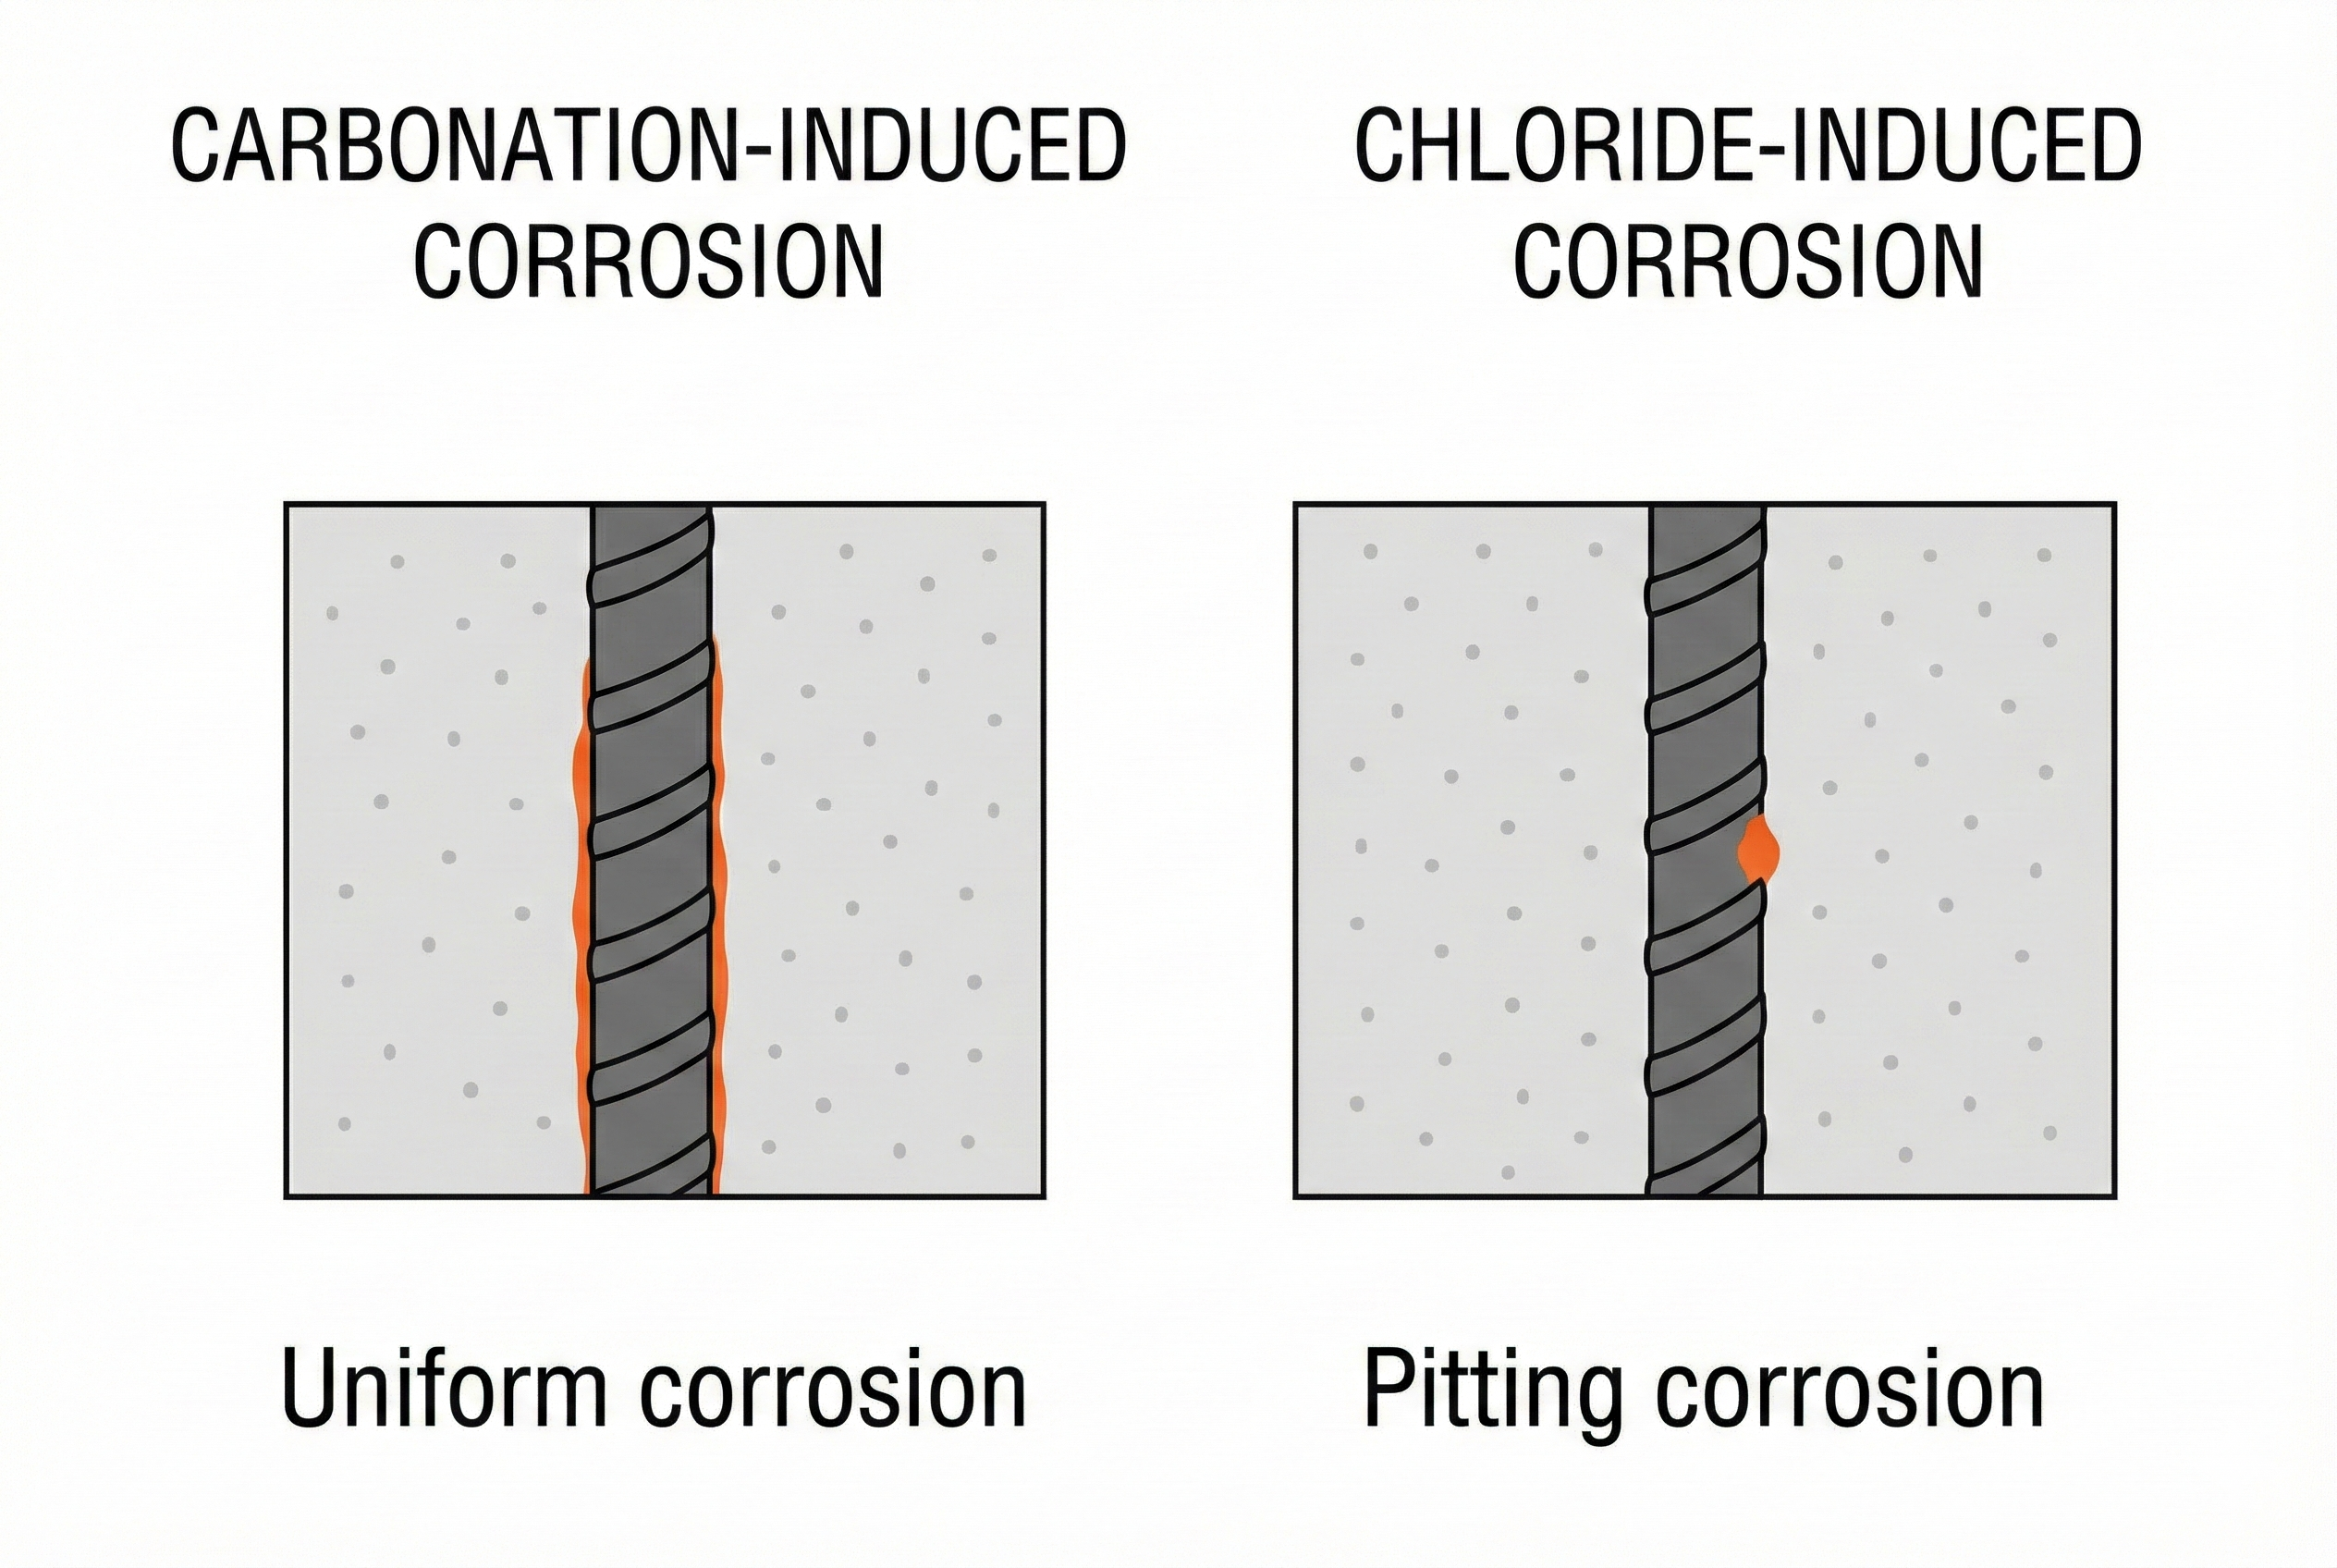
\includegraphics[width=0.5\linewidth]{z_corrosion_en.png}
    \caption{Corrosion differences.}
    \label{fig:z_corrosion_en}
\end{figure}

\subsection{Carbonation-induced corrosion phenomena}
Corrosion of steel reinforcement induced by carbonation represents one of the primary degradation mechanisms in reinforced concrete structures. The process initiates with the diffusion of atmospheric carbon dioxide (CO$_2$) through the concrete pore network. The CO$_2$ subsequently reacts with pore moisture and cement hydration products, predominantly calcium hydroxide (Ca(OH)$_2$), leading to the formation of calcium carbonate (CaCO$_3$).

This chemical reaction induces a substantial reduction in the concrete pore solution pH. Under normal conditions, concrete maintains a highly alkaline environment (pH range: 12.6--13.5), which sustains a stable passive oxide layer on the steel reinforcement surface, providing effective corrosion protection. However, the progressive advancement of the carbonation front reduces the pH to values below 9. This acidification of the concrete matrix initiates the depassivation of the reinforcement, rendering the steel susceptible to generalized corrosion in the presence of sufficient oxygen and moisture.

The speed and depth of carbonation are influenced by various environmental and material factors, such as: CO$_2$ concentration (higher levels accelerate the reaction); Relative Humidity (RH) (carbonation is most intense in intermediate ranges, typically 50\%--70\%); Concrete Quality (water/cement ratio, cement type, and porosity determine CO$_2$ ingress ease); and Cover thickness (acting as a physical barrier).

\subsection{Dataset}

This study employs a comprehensive dataset of carbonation progression in concrete structures, comprising 20,000 samples obtained from \citet{couto_machine_2025}. The dataset incorporates both numerical and categorical variables characterizing environmental conditions, material properties, and temporal factors influencing carbonation depth.

The dataset incorporates seven variables: two categorical and five numerical. The numerical input features encompass atmospheric CO$_2$ concentration (\%), 28-day concrete compressive strength $f_c$ (MPa), environmental relative humidity RH (\%), and exposure duration $t$ (years), while the target variable is the carbonation depth $y$ (mm).

Categorical variables include cement type and exposure conditions. The cement classification adheres to the Brazilian standard ABNT NBR 16697, where the acronym 'CP' denotes Portland Cement, followed by suffixes indicating the predominant supplementary cementitious material: 'E' for blast furnace slag, 'Z' for pozzolan, 'F' for carbonaceous filler, and 'ARI' for High Early Strength. Based on this standardization, the study analyzed six distinct types with varying clinker and supplementary material contents: CP V-ARI (>90\% clinker); CP II-E (70--80\% clinker, 15--25\% slag); CP II-F (70--80\% clinker, 10--20\% limestone); CP II-Z (70--80\% clinker, 15--25\% pozzolan); CP III (25--35\% clinker, 60--70\% slag); and CP IV (55--65\% clinker, 25--40\% pozzolan). Furthermore, environmental exposure conditions are classified as Protected Indoor (PIA), Protected Outdoor (PEA), or Unprotected Outdoor (UEA).

Table~\ref{tab:statistics} presents the basic descriptive statistics for the numerical variables. Figure~\ref{fig:histograms} complements this analysis by showing the distribution of each variable through individual KDE (Kernel Density Estimation), offering visual assessment of data spread and central tendencies. Carbonation depth in millimeters serves as the target variable for subsequent predictive modeling.

\begin{table}[htpb!]
    \centering
    \small
    \caption{Descriptive statistics of numerical variables in the carbonation dataset ($n = 20,000$).}
    \label{tab:statistics}
     \begin{tabular}{lrrrr}
    \toprule
     & \textbf{mean} & \textbf{std} & \textbf{min} & \textbf{max} \\
    \midrule
   \textbf{ CO2 (\%)} & 0.16 & 0.08 & 0.03 & 0.30 \\
   \textbf{ $f_c$ (MPa)} & 34.90 & 8.66 & 20.00 & 50.00 \\
    \textbf{RH (\%)} & 59.94 & 17.31 & 30.00 & 90.00 \\
    \textbf{Type of cement} & 2.51 & 1.71 & 0.00 & 5.00 \\
    \textbf{Exposure conditions} & 0.99 & 0.82 & 0.00 & 2.00 \\
    \textbf{$t$ (years)} & 49.93 & 29.32 & 0.00 & 100.00 \\
    \textbf{carb. depth (mm)} & 16.59 & 12.84 & 0.00 & 119.71 \\
    \bottomrule
    \end{tabular}
\end{table}

\begin{figure}[htpb!]
    \centering
    \begin{subfigure}[b]{0.35\textwidth}
        \centering
        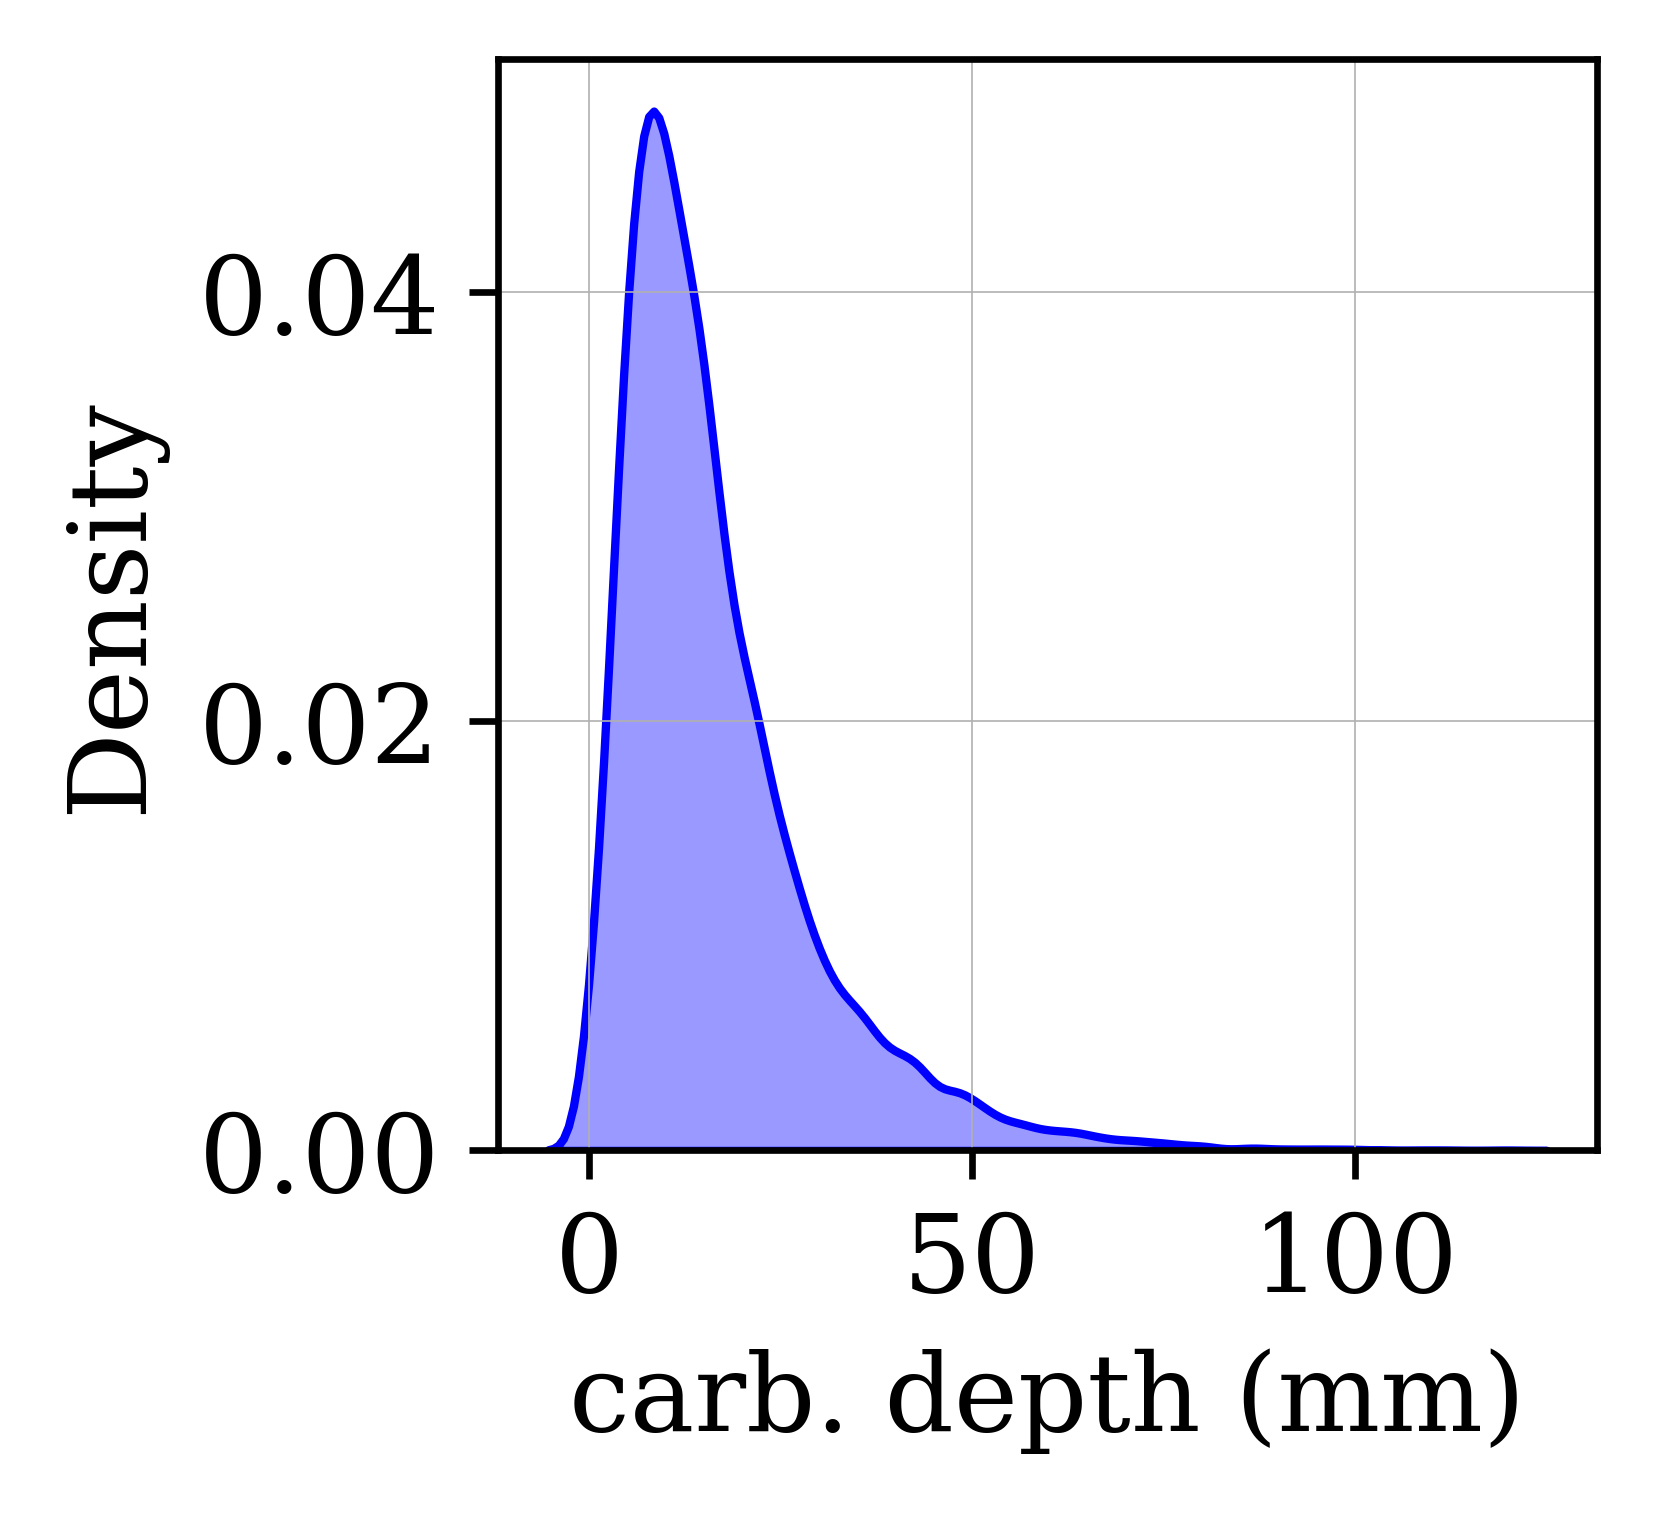
\includegraphics[width=1\linewidth]{z_kde_carbonation_depth.png}
        \caption{CO$_2$ concentration}
        \label{fig:hist_co2}
    \end{subfigure}
    \hfill
    \begin{subfigure}[b]{0.35\textwidth}
        \centering
        
\includegraphics[width=1\linewidth]{z_kde_compressive_strength.png}
        \caption{Concrete strength $f_c$}
        \label{fig:hist_fc}
    \end{subfigure}

    \vspace{0.3cm}

    \begin{subfigure}[b]{0.35\textwidth}
        \centering
        
\includegraphics[width=1\linewidth]{z_kde_relative_humidity.png}
        \caption{Relative humidity RH}
        \label{fig:hist_rh}
    \end{subfigure}
    \hfill
    \begin{subfigure}[b]{0.35\textwidth}
        \centering
        
\includegraphics[width=1\linewidth]{z_kde_time.png}
        \caption{Exposure time $t$}
        \label{fig:hist_time}
   \end{subfigure}

    \vspace{0.3cm}

    \begin{subfigure}[b]{0.35\textwidth}
        \centering
        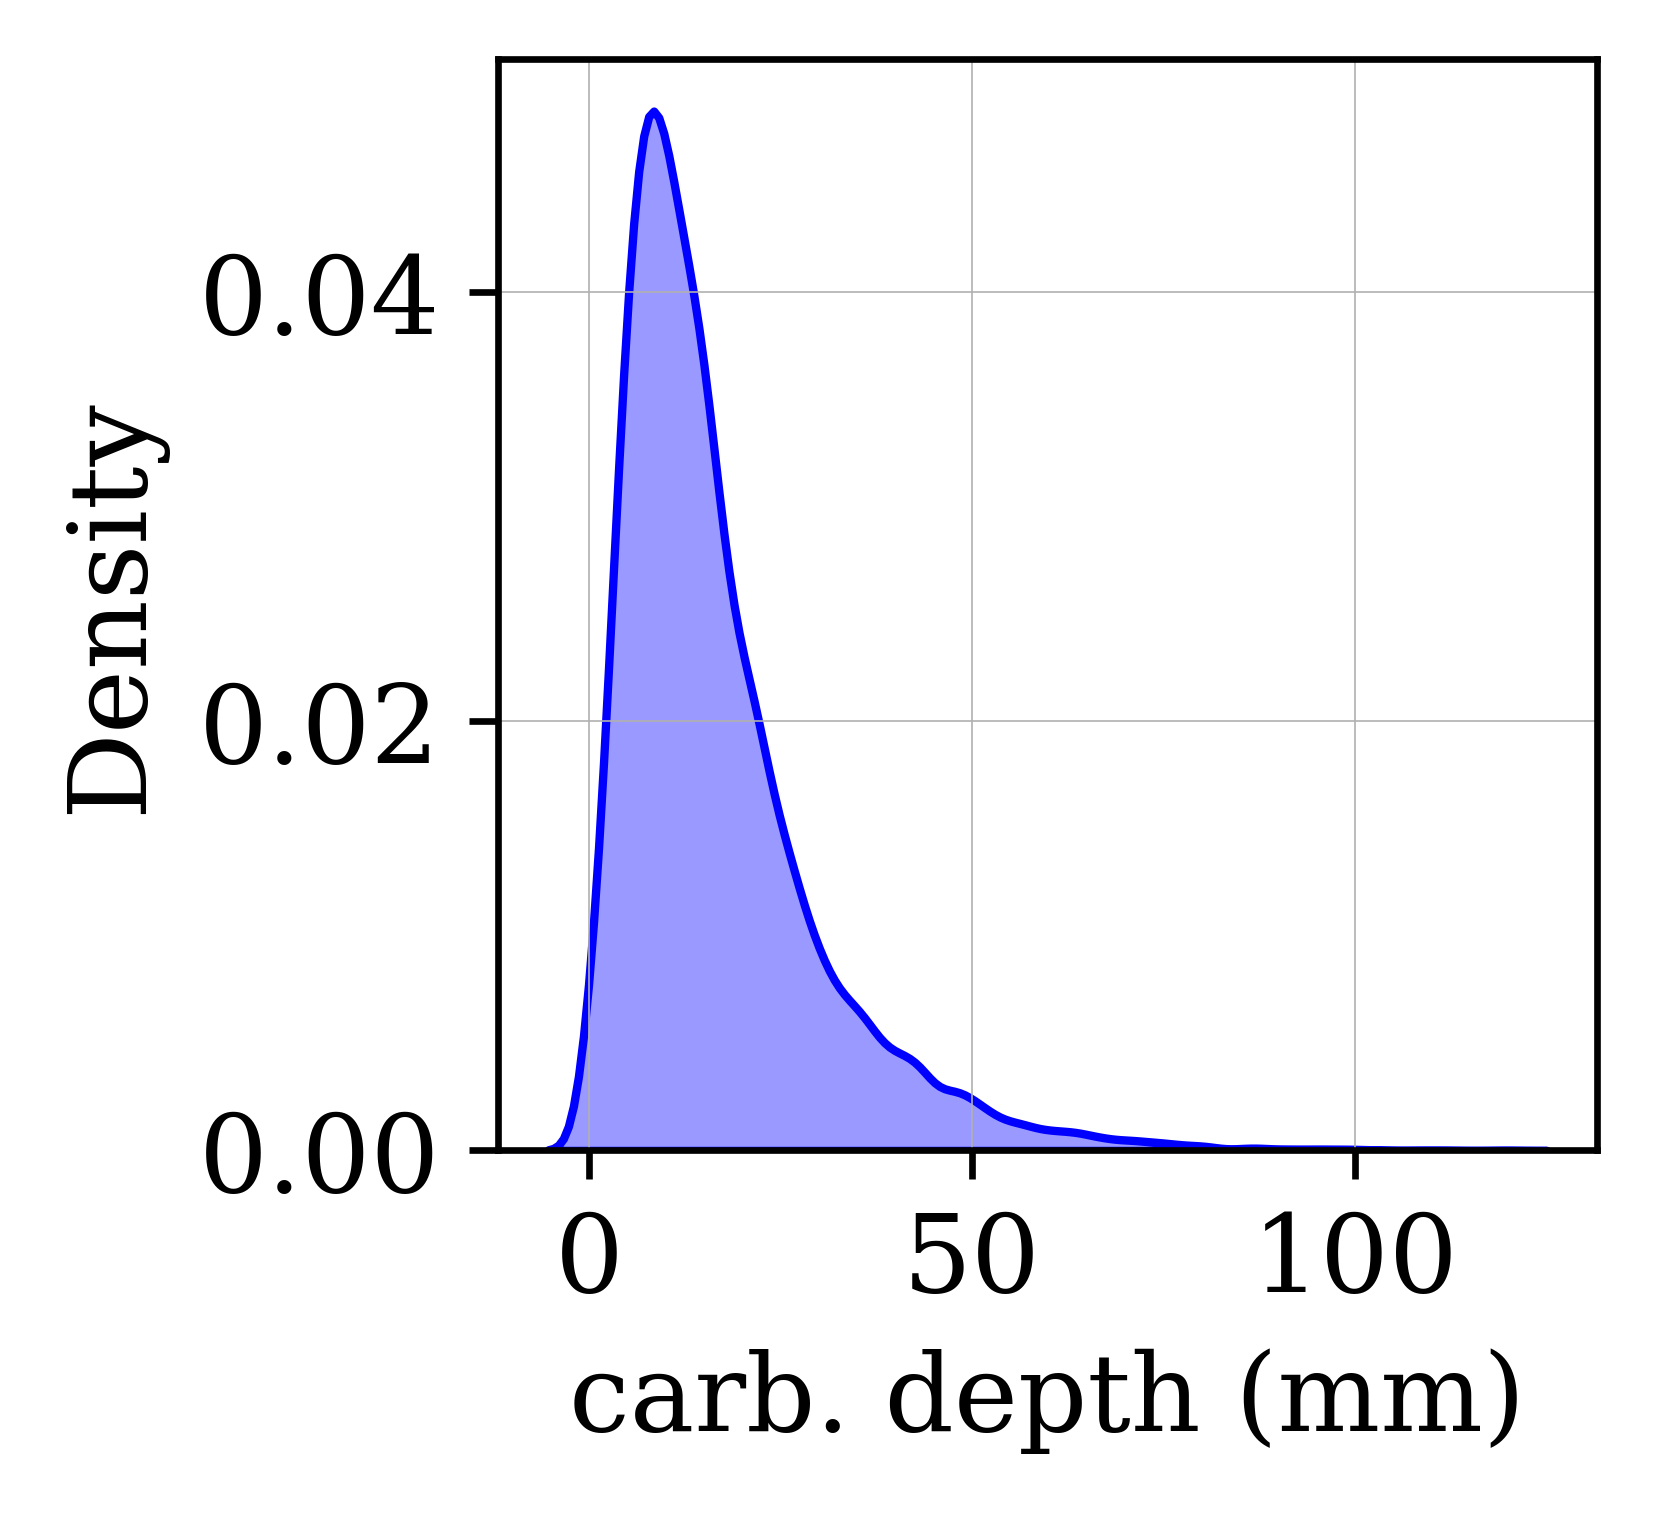
\includegraphics[width=1\linewidth]{z_kde_carbonation_depth.png}
        \caption{Carbonation depth $y$}
        \label{fig:hist_depth}
    \end{subfigure}

    \caption{Kernel Density Estimation (KDE) of numerical variables in the carbonation dataset.}
    \label{fig:histograms}
\end{figure}

The KDE plots reveal the statistical profile of the dataset. The concrete compressive strength ($f_c$) exhibits a multimodal distribution concentrated around commercial classes (20, 30 and 40 MPa). The environmental variables cover a representative range of exposure conditions, while the time variable ($t$) indicates that the dataset includes both young concrete and mature structures, providing a solid temporal basis for regression.

\subsection{Machine Learning approach}

\subsubsection{Training and test}
This study employs supervised machine learning, where algorithms learn a mapping function $f: X \to Y$ from labeled data to minimize prediction error on unseen samples. Among the regression models applied, the Multi-Layer Perceptron (MLP) stands out for its ability to approximate complex non-linear functions. Structurally, an MLP consists of input, hidden, and output layers composed of neurons. Each neuron computes a weighted sum of inputs plus a bias, which is then passed through a non-linear activation function. The network "learns" by iteratively adjusting these weights and biases using the backpropagation algorithm and an optimizer to minimize a specific loss function.

Based on this theoretical framework, the specific model in this work was implemented by feeding the input features directly into the network. The topology was configured with two hidden layers containing 100 and 50 neurons, respectively. The Rectified Linear Unit (ReLU) was employed as the non-linear activation function, while the Adaptive Moment Estimation (Adam) algorithm was selected as the solver for weight optimization.

Seven machine learning models were trained to predict carbonation depth in concrete structures. To ensure statistical robustness and mitigate overfitting, a 10-fold cross-validation strategy was employed. In each iteration, the dataset was randomly split into training (80\%) and testing (20\%) sets. Table~\ref{tab:model_performance} presents the mean $R^2$ scores evaluated on these independent test sets. Figure~\ref{fig:model_comparison} illustrates the comparison between predicted and observed values, with figure (a) showing the worst-performing model and figure (b) displaying the best-performing model.

\begin{table}[H]
    \centering
    \small
    \caption{Performance metrics ($R^2$) of machine learning models on the independent test set (20\% kfold). Values presented as Mean.}
    \label{tab:model_performance}
    \begin{tabular}{lcc}
        \toprule
        \textbf{Model} & \textbf{$R^2$ Train} & \textbf{$R^2$ Test} \\
        \midrule
        Linear Regression & 0.54 & 0.54 \\
        Ridge Regressor & 0.54 & 0.54 \\
        Lasso Regressor & 0.53 & 0.53 \\
        Decision Tree & 1.00 & 0.92 \\
        Random Forest & 0.99 & 0.96 \\
        Gradient Boosting & 0.95 & 0.94 \\
        Hist Gradient Boosting & 0.99 & 0.99 \\
        \textbf{Neural Network MLP} & \textbf{0.99} & \textbf{0.99} \\
        \bottomrule
        \multicolumn{3}{l}{\footnotesize \textit{Note: Standard deviation was omitted due to negligible values (magnitude $\le 1\%$) across all iterations.}} \\
    \end{tabular}

    \vspace{0.2cm}
\end{table}

\begin{figure}[htpb!]
    \centering
    \begin{subfigure}[b]{0.40\textwidth}
        \centering
        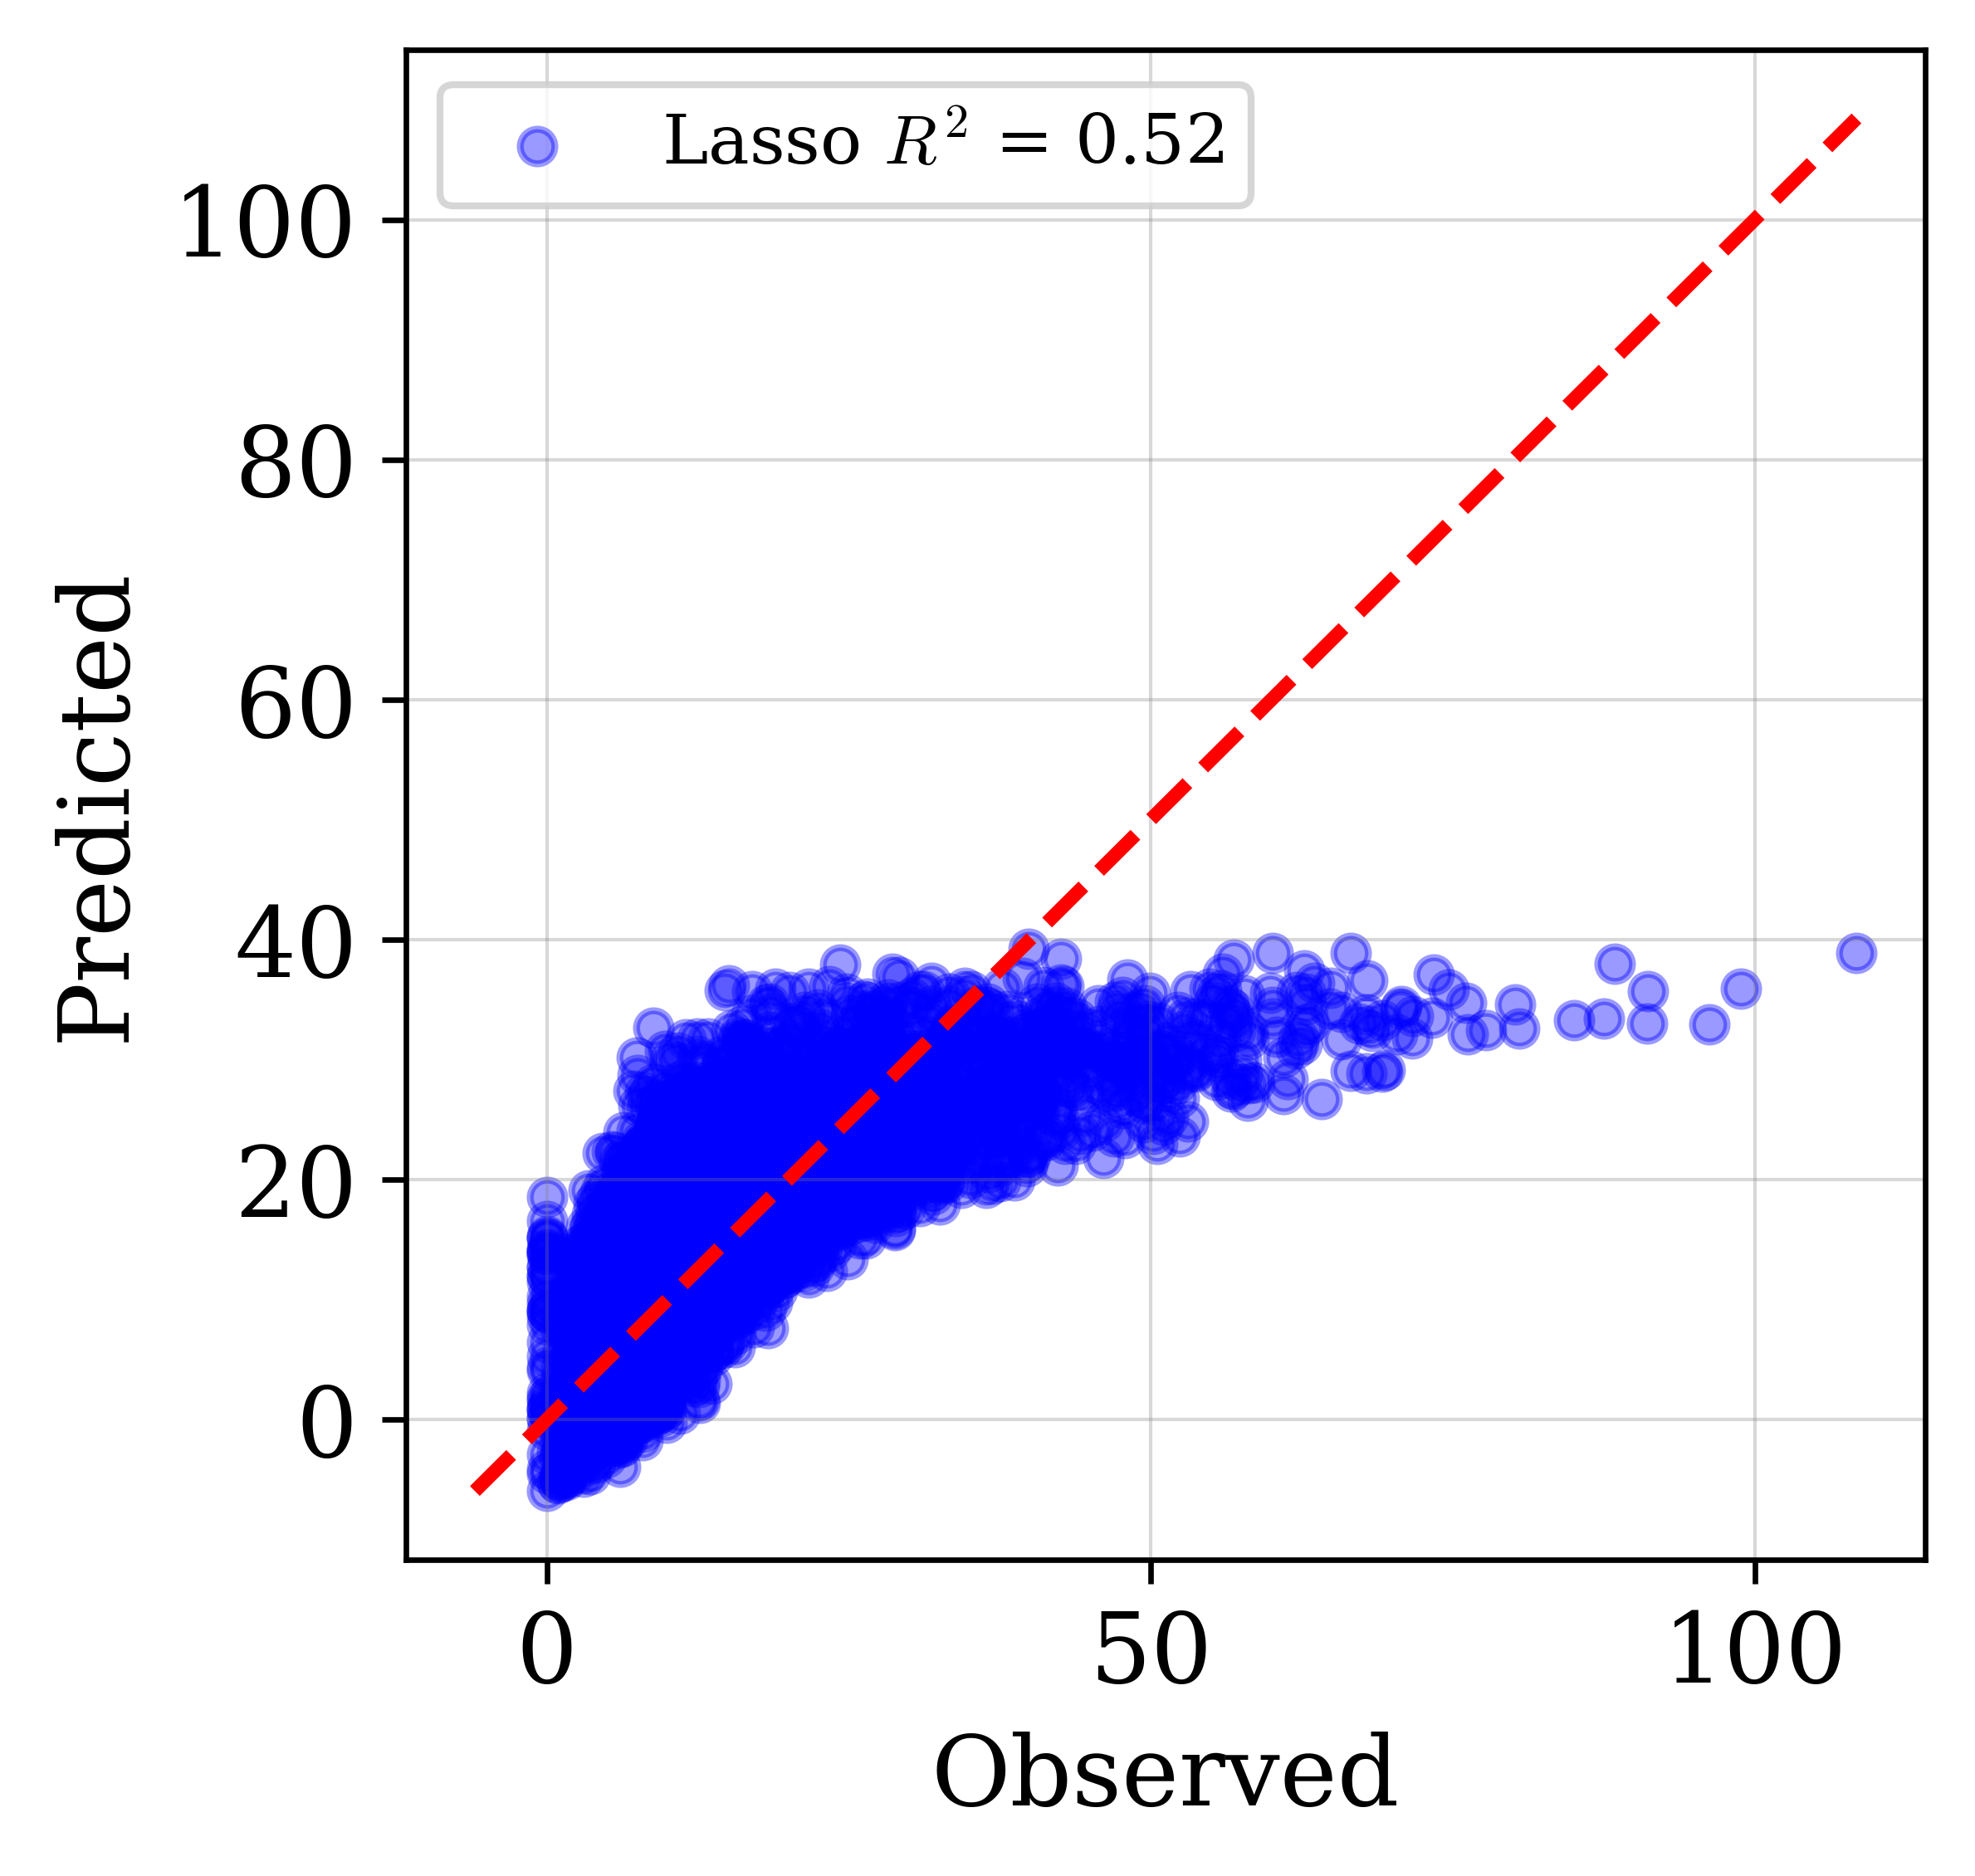
\includegraphics[width=\linewidth]{z_scatter_worst_model_en.png}
        \caption{Worst model: Lasso Regressor ($R^2 = 0.52$)}
        \label{fig:worst_model}
    \end{subfigure}
    \hfill
    \begin{subfigure}[b]{0.375\textwidth}
        \centering
        
\includegraphics[width=\linewidth]{z_scatter_best_model_en.png}
        \caption{Best model: Neural Network MLP ($R^2 = 0.99$)}
        \label{fig:best_model}
    \end{subfigure}
    \caption{Comparison between predicted and observed carbonation depth values for (a) the worst-performing and (b) best-performing models. The dashed line represents perfect prediction ($y=\hat{y}$).}
    \label{fig:model_comparison}
\end{figure}

The Figure \ref{fig:model_comparison} comparison between predicted and observed carbonation depth values for (a) the worst-performing model (Lasso, $R^2$ = 0.52) and (b) best-performing model (Neural Network MLP, $R^2$ = 0.99). The dashed line represents perfect prediction.

\subsubsection{CO2 profile}
To model the temporal evolution of atmospheric carbon dioxide ($CO_2$) concentration, a fundamental parameter for structural degradation simulations, an approach based on historical and instrumental records was adopted. For the initial historical period (1900 to 1950), the dataset derives from high-resolution paleoclimatic records extracted from Antarctic ice cores (Law Dome), which provide critical data covering the pre-industrial period to the 20th century and are managed by the NOAA National Centers for Environmental Information (NOAA/NCEI) \cite{noaa_law_dome}. From 1950 onwards, the model is anchored in continuous direct atmospheric measurements provided by the NOAA Global Monitoring Laboratory (GML) at the Mauna Loa observatory in Hawaii \cite{noaa_gml}, alongside records from the World Data Centre for Greenhouse Gases (WDCGG) \cite{wmo_wdcgg}.

For use in this research, a piecewise analytical regression was created to simulate this $CO_2$ accumulation profile, yielding a coefficient of determination ($R^2$) of 0.99. The mathematical framework divides the time series into three continuous regimes of anthropogenic growth, illustrated in Figure \ref{fig:evolution_co2}. These include a slow linear growth between 1900 and 1950, an accelerated linear growth between 1950 and 2000, and a quadratic growth post-2000, capturing the contemporary intensification of global emissions.

To illustrate the practical application of the described models, parametric simulations were conducted projecting the carbonation advancement for the extended period from 1900 to 2150. The subsequent graphs present the temporal evolution of the carbonation front, highlighting the direct influence of the concrete compressive strength class ($f_{ck}$) (Figure \ref{fig:evolution_fck}) and the environmental relative humidity (Figure \ref{fig:evolution_h}) on the degradation rate. For service life assessment purposes, a reference line was set at 30 mm, corresponding to a typical normative concrete cover \cite{nbr6118}, indicating the theoretical threshold for reinforcement depassivation.

\begin{figure}
    \centering
    
\includegraphics[width=0.5\linewidth]{z_graph_1900_co2.png}
    \caption{Evolution of Carbonation by $CO_2$}
    \label{fig:evolution_co2}
\end{figure}

Figure \ref{fig:evolution_co2} piecewise regression curve of atmospheric carbon dioxide ($CO_2$) concentration simulated from 1900 to 2150. The graph illustrates the model's transitions between the slow linear historical regime (pre-1950), the accelerated linear regime (1950–2000), and the contemporary quadratic non-linear behavior (post-2000) projecting future accumulations.

\begin{figure}
    \centering
    
\includegraphics[width=0.5\linewidth]{z_graph_1900_fck.png}
    \caption{Evolution of Carbonation by $fck$}
    \label{fig:evolution_fck}
\end{figure}

Figure \ref{fig:evolution_fck} temporal evolution of carbonation depth for different compressive strength classes ($f_{ck}$), considering a constant relative humidity of 65\% (critical scenario) and a normative concrete cover of 30 mm, simulated for the period from 1900 to 2150.

\begin{figure}
    \centering
    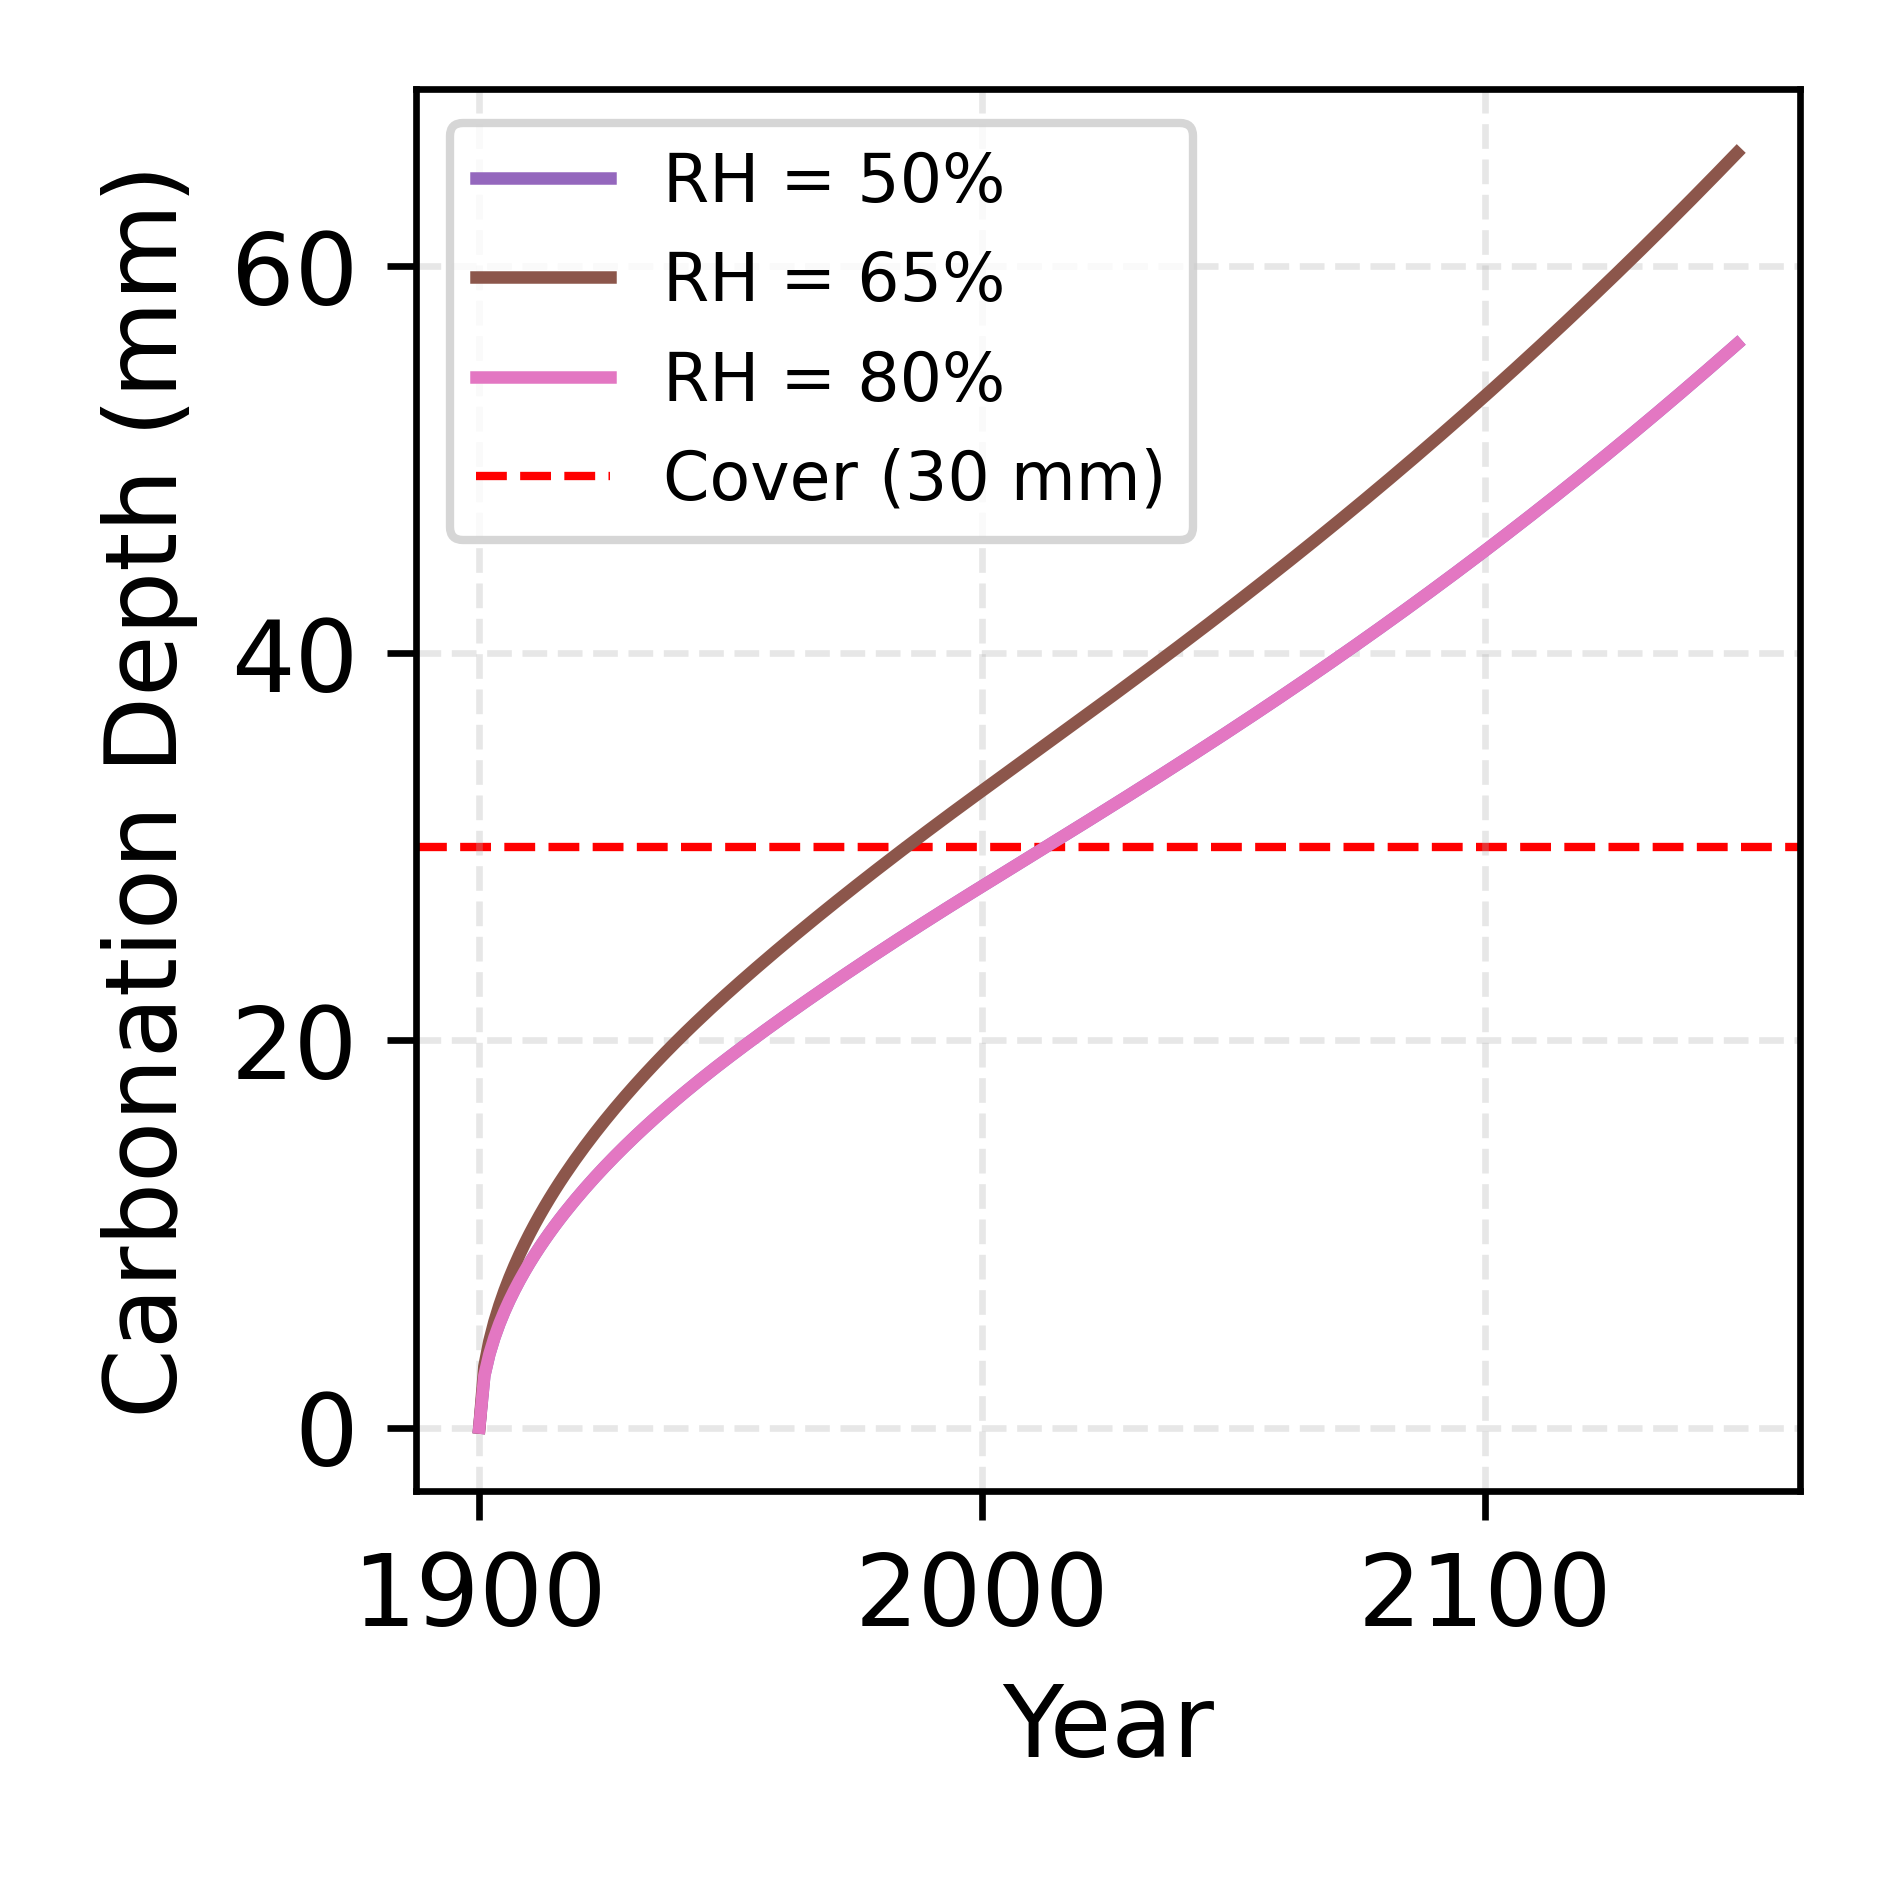
\includegraphics[width=0.5\linewidth]{z_graph_1900_h.png}
    \caption{Evolution of Carbonation by humidity}
    \label{fig:evolution_h}
\end{figure}

Figure \ref{fig:evolution_h} influence of relative humidity on the advancement of the carbonation front over time for concrete with an $f_{ck}$ of 30 MPa. The graph highlights the acceleration of degradation in environments with intermediate humidity (65\%) compared to drier (50\%) or more humid (80\%) environments, simulated for the period from 1900 to 2150.

\subsubsection{Carbonation profile}

Carbonation depth profiles were analyzed to determine the carbonation coefficient ($k$), a key parameter characterizing the rate of carbonation progression. The coefficient $k$ is obtained by rearranging the carbonation depth law (Equation as $k = y / \sqrt{t}$, where $y$ represents carbonation depth (mm) and $t$ denotes exposure time (years).
Figure \ref{fig:z_carbonation_profile} presents the average carbonation coefficient along with four representative carbonation depth profiles. The figure illustrates profiles for indoor exposure conditions (AIP), which exhibited the highest carbonation rates across all strength classes. 

\begin{figure}[htpb!]
        \centering
        
\includegraphics[width= 0.60\textwidth]{z_carbonation_profile.png}
        \caption{Indoor exposure (AIP) profiles. Carbonation coefficients: k20 = 5.8, k30 = 3.8, k40 = 2.3, k50 = 1.7 mm/sqrt(year)}
        \label{fig:z_carbonation_profile}
    \end{figure}

    
\subsection{Machine Learning}

Machine Learning (ML) is a subfield of Artificial Intelligence focused on the development of algorithms capable of learning patterns and making inferences from data without being explicitly programmed for specific rules. Unlike the traditional deterministic approach, where an expert defines the physical equations governing the phenomenon, ML models induce mathematical relationships directly from empirical observations.

This paradigm relies on generalization capability: the algorithm analyzes a training dataset to construct a model capable of making accurate predictions on new, unseen data. ML techniques are broadly categorized into supervised, unsupervised, and reinforcement learning. In the context of predicting the service life of structures, supervised learning is predominant. Here, the model is trained with known input-output pairs, enabling the mapping of complex, non-linear interactions that often elude conventional analytical formulations.

\subsection{Neural Networks}

Artificial Neural Networks (ANNs) are computational models inspired by the biological neural networks of the human brain. As a fundamental subset of machine learning and deep learning, ANNs are designed to recognize complex patterns, map non-linear relationships, and process large volumes of data. The architecture of a standard neural network is structured into three main parts: an input layer, one or more hidden layers, and an output layer. These layers are composed of interconnected nodes, known as artificial neurons, which process information by applying synaptic weights and activation functions. During the training phase, the network employs optimization algorithms, such as backpropagation, to iteratively adjust these mathematical weights in order to minimize the loss function (error). This continuous adjustment process grants the model the ability to autonomously learn and generalize solutions from the provided data.

\subsection{Theoretical Background: Histogram-based Gradient Boosting Regressor (HGBR)}

The \textit{Histogram-based Gradient Boosting Regressor} (HGBR) is an advanced machine learning technique belonging to the \textit{Gradient Boosting Decision Trees} (GBDT) family. This approach is grounded in the principle of ensemble learning, where multiple simple predictive models—termed "weak learners"—are combined sequentially to form a robust and high-precision predictor.

\subsubsection{Boosting Mechanism}

The core operation of the algorithm is based on the additive construction of decision trees. Unlike models such as \textit{Random Forest}, which build independent trees in parallel, HGBR constructs trees sequentially. Each new tree is trained specifically to correct the residual errors (the difference between the actual and predicted values) made by the ensemble of previous trees.

Mathematically, the final prediction $\hat{y}_i$ for a given input $x_i$ is the sum of the predictions of $K$ trees:

\begin{equation}
    \hat{y}_i = \sum_{k=1}^{K} f_k(x_i), \quad f_k \in \mathcal{F}
\end{equation}

Where $\mathcal{F}$ represents the function space of all possible regression trees. The optimization process seeks to minimize an objective function at each iteration $t$, composed of a differentiable loss function $l$ (such as Mean Squared Error) and a regularization term $\Omega$:

\begin{equation}
    \mathcal{Obj}^{(t)} = \sum_{i=1}^{n} l(y_i, \hat{y}_i^{(t-1)} + f_t(x_i)) + \Omega(f_t)
\end{equation}

\subsubsection{Histogram Strategy}

The main innovation of HGBR lies in its computational efficiency. Traditional \textit{Gradient Boosting} algorithms require sorting all values of each continuous feature to find the ideal split point at every tree node, resulting in a high computational cost of $\mathcal{O}(n \log n)$, where $n$ is the number of samples.

HGBR overcomes this limitation through the \textbf{discretization of data into histograms} (hence the name \textit{Histogram-based}). The algorithm groups continuous input variable values into discrete integer bins, typically limited to 256 values (8 bits). 

The process proceeds through a sequence of optimized stages. Initially, via \textbf{Binning (Mapping)}, continuous variables are mapped to discrete integers $b \in \{0, \dots, B-1\}$, where $B$ is the maximum number of bins, drastically reducing the cardinality of the analyzed data. Subsequently, during \textbf{Histogram Construction}, for each tree node, the algorithm constructs a histogram that accumulates the gradients ($g$) and hessians ($h$)—the first and second derivatives of the loss function—for each bin, an operation with linear complexity $\mathcal{O}(n)$. Following this, in the \textbf{Split Finding} phase, instead of iterating over all individual samples, the tree seeks the best split point by iterating only over the histogram bins, reducing the complexity to $\mathcal{O}(B)$, where $B \ll n$. Finally, to further accelerate training, the algorithm utilizes \textbf{Histogram Subtraction}, where the histogram of a child node is calculated by simply subtracting the sibling node's histogram from the parent node's histogram ($Hist_{child} = Hist_{parent} - Hist_{sibling}$), thereby eliminating the need to rescan the data.

\subsubsection{Handling of Missing Values}

An intrinsic feature of this architecture is its native support for missing values. During training, samples with missing data do not need to be imputed. The algorithm automatically learns, for each decision point, whether these samples should be directed to the left or right branch of the tree, based on which direction maximizes the reduction of the loss function (information gain).

This combination of sequential boosting, efficient discretization, and robust data handling makes HGBR capable of modeling complex non-linearities with high training speed and low memory consumption.

\subsection{Performance Evaluation Metrics}

The effectiveness of the proposed regression models was quantified using two complementary statistical metrics: the Coefficient of Determination ($R^2$) and the Adjusted Coefficient of Determination ($R^2_{adj}$). The use of these metrics allows for assessing the model's explanatory capacity weighted by its complexity.

The Coefficient of Determination ($R^2$) indicates the proportion of variance in the dependent variable (carbonation depth) that is predictable from the independent variables. Values range from 0 to 1, where values close to 1 indicate that the model captured most of the patterns present in the data, as shown in Equation \ref{eq:r2}:

\begin{equation}
    R^2 = 1 - \frac{\sum_{i=1}^{n} (y_i - \hat{y}_i)^2}{\sum_{i=1}^{n} (y_i - \bar{y})^2}
    \label{eq:r2}
\end{equation}

Where $y_i$ is the observed value, $\hat{y}_i$ is the predicted value, and $\bar{y}$ is the mean of the observed values.

However, the traditional $R^2$ tends to increase mechanically with the addition of new variables to the model, even if they lack statistical relevance. To mitigate this bias, the Adjusted $R^2$ ($R^2_{adj}$) is used, which incorporates a penalty based on the number of predictors. This metric offers a fairer assessment of the model's generalization and is calculated according to Equation \ref{eq:r2_adj}:

\begin{equation}
    R^2_{adj} = 1 - (1 - R^2) \frac{n - 1}{n - p - 1}
    \label{eq:r2_adj}
\end{equation}

Where $n$ represents the total number of samples and $p$ is the number of independent variables (features) in the model. Thus, an increase in the $R^2_{adj}$ value confirms that the complexity added to the model resulted in a real gain in predictive capacity.

\subsubsection{Relative Entropy or Kullback–Leibler divergence}

Considere uma variável aleatória discreta $X$   com função massa de probabilidade
\[
p(x)=P(X=x), \qquad x \in X.
\]

A entropia relativa ou distância de Kullback--Leibler entre duas
funções de massa de probabilidade $p(x)$ e $q(x)$ é definida por \cite{cover2006elements}
\begin{equation}
D(p\|q)
=
\sum_{x \in \mathcal{X}} p(x)
\log \frac{p(x)}{q(x)}
\label{eq:kl_discreta}
\end{equation}


Na definição acima, utilizamos a convenção de que
$$
0 \log \frac{0}{0} = 0, \ \ \ \ 0 \log \frac{0}{q} = 0 \ \  \text{e} \ \ \ p \log \frac{p}{0} = \infty.
$$
 
 
Assim, se existir algum símbolo $x \in  X $ tal que
$p(x) > 0$ e $q(x)=0$, então
\[
D(p\|q)=\infty.
\]
%%%%%%%%%%%%%%%%%%%%%% 
  Para o caso contínuo, a entropia
relativa ou divergência de Kullback--Leibler entre duas funções densidades de
probabilidade $p(x)$ e $q(x)$ é definida por
\begin{equation}
D(p\|q)
=
\int p(x)\log\frac{p(x)}{q(x)}\,dx.
\label{eq:kl_continua}
\end{equation}

%%%%%%%%%%%%%%%%%%%%%%%%%%%%%%%%%
A entropia relativa é sempre não negativa e é igual a zero se, e somente se,
$p=q$. ela  não é simétrica e não satisfaz a desigualdade triangular. Ainda assim,
é frequentemente útil interpretar a entropia relativa como uma medida de
``distância'' entre distribuições \cite{cover2006elements}.


\section{Evaluate of flexural strength}\label{sec:concrete}Nesta seção serão apresentados os modelos para previsão da resistência resudial de vigas de concreto armado sujeitas a carga distribuída. Este trabalho tomou como base a o trablho de Murilo [x]. Portanto esta seção será dividida em duas partes a primeira parte trata da resistência de vigas de concreto sem efeito da corrosão. A seção subsequente trata do modelo para previsão da resistência residual conforme descrito em Murilo[x] and Al-Ghoi [x].

O efeito corosão por carbonatação

As seções subsequentes tratam destas avaliações


\subsection{Computing Residual Flexure Strength}

O problema de concreto será tomado como a resitência a flexão pura conforme a maioria dos codigos de projeto tratam. Para isso toma-se a equação de equilibrio para forças normais para peças com armadura simples, dada pela equação tal.

xxxxxxxxxx

Para solução deste equação pretende-se dteemrinar qual o valor da ratio beta. Essa proposta é resolvida através do método da bi-seção e então determina-se o valor da posiçãop linha neutra e consequentemente o valor do momento resistente conforme equação tal.

\subsection{Computing Residual Flexure Strength with corrosion}

Primeiro explica o efeito da corosão na área de aço. Quanto reduz?

Explica a correção do MRd*.



Lorem Ipsum is simply dummy text of the printing and typesetting industry. Lorem Ipsum has been the industry's standard dummy text ever since the 1500s, when an unknown printer took a galley of type and scrambled it to make a type specimen book. It has survived not only five centuries, but also the leap into electronic typesetting, remaining essentially unchanged. It was popularised in the 1960s with the release of Letraset sheets containing Lorem Ipsum passages, and more recently with desktop publishing software like Aldus PageMaker including versions of Lorem Ipsum.

\subsection{Carbonation-induced corrosion phenomena}

\subsection{Carbonation-induced corrosion phenomena}

\subsection{Computing Residual Flexure Strength}

The model proposed by \cite{possan2010} offers a parametric approach to predict the carbonation depth ($y(t)$) in reinforced concrete structures, integrating material and environmental variables. The mathematical formulation, expressed in Equation \eqref{eq:y}, estimates the advance of the carbonation front over time, considering the influence of compressive strength ($f_c$), cement type, mineral admixtures, $CO_2$ concentration, and relative humidity ($RH$).

\begin{equation}\label{eq:y}
y(t) = k_c \cdot \left( \frac{20}{f_c} \right)^{k_{fc}} \cdot \left( \frac{t}{20} \right)^{\frac{1}{2}} \cdot \exp \left[ \frac{k_{ad} \cdot ad^{\frac{3}{2}}}{40 + f_c} + \frac{k_{CO_2} \cdot CO_2^{\frac{1}{2}}}{60 + f_c} - \frac{k_{RH} \cdot (RH - 0.58^2)}{100 + f_c} \right] \cdot k_{ce}
\end{equation}

Corrosion subsequent to carbonation is treated as an electrochemical phenomenon dependent on the presence of an electrolyte (pore water) and oxygen. The pH reduction induced by carbonation depassivates the reinforcement, allowing the formation of galvanic cells. Consequently, the corrosion rate is governed by the concrete's electrical resistivity and moisture availability. These factors are typically mitigated in design codes (e.g., ABNT NBR 6118) through the control of the water/cement ratio and cover thickness based on the environmental aggressiveness class.

\subsubsection{Calculation of Concrete Beams without Carbonation Corrosion}

The calculation of reinforced concrete beams without carbonation-induced corrosion ($t=0$) follows the guidelines of NBR 6118 \cite{associacao_brasileira_de_normas_tecnicas_nbr_2023}. The resisting bending moment ($M_{Rd}$) is determined by the equilibrium of forces in the cross-section, considering the non-linear behavior of the materials and the simplified rectangular stress block for the compressed concrete.

The design compressive strength of concrete, $f_{cd}$, and the design yield strength of steel, $f_{yd}$, are obtained by applying the respective partial safety factors ($\gamma_c$ and $\gamma_s$). The geometric parameters of the stress block ($\lambda_c$, $\alpha_c$, and $\eta_c$) are defined as a function of the characteristic strength $f_{ck}$, adjusting the stress distribution according to the concrete class, as expressed in the standard equations.

The neutral axis depth ($x$) is the governing variable of the problem and is determined through the equilibrium between the normal compressive force in the concrete and the tensile force in the reinforcement. Due to physical and geometric non-linearities, the solution for $x$ is obtained via an iterative numerical bisection method, which seeks the root of the equilibrium function $f_\alpha(\beta) = 0$ within a predefined interval. Once the value of $x$ converges, the resisting moment is calculated by Equation \eqref{eq:mrd_lim_resumida}:

\begin{equation}\label{eq:mrd_lim_resumida}
M_{Rd} = \sigma_{cd} \cdot (\lambda_c \cdot x \cdot b_w) \cdot (d - 0.5 \cdot \lambda_c \cdot x)
\end{equation}

Where $b_w$ is the section width, $d$ is the effective depth, and the term in parentheses represents the internal lever arm. This value establishes the performance baseline of the structure before the onset of degradation due to corrosion.

\subsection{Action of $CO_2$ on Concrete Structures}

In the context of the durability of concrete structures, atmospheric carbon dioxide ($CO_2$) acts as one of the main aggressive agents, and its interaction with the cementitious matrix triggers the carbonation process.

The $CO_2$ present in the air diffuses through the pore and capillary network of the concrete cover. In the presence of moisture, the gas reacts chemically with the hydrated compounds of the cement paste, primarily calcium hydroxide, converting it into calcium carbonate and water.

The structurally critical effect of $CO_2$ is consolidated when the carbonation front advances in depth and reaches the reinforcement level. The subsequent drop in pH thermodynamically destabilizes the passivating film, which is destroyed, leaving the steel unprotected. This phenomenon is known as depassivation.

From this point on, the corrosion propagation phase begins, which tends to be generalized and uniform along the affected steel bar. This process generates corrosion products (iron oxides and hydroxides) whose specific volume is significantly greater (often three to six times) than that of the original consumed steel. This volumetric expansion generates internal tensile stresses in the concrete that exceed the tensile strength of the material, causing cracking and cover spalling.

Finally, the ongoing action of $CO_2$ results in a continuous loss of the reinforcement's effective cross-sectional area and the degradation of the bond between steel and concrete, severely compromising the load-bearing capacity of the structure.

\subsubsection{Carbonation-Induced Corrosion}

In reinforced concrete structures, the concrete cover acts as a physical barrier and provides chemical protection through the high alkalinity of the pore solution, which maintains a passive oxide layer on the steel surface. The corrosion process is typically divided into two phases: initiation, where the reinforcement remains passive, and propagation, where the protective layer is destroyed, and active corrosion begins \cite{cavaco_reliabilitybased_2017}.

Unlike chloride-induced corrosion, which causes localized pitting, carbonation results in generalized corrosion distributed along the reinforcement. Atmospheric carbon dioxide ($CO_2$) diffuses into the concrete pores and reacts with calcium hydroxide ($Ca(OH)_2$), reducing the pH from its original values (12.5--13.5) to levels below 9. This reaction is described by Equation \eqref{eq:carbonation}:

\begin{equation}\label{eq:carbonation}
\mathrm{Ca(OH)_2 + CO_2 \rightarrow CaCO_3 + H_2O}
\end{equation}

The pH reduction leads to the depassivation of the steel. The subsequent formation of iron oxides, which have a larger volume than the original metal, generates internal expansive stresses. These stresses cause cracking and spalling of the concrete cover, accelerating the ingress of aggressive agents. Ultimately, structural safety is compromised by the reduction of the reinforcement cross-sectional area and the degradation of the steel-concrete bond \cite{tuutti_corrosion_1982, soltani_state---art_2019}.

\subsubsection{Residual Strength of Beams Subjected to Corrosion}

The analysis of the residual load-bearing capacity of reinforced concrete beams under corrosion effects considers multiple degradation stages, primarily the loss of reinforcement cross-sectional area and the deterioration of the bond between steel and concrete \cite{possan_co2_2016, Azad2010}. The calculation of the residual resisting moment ($M_{res}$) is performed in two steps: first, the strength of the section with corroded reinforcement ($M_{res,cor}$) is determined, and then a correction factor ($C_f$) is applied to account for bond loss, as shown in Equations \eqref{eq:m_res} and \eqref{eq:c_f}:

\begin{equation}\label{eq:m_res}
M_{res} = C_f \cdot \left[ A_{s,cor} \cdot f_y \cdot \left( d - \frac{\lambda}{2} x \right) \right]
\end{equation}

\begin{equation}\label{eq:c_f}
C_f = \frac{5.0}{d_{s0}^{0.54} \cdot (i_{cor,u} \cdot t_y)^{0.19}} \leq 1.0
\end{equation}

The reduced cross-sectional area ($A_{s,cor}$) is derived from the residual bar diameter ($d_{cor}$), which decreases linearly as a function of the corrosion rate ($i_{cor,u}$) and the exposure time after depassivation ($t_c$), according to the model by \textcite{pellizzer_time-dependent_2020}:

\begin{equation}\label{eq:d_cor}
d_{cor} = d_{s0} - 0.0232 \cdot i_{cor,u} \cdot t_c
\end{equation}

For a more accurate estimation, the corrosion rate ($i_{cor,u}$) is not considered constant. Instead, it is adjusted based on temperature variations ($T(t)$) and the environmental exposure class, as proposed by \textcite{peng_climate_2016}:

\begin{equation}\label{eq:i_cor_t}
i_{cor,u} = i_{cor,20} \cdot \left[ 1 + K \cdot (T(t) - 20) \right]
\end{equation}
\section{Results}\label{sec:res}\subsection{Toy problem}

To verify the proposed methodological pipeline, an adapted version of the toy problem introduced by \citet{pires_reliability_2024} is adopted in this section and defined by Equation \eqref{eq:toy_problem_equation}. In this formulation, \textbf{R} and \textbf{S} denote the structural resistance and the load demand, respectively. The limit-state function $g(\cdot)$ is defined to explicitly account for time-dependent degradation and modeling uncertainties within a probabilistic framework.

Time dependency is introduced through a linear degradation factor applied to the resistance variable, represented by the function $k_{\text{factor}}(t)$. This factor models a progressive reduction in resistance capacity over the service life, assuming $k_{\text{initial}} = 1.0$ at the initial time and $k_{\text{final}} = 0.3$ at the end of the considered lifetime, $T_f = 100$ years, as expressed in Equation \eqref{eq:k_factor_linear}. Although simplified, this formulation captures the essential effects of long-term deterioration processes commonly considered in structural reliability analyses.

Modeling uncertainties are incorporated through the latent variables $\textbf{Z}_1$ and $\textbf{Z}_2$, which affect the resistance and load terms, respectively. These latent variables are modeled as random variables, introducing additional variability into the realizations of \textbf{R} and \textbf{S} and allowing the uncertainty propagation to be explicitly represented in the limit-state function.

The complete formulation of the adopted limit-state function is presented in Equation \eqref{eq:toy_problem_equation}. The probabilistic characterization of all random variables involved in the model, including their probability distributions and statistical parameters, is summarized in Table~\ref{tab:random_variables_parameters}. Normal distributions are assumed for the resistance and load variables, while lognormal distributions are adopted for the model uncertainty factors, following standard practice in structural reliability modeling.

\begin{equation}
k_{\text{factor}}(t) = 
\begin{cases} 
k_{\text{initial}}, & t \leq 0 \\[5pt]
k_{\text{final}}, & t \geq T_f \\[5pt]
k_{\text{initial}} + (k_{\text{final}} - k_{\text{initial}}) \cdot \dfrac{t}{T_f}, & 0 < t < T_f 
\end{cases}
\label{eq:k_factor_linear}
\end{equation}

\begin{equation}
g(\textbf{R}, \textbf{S}, t) = k_{\text{factor}}(t) \cdot \frac{\textbf{R}}{\textbf{Z}_1} - \textbf{S} \cdot \textbf{Z}_2
\label{eq:toy_problem_equation}
\end{equation}

\begin{table}[H]
\centering
\caption{Statistical parameters and probability distributions of the variables used in the model}
\label{tab:random_variables_parameters}
\begin{tabular}{l c c c c}
\hline
\textbf{Variable} & \textbf{Symbol} & \textbf{Distribution} & \textbf{Mean} & \textbf{Standard Deviation} \\
\hline
Resistance      & $R$     & Normal      & 5.00 & 0.80  \\
Load realization            & $S$     & Normal      & 2.00 & 0.60  \\
Model uncertainty for resistance  & $Z_1$   & Lognormal  & 1.00 & 0.028 \\
Model uncertainty for load & $Z_2$   & Lognormal  & 1.00 & 0.096 \\
\hline
\end{tabular}
\end{table}

The time-dependent analysis is performed considering 10 equally spaced time steps over a 100-year horizon. At each time step, realizations of the limit-state function $g$ are evaluated, enabling the assessment of its temporal evolution. In parallel, the corresponding values of the four GLAM parameters, $\lambda_1$ to $\lambda_4$, are computed and analyzed.

For illustrative purposes, fixed realizations of the resistance and load variables, $r = 5.09$ and $s = 1.80$, are considered together with 2000 samples of the latent variables at each time step. The resulting dataset is depicted in Figure~\ref{fig:g_function_realizations}. Figure~\ref{fig:g_function_realizations}(a) shows the evolution of the limit-state function over time, clearly reflecting the influence of the degradation factor applied to the resistance. Figure~\ref{fig:g_function_realizations}(b) presents the temporal evolution of the GLAM parameters, highlighting distinct trends among $\lambda_1$--$\lambda_4$.
\begin{figure}[H]
    \centering

    \begin{subfigure}{0.9\textwidth}
        \centering
        
\includegraphics[width=\textwidth]{z_time-lapse_g_analysis_en.png}
        \caption{}
        \label{fig:indoor_profiles}
    \end{subfigure}

    \vspace{0.5cm} % espaço vertical entre as figuras

    \begin{subfigure}{0.95\textwidth}
        \centering
        
\includegraphics[width=\textwidth]{z_lambdas_for_r_s_realization_en.png}
        \caption{}
        \label{fig:outdoor_profiles}
    \end{subfigure}

    \caption{Evaluation of the function $g$ over time points. 
    (a) Realizations with fixed values $r = 5.09$ and $s = 1.80$. 
    (b) $\lambda_1$--$\lambda_4$ over the time.}
    \label{fig:g_function_realizations}
\end{figure}

%Antes de realizar o treinamento, foi realizada a analise do comportamento dos lambdas ao longo tempo, poi foi percebida uma baixa variação dos valores de lamba 3 e 4, o que corrobora com a hipotese de não ser necessário treinar esses valores, apenas realizar uma média entre eles. Foi analisado então 1000 amostras e 2000 variáveis latentes para os tempos de 0 e 50 anos. To assess the variability of the GLAM parameters ($\lambda_1$--$\lambda_4$) with respect to Equation \eqref{eq:toy_problem_equation}, we analyze their behavior at time points $t=0$ and $t=50$. Figure \ref{fig:toy_lambda_scatter_grid} presents the scatter plots of 1000 realizations of the random variables $r$ and $s$ for each scenario.

Prior to the training of the surrogate model, an exploratory assessment of the temporal behavior of the GLAM parameters is conducted. This analysis indicates that $\lambda_3$ and $\lambda_4$ exhibit limited variability over time when compared to $\lambda_1$ and $\lambda_2$. Such behavior suggests a reduced sensitivity of $\lambda_3$ and $\lambda_4$ to both the input variables and the degradation process, indicating that their explicit training may not be necessary.

To further support this observation, 1000 realizations of the random variables $r$ and $s$, combined with 2000 samples of the latent variables, are analyzed at $t = 0$ and $t = 50$ years. The corresponding scatter plots are shown in Figure~\ref{fig:toy_lambda_scatter_grid}. The results demonstrate that $\lambda_1$ and $\lambda_2$ present pronounced sensitivity to variations in \textbf{R} and \textbf{S}, whereas $\lambda_3$ and $\lambda_4$ display low dispersion and weak dependence on the input variables.

\begin{figure}[H]
    \centering

    % --- LINHA 1 (Tempo t=0) ---
    \begin{subfigure}[b]{0.24\textwidth}
        \centering
        
\includegraphics[
            width=\textwidth,
            height=0.667\textwidth,
            keepaspectratio
        ]{z_lambda_1_t-0.png}
        \caption{$\lambda_1$ ($t=0$)}
    \end{subfigure}
    \hfill
    \begin{subfigure}[b]{0.24\textwidth}
        \centering
        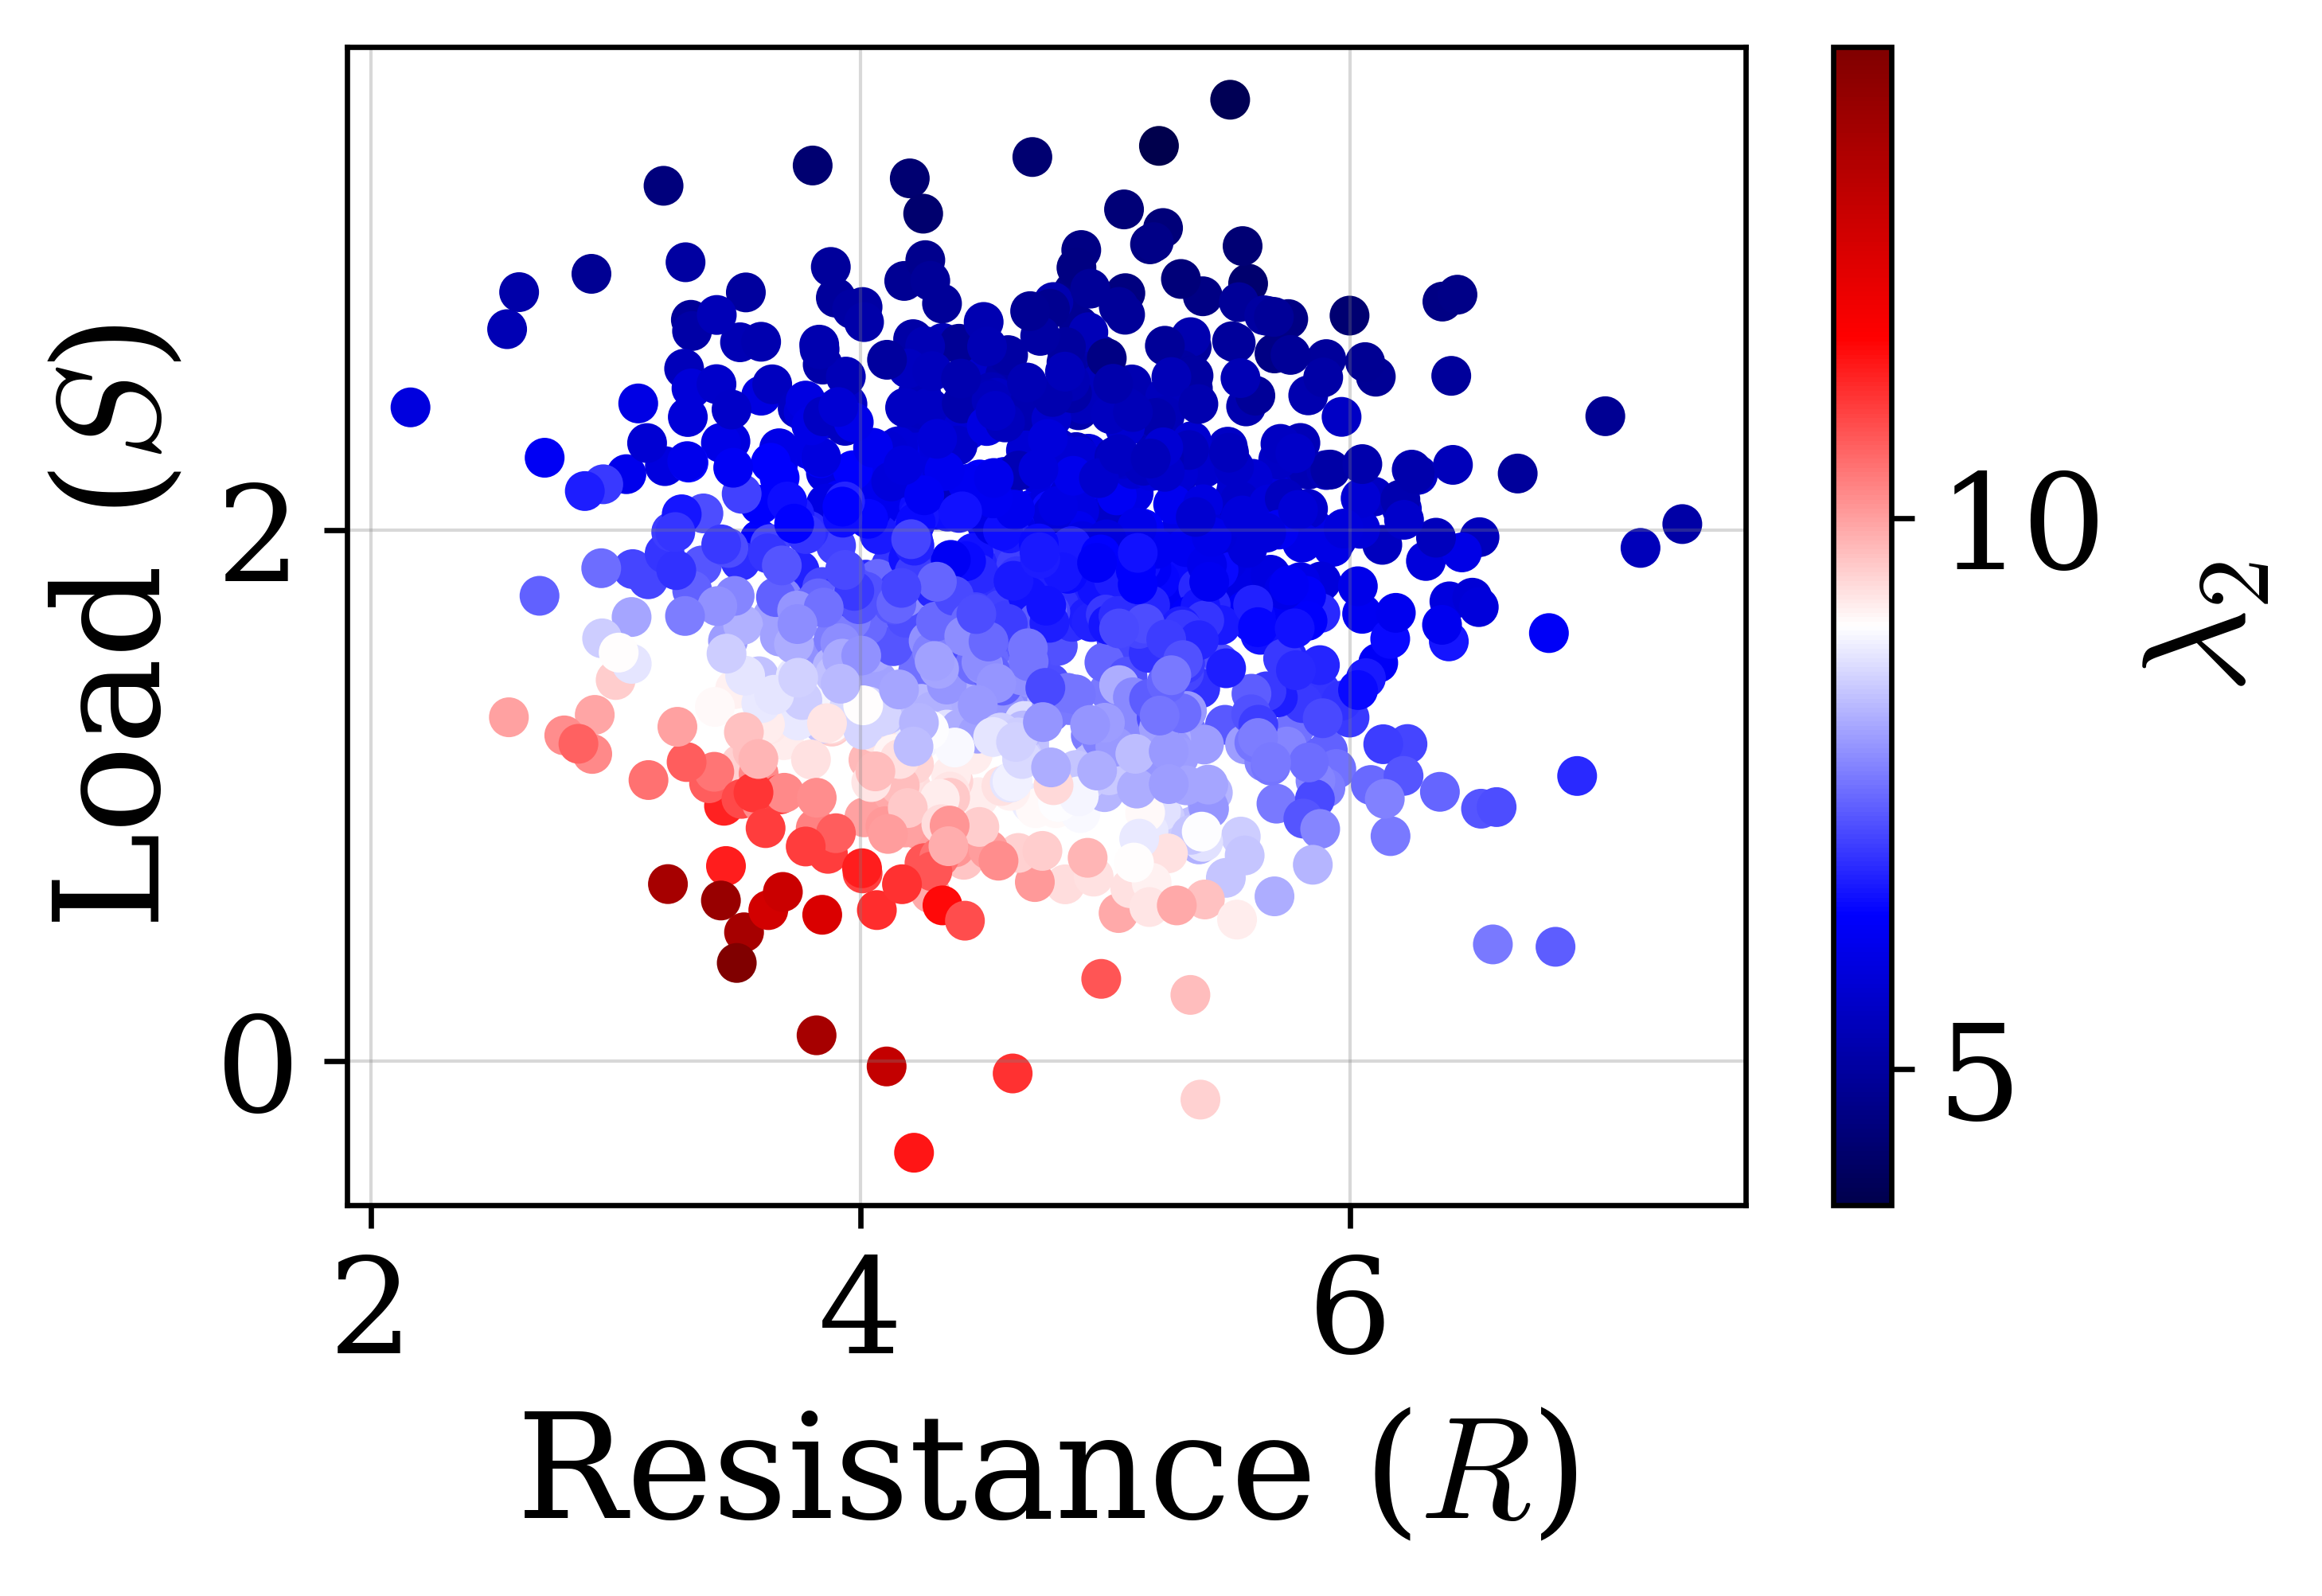
\includegraphics[
            width=\textwidth,
            height=0.667\textwidth,
            keepaspectratio
        ]{z_lambda_2_t-0.png}
        \caption{$\lambda_2$ ($t=0$)}
    \end{subfigure}
    \hfill
    \begin{subfigure}[b]{0.24\textwidth}
        \centering
        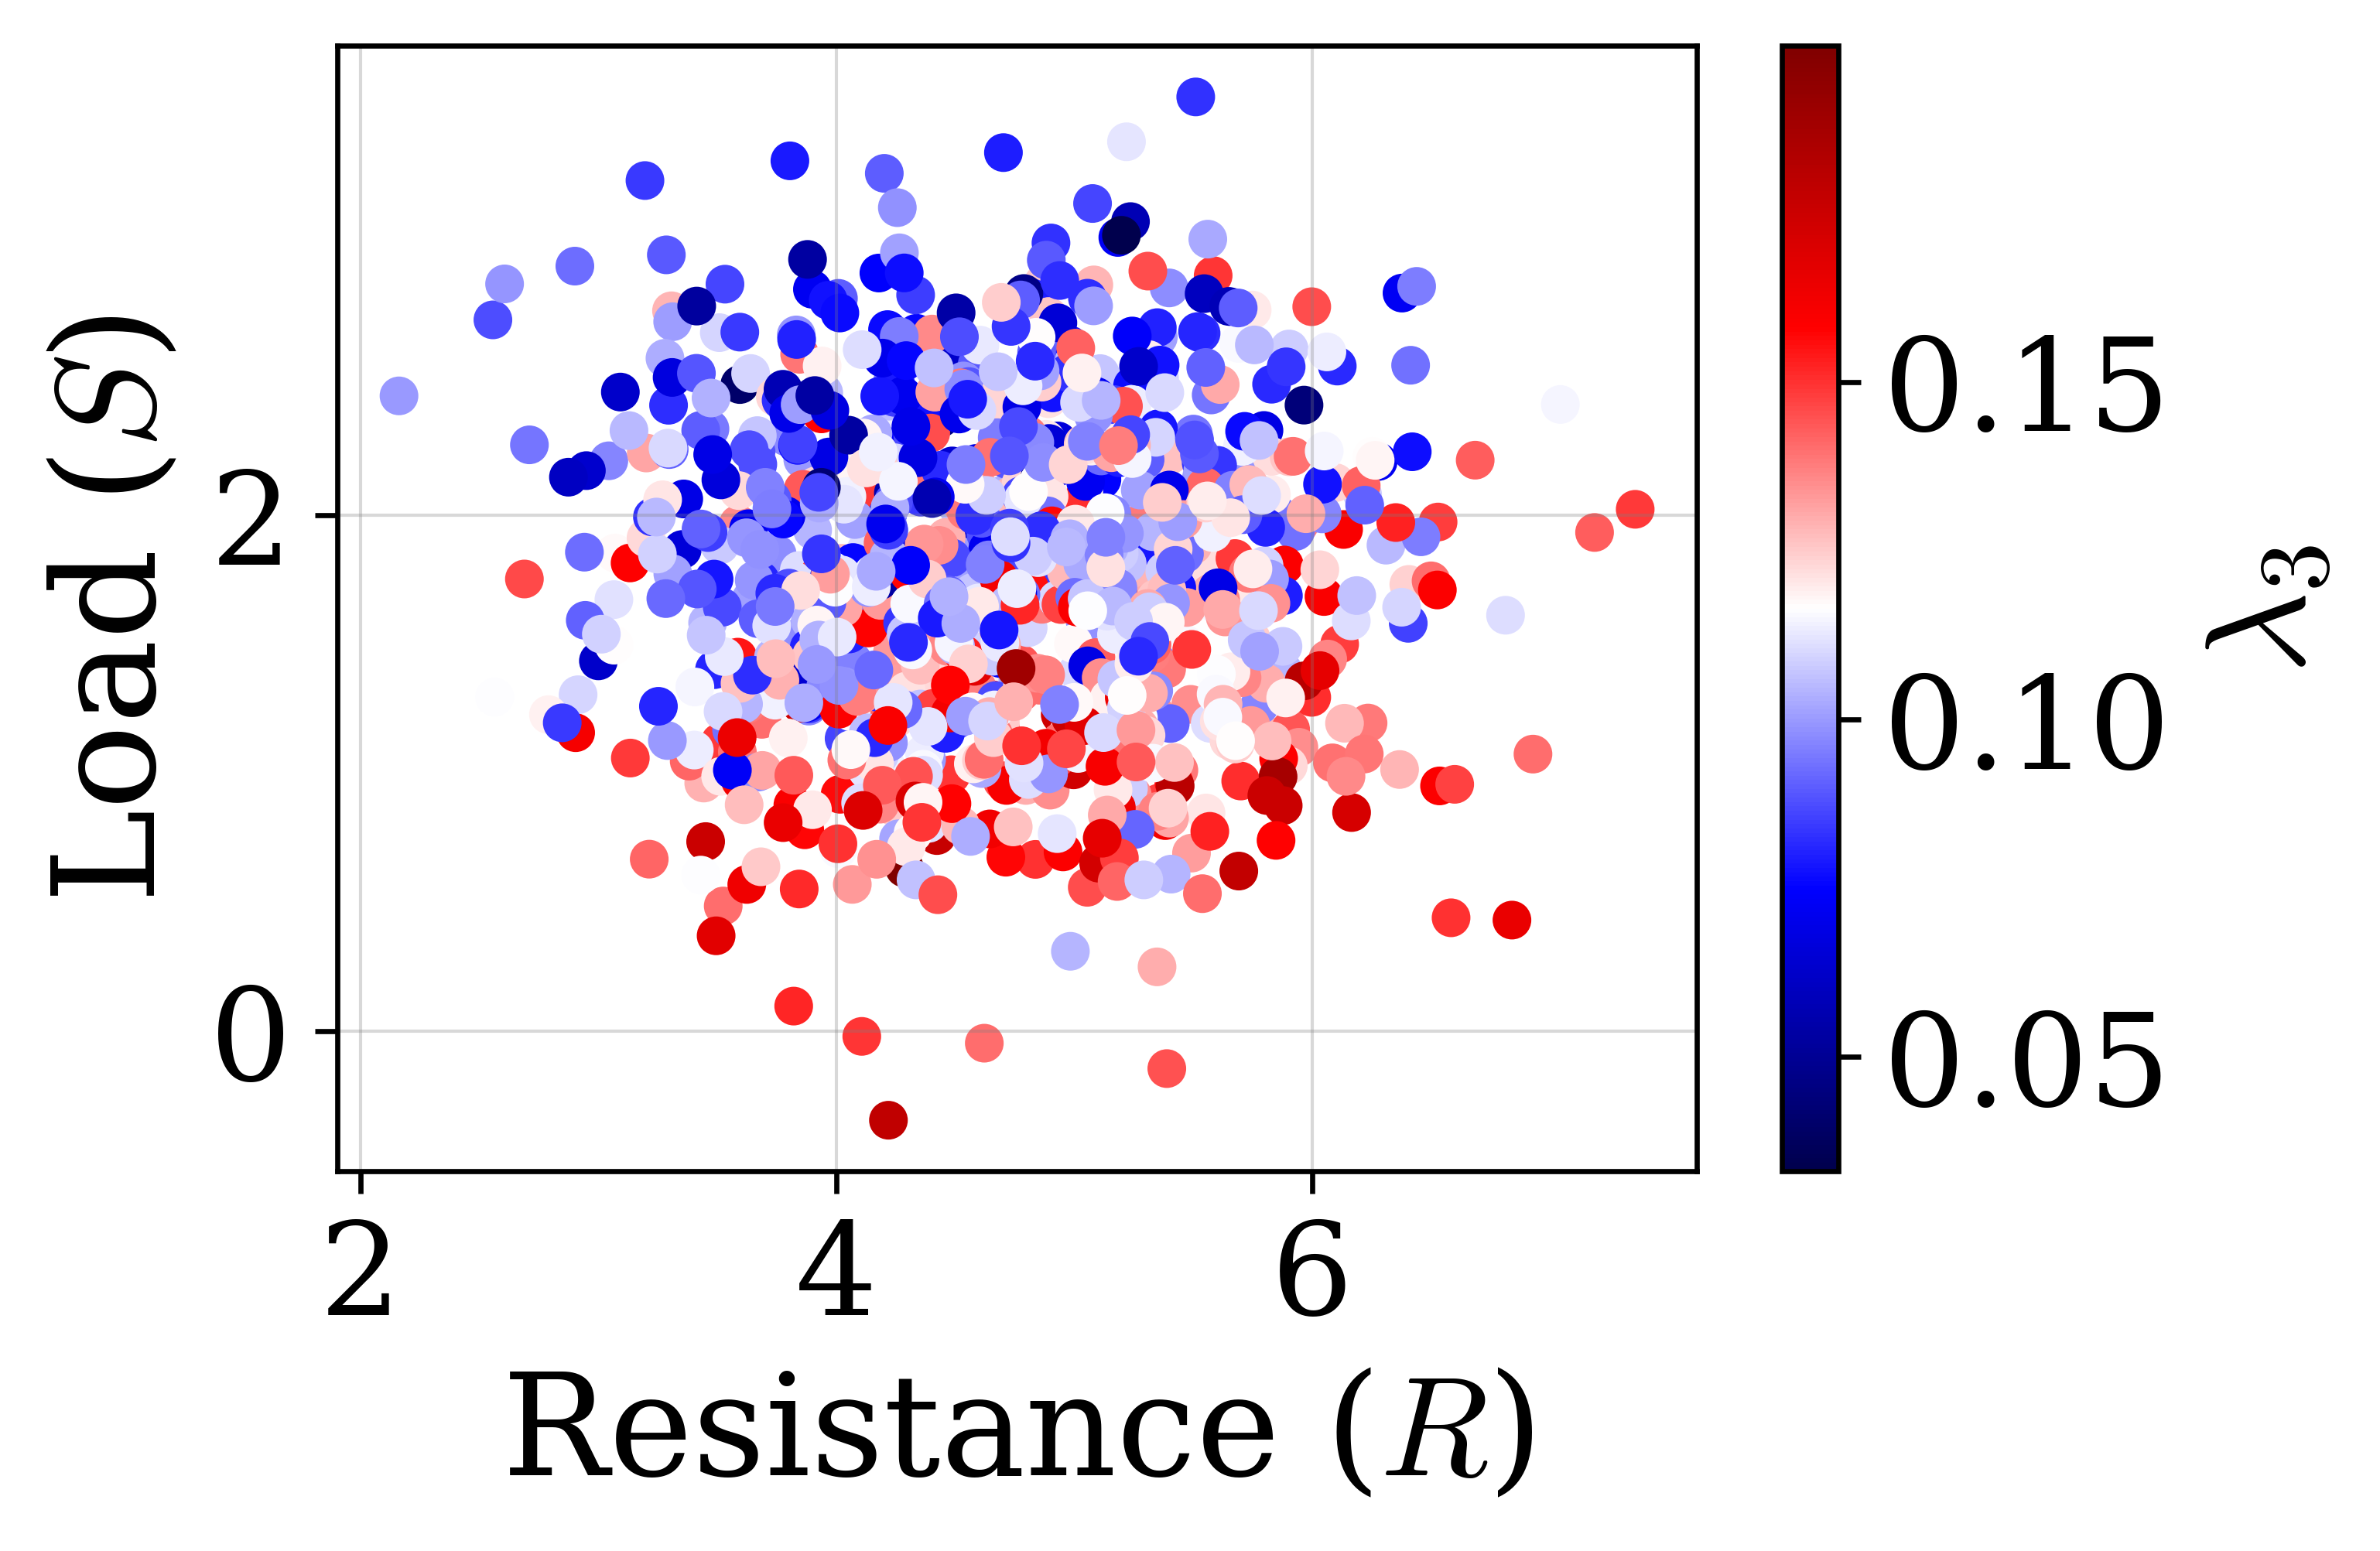
\includegraphics[
            width=\textwidth,
            height=0.667\textwidth,
            keepaspectratio
        ]{z_lambda_3_t-0.png}
        \caption{$\lambda_3$ ($t=0$)}
    \end{subfigure}
    \hfill
    \begin{subfigure}[b]{0.24\textwidth}
        \centering
        
\includegraphics[
            width=\textwidth,
            height=0.667\textwidth,
            keepaspectratio
        ]{z_lambda_4_t-0.png}
        \caption{$\lambda_4$ ($t=0$)}
    \end{subfigure}

    \par\bigskip

    % --- LINHA 2 (Tempo t=50) ---
    \begin{subfigure}[b]{0.24\textwidth}
        \centering
        
\includegraphics[
            width=\textwidth,
            height=0.667\textwidth,
            keepaspectratio
        ]{z_lambda_1_t-50.png}
        \caption{$\lambda_1$ ($t=50$)}
    \end{subfigure}
    \hfill
    \begin{subfigure}[b]{0.24\textwidth}
        \centering
        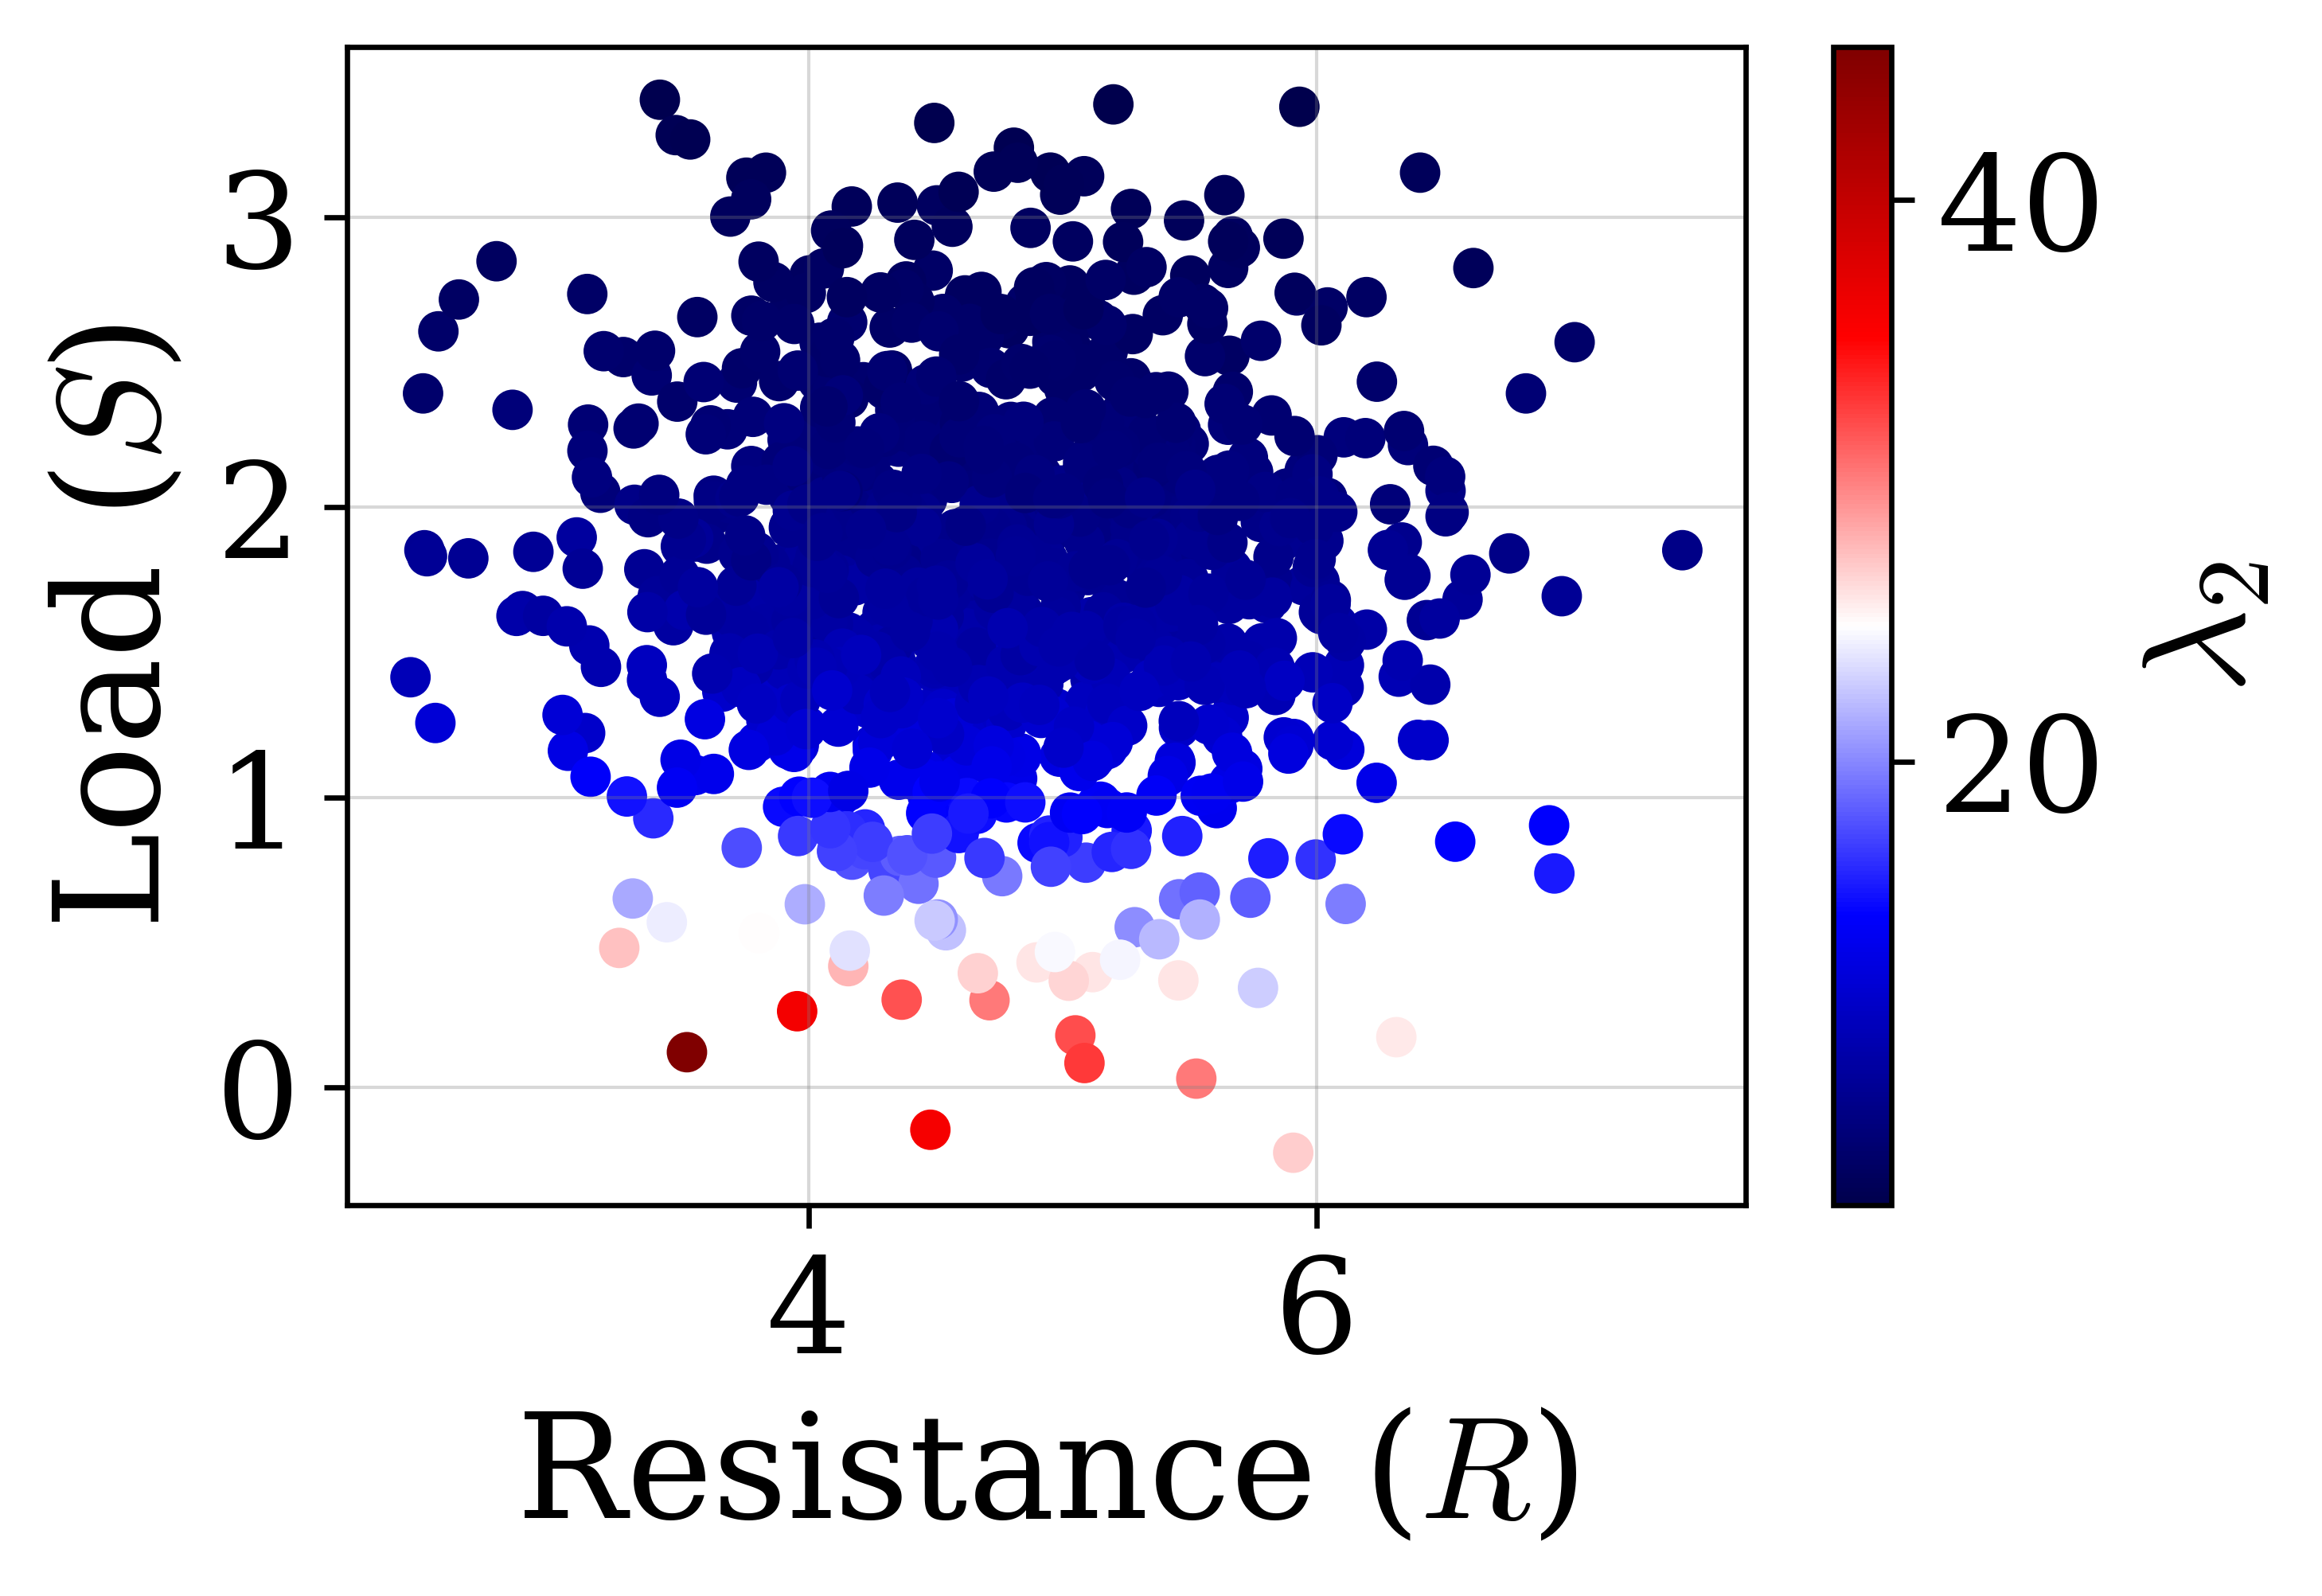
\includegraphics[
            width=\textwidth,
            height=0.667\textwidth,
            keepaspectratio
        ]{z_lambda_2_t-50.png}
        \caption{$\lambda_2$ ($t=50$)}
    \end{subfigure}
    \hfill
    \begin{subfigure}[b]{0.24\textwidth}
        \centering
        
\includegraphics[
            width=\textwidth,
            height=0.667\textwidth,
            keepaspectratio
        ]{z_lambda_3_t-50.png}
        \caption{$\lambda_3$ ($t=50$)}
    \end{subfigure}
    \hfill
    \begin{subfigure}[b]{0.24\textwidth}
        \centering
        
\includegraphics[
            width=\textwidth,
            height=0.667\textwidth,
            keepaspectratio
        ]{z_lambda_4_t-50.png}
        \caption{$\lambda_4$ ($t=50$)}
    \end{subfigure}

    \caption{Scatter plots of \textbf{R} and \textbf{S} realizations for GLAM parameters $\lambda_1$--$\lambda_4$ at $t=0$ and $t=50$.}
    \label{fig:toy_lambda_scatter_grid}
\end{figure}

%Assim ,é possível perceber que os valore de lamda 1 e 2 são sensíveis, enquanto 3 e 4 não alteram significativamente escala de alteração baixa. Isso corrobora a hiptese de não treinar 3 e 4. assim foi feito o treinamento com o seguinte resultado:

Based on this evidence, only $\lambda_1$ and $\lambda_2$ are selected as target variables for the surrogate model training. The performance of the resulting PCE metamodel is evaluated through the coefficient of determination, $R^2$, and the validation results are reported in Table~\ref{tab:validation_results}. The high $R^2$ values obtained for $\lambda_1$ and $\lambda_2$ across all time steps indicate excellent predictive accuracy, while the consistently low $R^2$ values for $\lambda_3$ and $\lambda_4$ further confirm their limited variability and support their exclusion from the training process.

\begin{table}[H]
\centering
\caption{Statistical validation results of the PCE metamodel at different time steps.}
\label{tab:validation_results}
\begin{tabular}{rrrrr}
\toprule
Time & $R^2$ ($\lambda_1$) & $R^2$ ($\lambda_2$) & $R^2$ ($\lambda_3$) & $R^2$ ($\lambda_4$) \\
\midrule
0 & 1.0000 & 0.9839 & 0.3858 & 0.3978 \\
10 & 1.0000 & 0.9887 & 0.4448 & 0.4226 \\
20 & 1.0000 & 0.9894 & 0.3713 & 0.3804 \\
30 & 1.0000 & 0.9833 & 0.3758 & 0.3624 \\
40 & 1.0000 & 0.9792 & 0.4081 & 0.3891 \\
50 & 1.0000 & 0.9908 & 0.3293 & 0.3757 \\
60 & 1.0000 & 0.9926 & 0.3102 & 0.3525 \\
70 & 1.0000 & 0.9853 & 0.2266 & 0.2852 \\
80 & 1.0000 & 0.9918 & 0.2277 & 0.2146 \\
90 & 1.0000 & 0.9820 & 0.1536 & 0.2200 \\
100 & 1.0000 & 0.9865 & 0.0638 & 0.1352 \\
\bottomrule
\end{tabular}
\end{table}

For the fixed realizations $r = 5.09$ and $s = 1.80$, four Polynomial Chaos Expansion (PCE) models were trained. Figure~\ref{fig:kde_comparison} presents the Kernel Density Estimation (KDE) comparison between the Ground Truth and the GLAM approximation obtained via PCE. For each realization, the GLAM–PCE response was evaluated and plotted at two distinct time periods, namely $t = 0$ and $t = 50$, allowing the assessment of the model’s ability to reproduce the probabilistic behavior of the reference solution over time.

\begin{figure}[H]
    \centering
    % --- Coluna 1: Tempo t=0 ---
    \begin{subfigure}[b]{0.38\textwidth}
        \centering
        % Substitua pelo nome do seu arquivo
        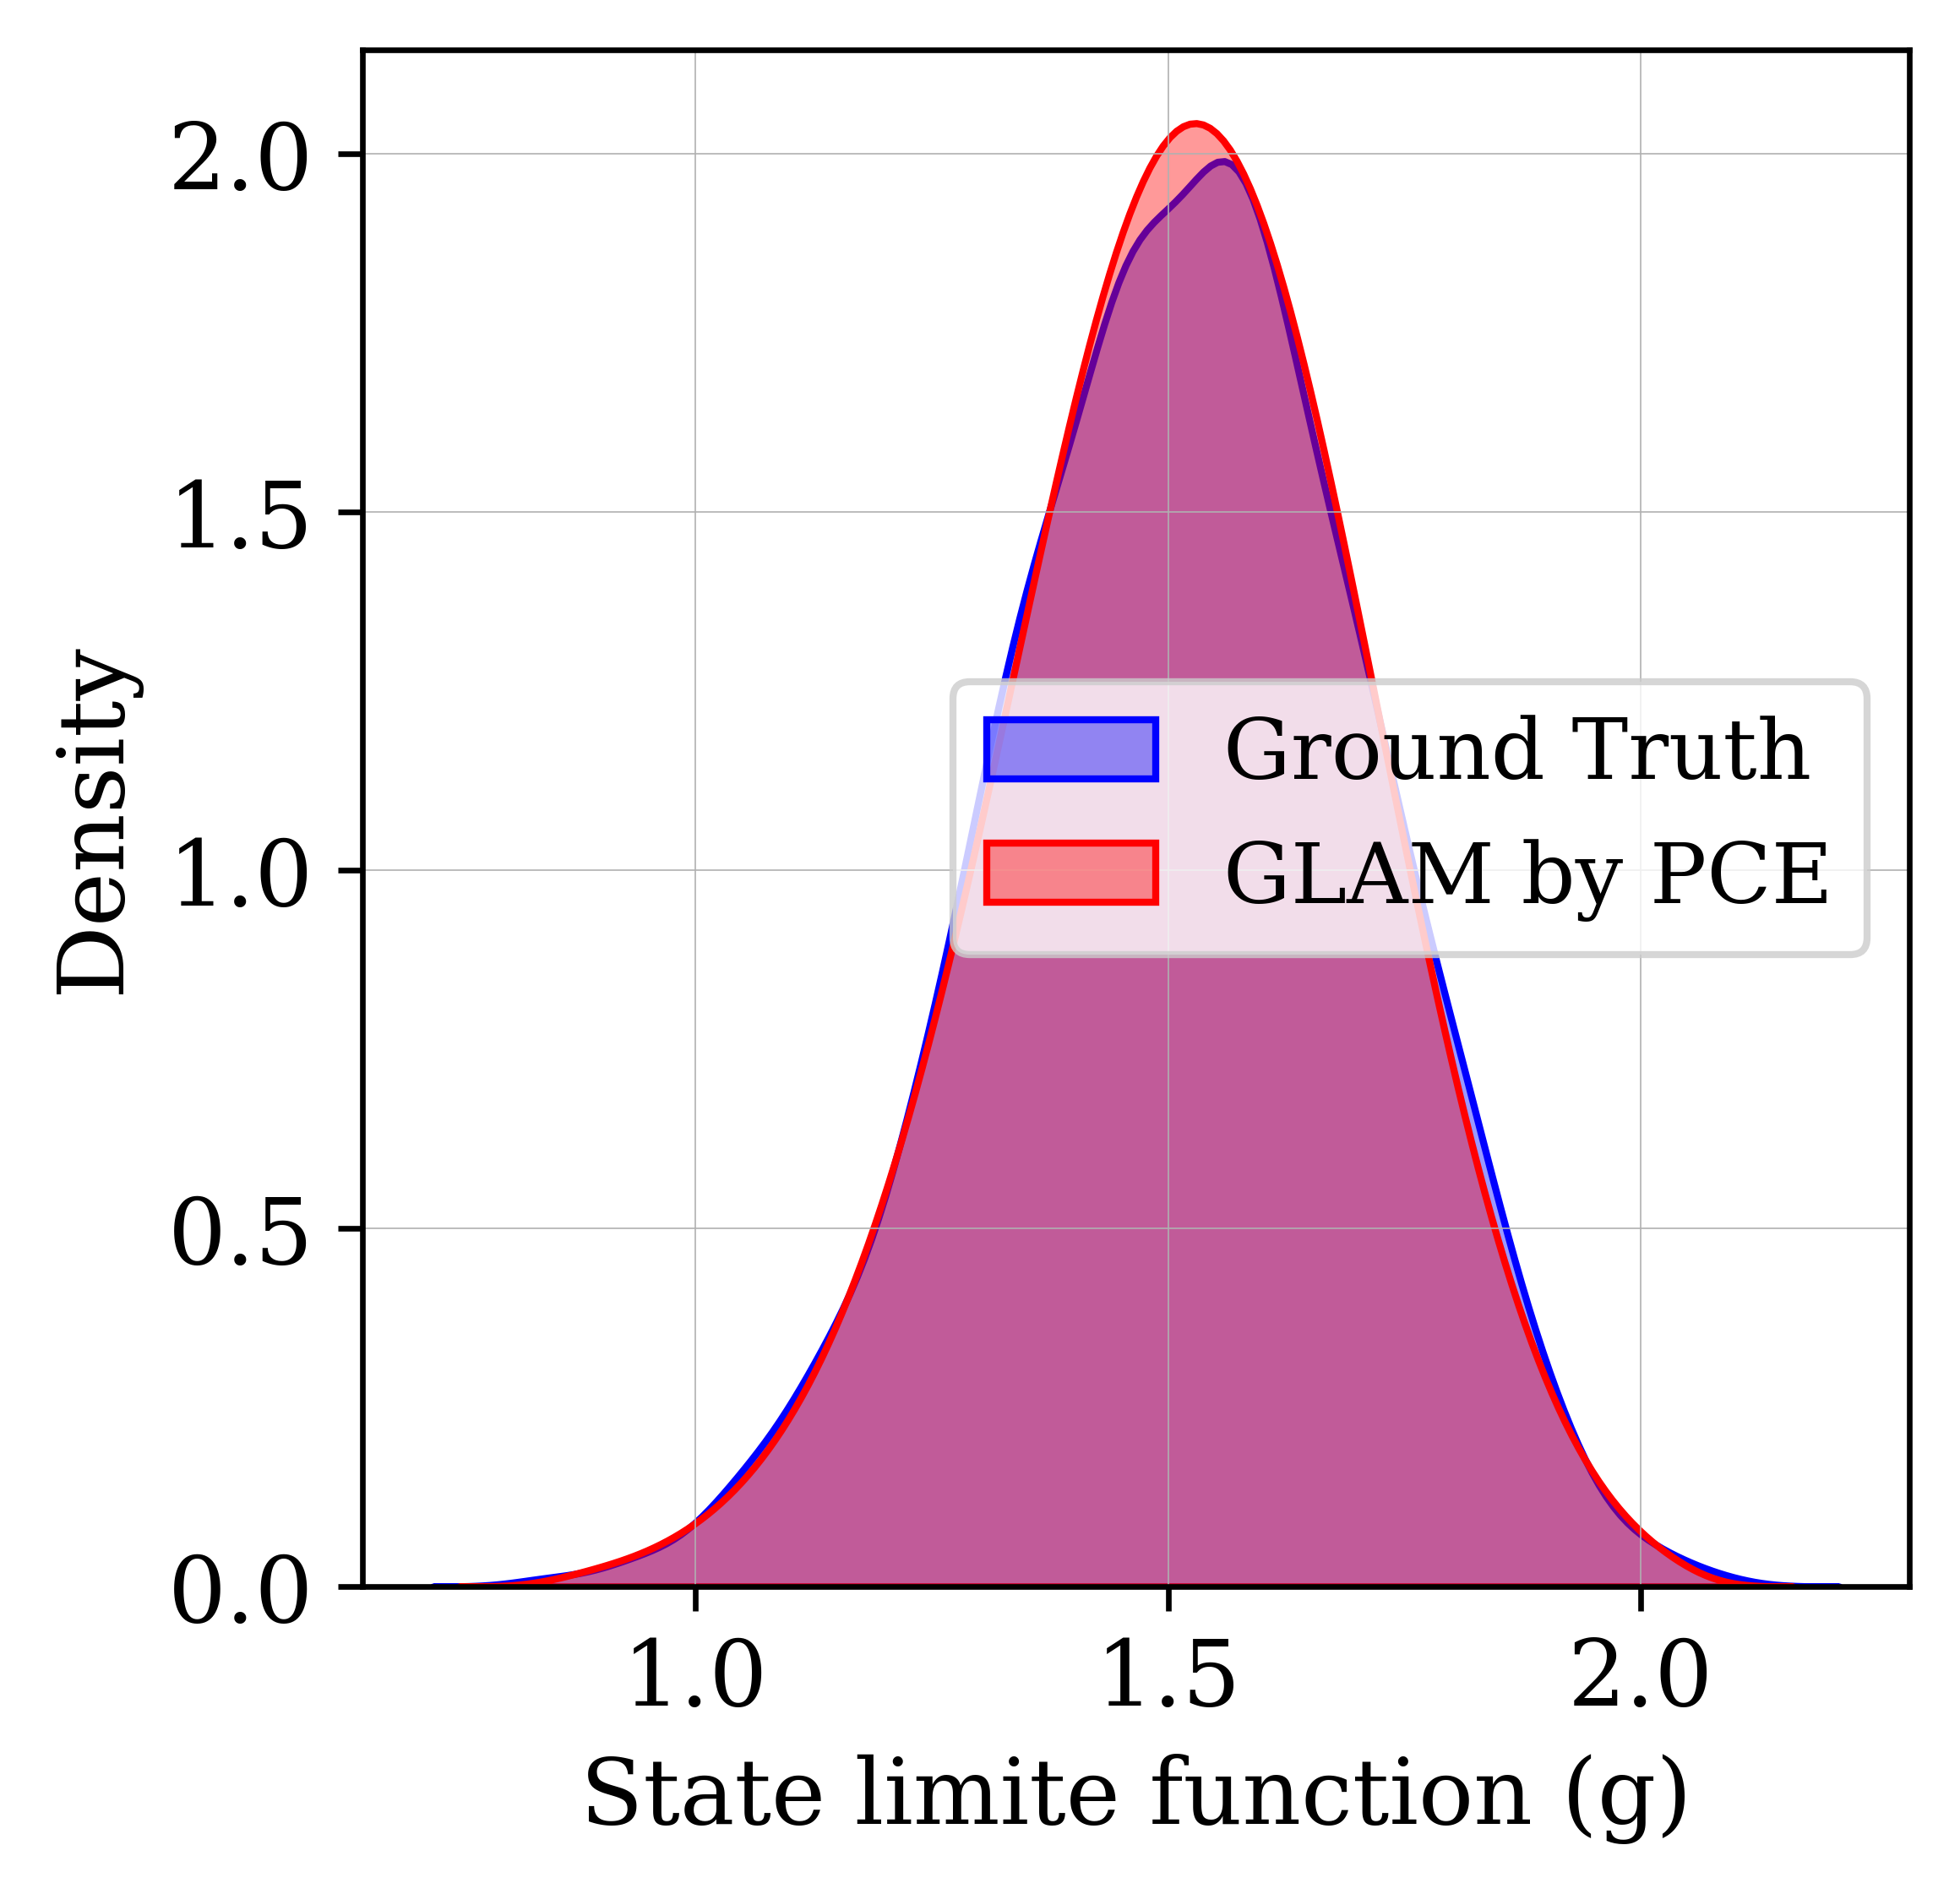
\includegraphics[width=\textwidth]{z_histogram_glam_versus_gt_t0_en.png}
        \caption{Time $t=0$}
        \label{fig:kde_t0}
    \end{subfigure}
    \hfill % O hfill empurra uma figura para a esquerda e outra para a direita
    % --- Coluna 2: Tempo t=50 ---
    \begin{subfigure}[b]{0.38\textwidth}
        \centering
        % Substitua pelo nome do seu arquivo
        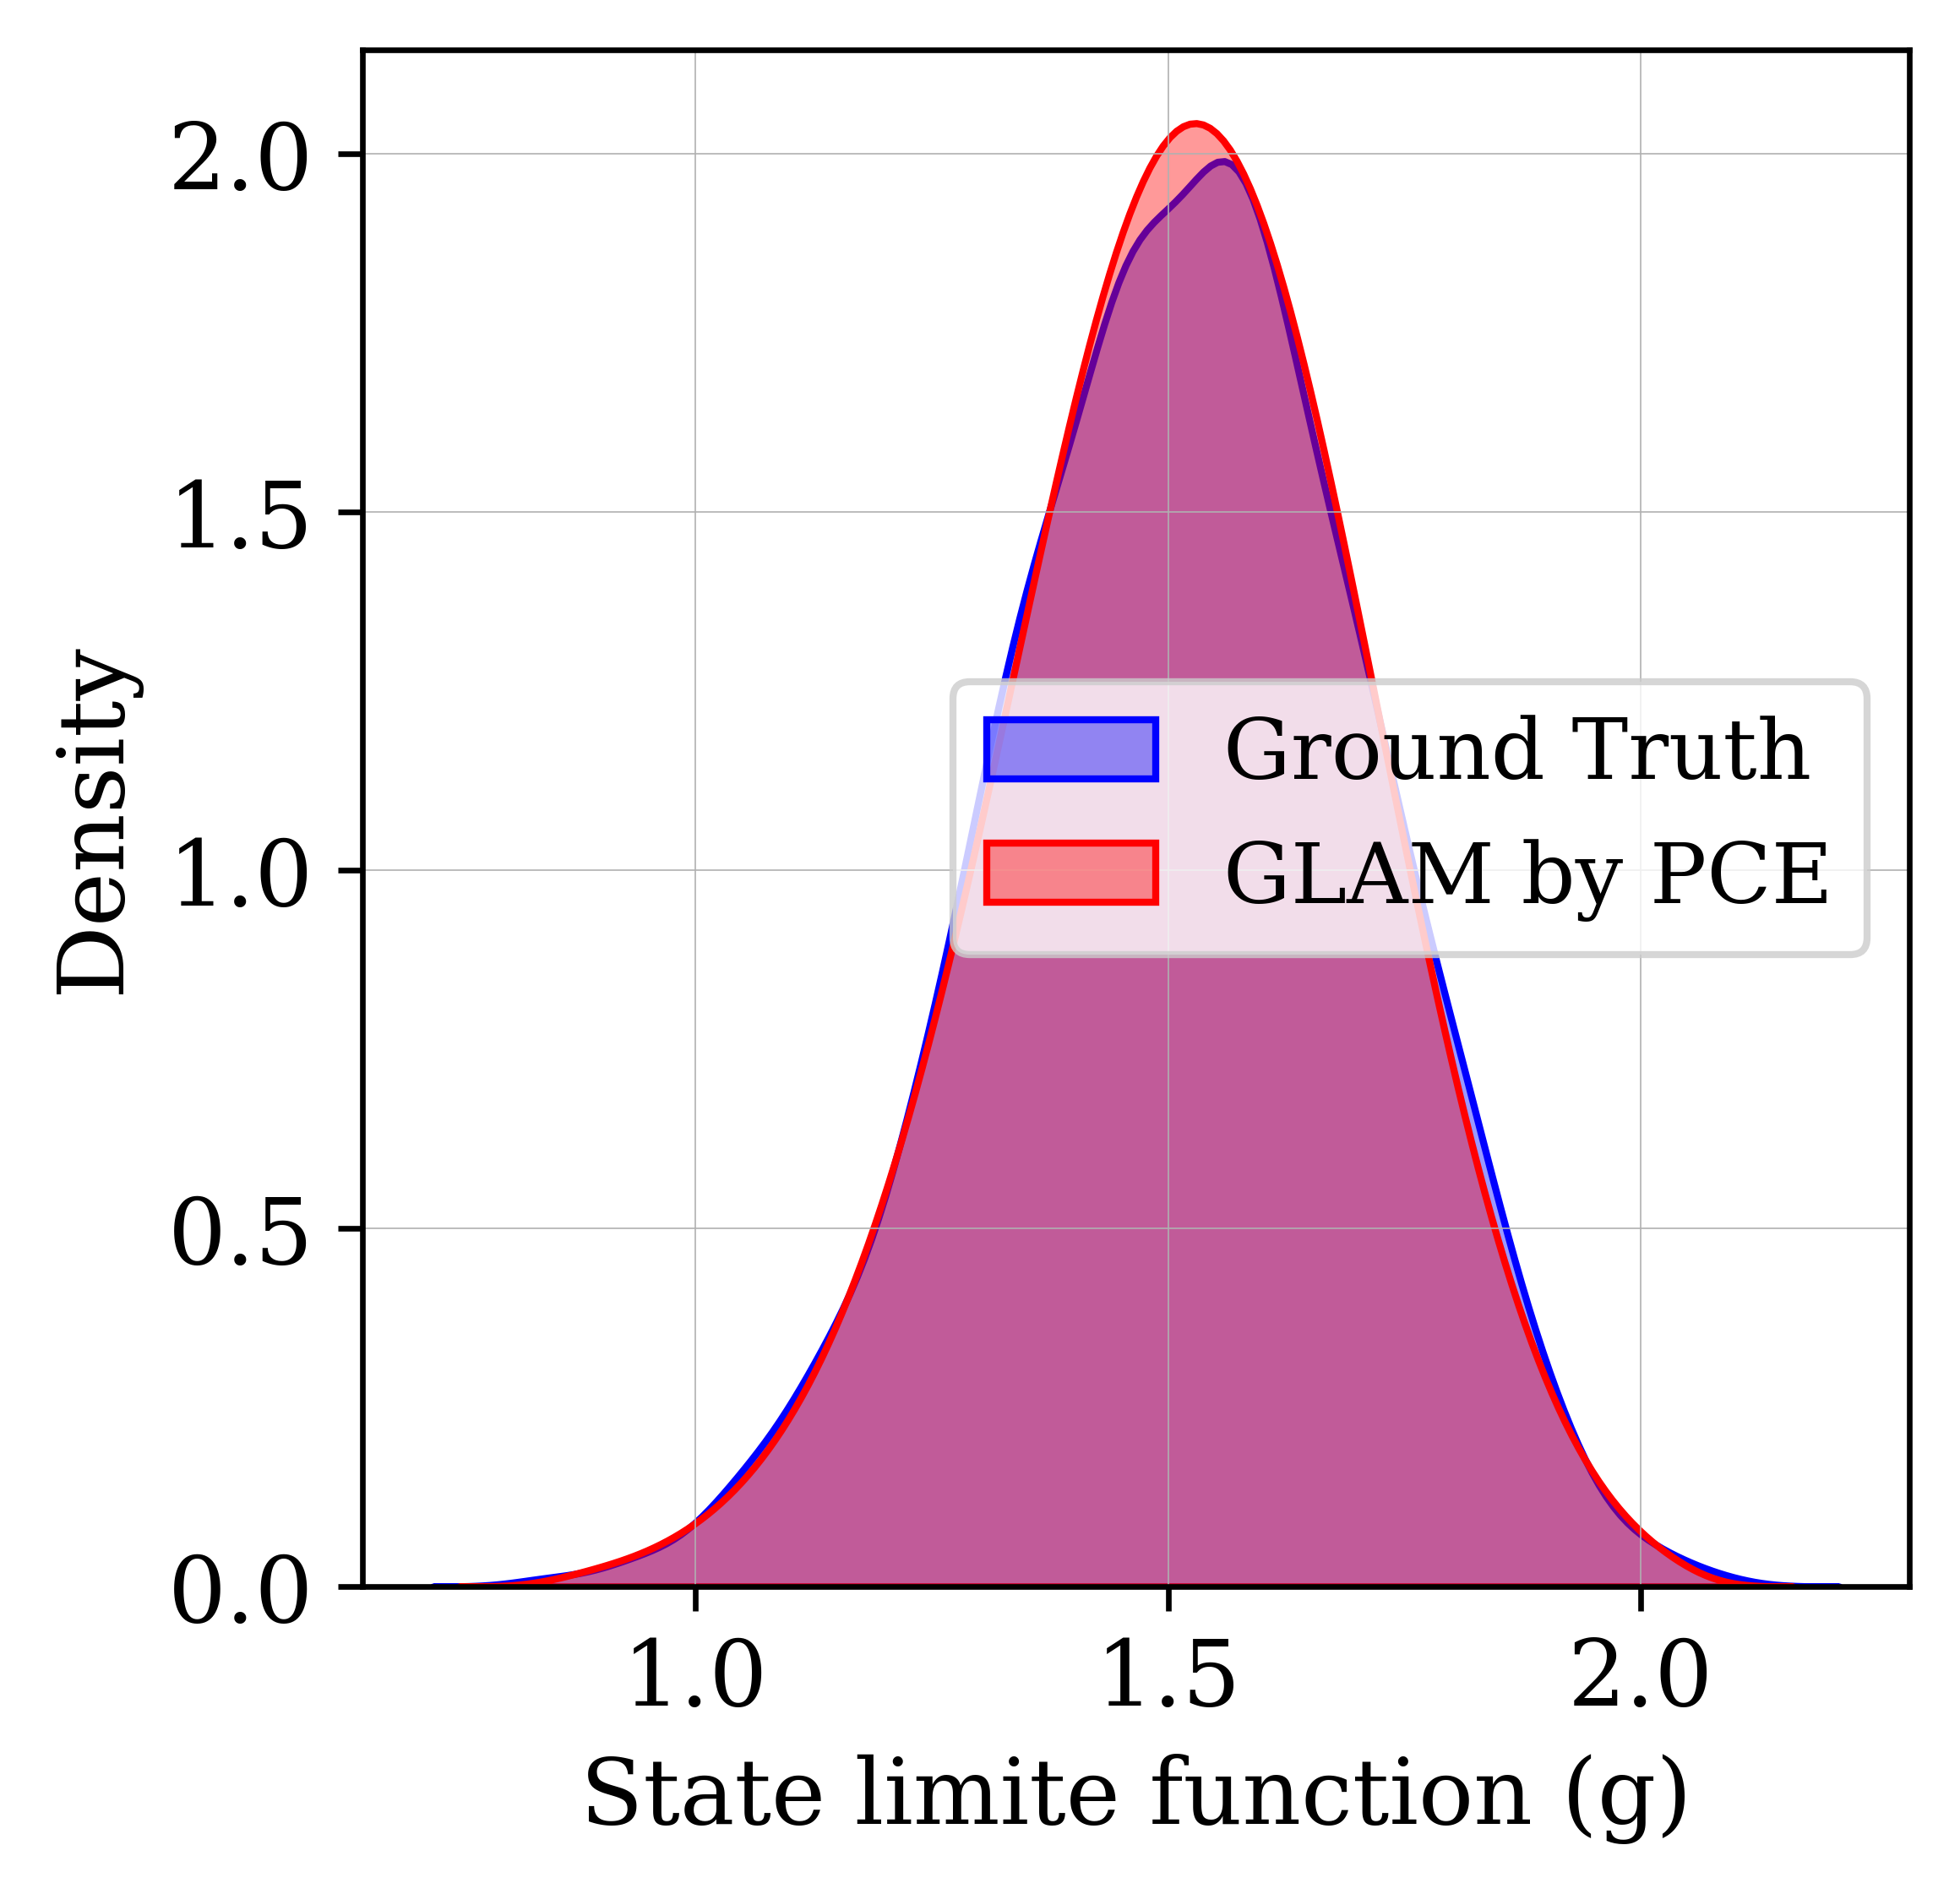
\includegraphics[width=\textwidth]{z_histogram_glam_versus_gt_t50_en.png}
        \caption{Time $t=50$}
        \label{fig:kde_t50}
    \end{subfigure}
    \caption{Comparison between Ground Truth and GLAM approximation using KDE. PCE models for the fixed realizations $r=5.09$ and $s=1.80$.}
    \label{fig:kde_comparison}
\end{figure}

The statistical similarity between the reference data (GT) and the values generated by the metamodel (GLAM) was assessed using non-parametric goodness-of-fit tests and quantile-based comparisons. Tables~\ref{tab:statistical_tests} and~\ref{tab:quantile_comparison} summarize the results of the hypothesis tests and the quantile comparison, respectively.

\begin{table}[H]
\centering
\caption{Results of the Kolmogorov--Smirnov and Anderson--Darling statistical tests for comparison between the reference data (GT) and the metamodel predictions (GLAM).}
\label{tab:statistical_tests}
\begin{tabular}{lcccc}
\hline
Test & Statistic & p-value & Significance level ($\alpha$) & Decision \\
\hline
Kolmogorov--Smirnov & 0.0108 & 0.9325 & 0.05 & Fail to reject $H_0$ \\
Anderson--Darling  & -0.6492 & 0.0025 & 0.05 & Reject $H_0$ \\
\hline
\end{tabular}
\end{table}

As shown in Table~\ref{tab:statistical_tests}, the Kolmogorov--Smirnov (KS) test does not reject the null hypothesis at the 5\% significance level, yielding a maximum distance of $D = 0.0108$. This result indicates an excellent global agreement between the empirical cumulative distribution functions of the reference data and the metamodel predictions. The KS test is primarily sensitive to the maximum discrepancy over the entire support of the distribution, making it well suited for assessing overall distributional similarity \cite{massey1951ks}.

In contrast, the Anderson--Darling (AD) test rejects the null hypothesis, indicating statistically significant differences between the samples. This outcome is attributed to the higher sensitivity of the AD test to discrepancies in the tails of the distribution, particularly in the presence of large sample sizes \cite{anderson1952ad, scholz1987ad}. Such behavior is well documented in the literature and does not necessarily imply poor global agreement between distributions.

To further investigate the origin of the discrepancy identified by the Anderson--Darling test, a quantile-based comparison was performed. The results are presented in Table~\ref{tab:quantile_comparison}.

\begin{table}[H]
\centering
\caption{Quantile comparison between the reference data (GT) and the metamodel predictions (GLAM).}
\label{tab:quantile_comparison}
\begin{tabular}{ccccc}
\hline
Quantile & GT & GLAM & Absolute difference & Relative difference (\%) \\
\hline
0.001 & 0.8995 & 0.9037 & 0.0042 & 0.47 \\
0.010 & 1.0387 & 1.0393 & 0.0006 & 0.06 \\
0.500 & 1.5222 & 1.5198 & 0.0024 & 0.16 \\
0.990 & 1.9374 & 1.9356 & 0.0018 & 0.09 \\
0.999 & 2.0529 & 2.0263 & 0.0266 & 1.30 \\
\hline
\end{tabular}
\end{table}

The quantile analysis reported in Table~\ref{tab:quantile_comparison} confirms the excellent agreement between the two datasets across nearly the entire distribution. Relative differences remain below 0.1\% up to the 99th percentile, indicating that the metamodel accurately reproduces the central and moderately extreme regions of the distribution. At the extreme quantile of 99.9\%, the relative discrepancy increases to approximately 1.3\%, which explains the rejection observed in the Anderson--Darling test due to its strong emphasis on tail behavior.

Overall, the combined evidence from the KS test, the AD test, and the quantile-based comparison demonstrates that the metamodel provides an accurate representation of the global distribution of the limit-state function, with only minor discrepancies confined to the extreme tails. Such discrepancies are commonly observed in surrogate-based modeling approaches and are generally considered acceptable in reliability and uncertainty quantification analyses, particularly when the primary interest lies in the global probabilistic response \cite{derkiureghian2009uq, sudret2008pce}.

In addition to the accuracy of the probabilistic predictions, the proposed emulator-based framework offers a substantial gain in computational efficiency. Table~\ref{tab:computational_time} compares the computational time required by the conventional approach and the surrogate-based emulator for the considered example. While the conventional procedure required approximately $48.75$ seconds, the emulator reduced the computational cost to only $0.66$ seconds, corresponding to a speed-up of more than two orders of magnitude. This result highlights the suitability of the proposed approach for real-time or large-scale reliability and RUL analyses.

\begin{table}[H]
\centering
\caption{Comparison of computational time between the conventional approach and the emulator-based approach.}
\label{tab:computational_time}
\begin{tabular}{l c}
\hline
\textbf{Method} & \textbf{Computational Time (s)} \\
\hline
Conventional approach & 48.75 \\
Emulator-based approach & 0.66 \\
\hline
\end{tabular}
\end{table}

Figure~\ref{fig:rul_results} presents the probabilistic outputs of the surrogate-based framework employed for Remaining Useful Life (RUL) assessment within a structural health monitoring context. The results illustrate the propagation of uncertainty from the limit state response to the final RUL estimation.

Figure~\ref{fig:kde_inspection_time} shows the Kernel Density Estimation (KDE) of the limit state function evaluated at the inspection time of 35 years, adopted here as a representative example. This distribution characterizes the uncertainty associated with the system condition at the inspection instant, capturing both the inherent variability of the stochastic inputs and the approximation effects introduced by the surrogate model.

The probability density function of the time to failure is presented in Figure~\ref{fig:kde_time_to_failure}. This distribution is obtained by identifying the time instant at which the limit state function approaches zero, providing a probabilistic description of the system lifetime and enabling a reliability-based interpretation of failure occurrence.

Finally, Figure~\ref{fig:kde_rul} presents the resulting RUL distribution, computed as the difference between the estimated time to failure and the inspection time. This distribution consolidates the propagated uncertainties and represents the key outcome for predictive maintenance and risk-informed decision-making.

\begin{figure}[H]
    \centering

    \begin{subfigure}[b]{0.32\textwidth}
        \centering
        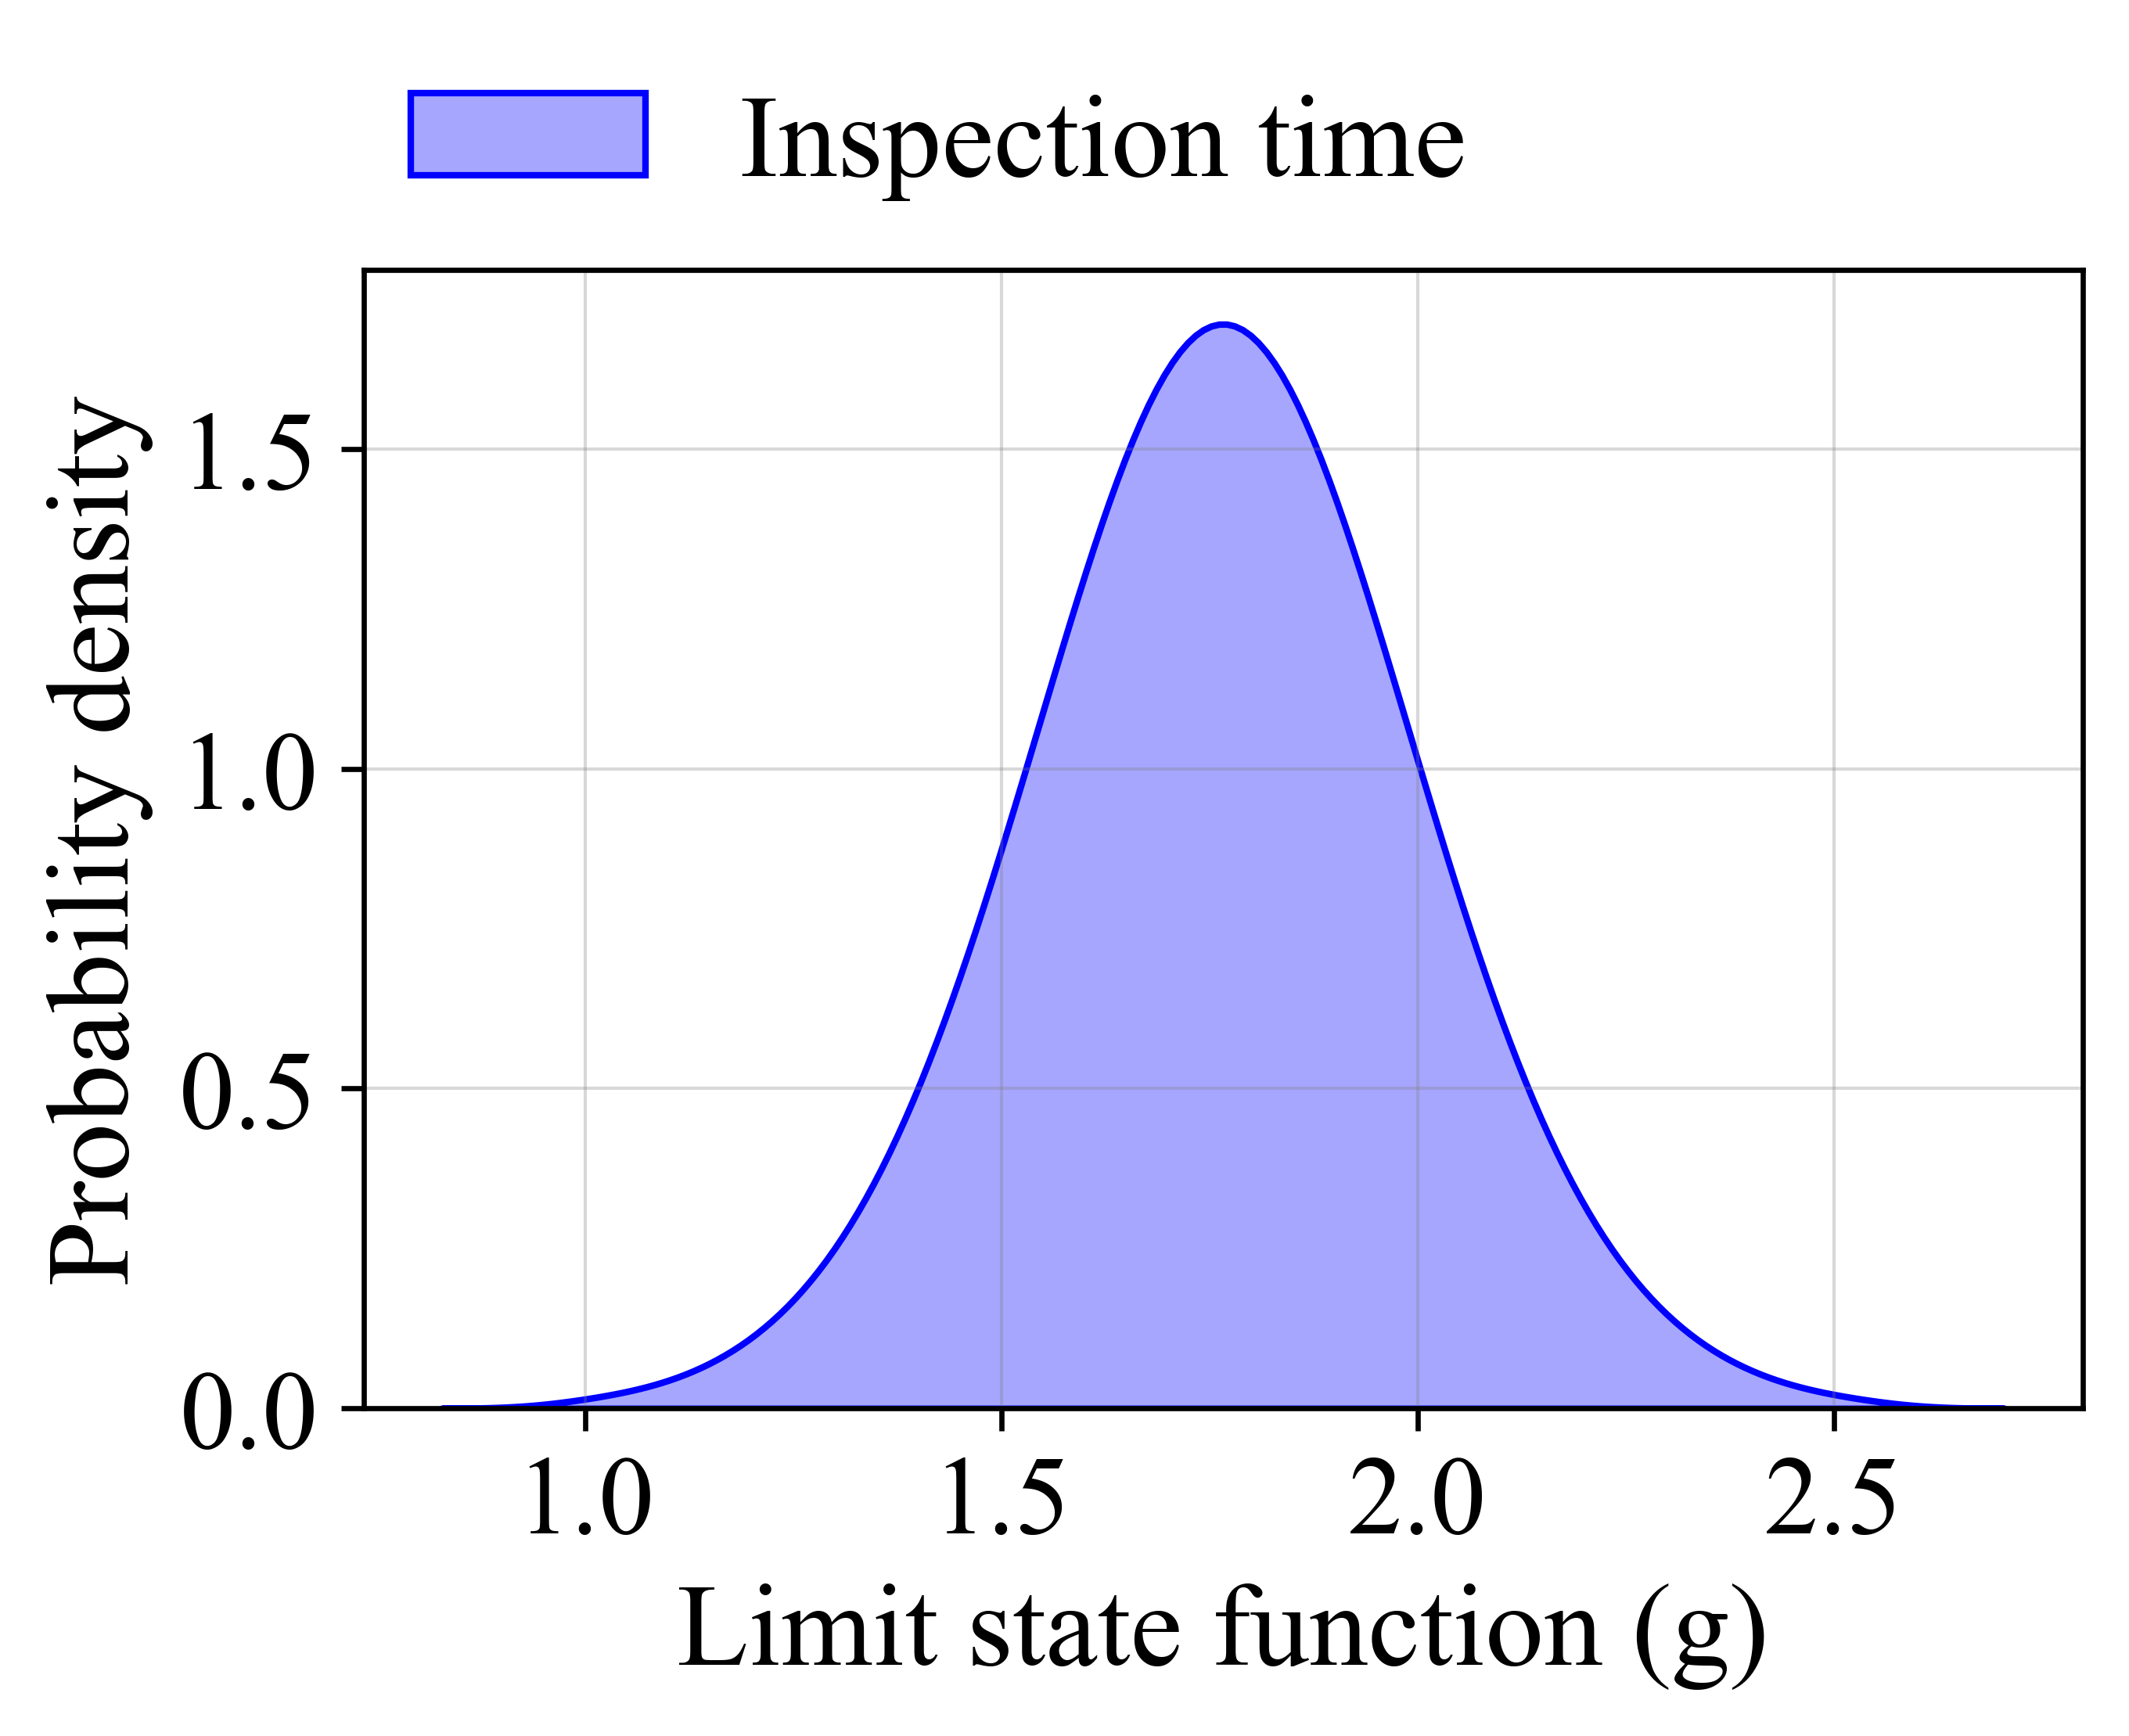
\includegraphics[
            height=4.0cm,
            keepaspectratio
        ]{z_kde_inspection_time.png}
        \caption{KDE of the limit state function at the inspection time.}
        \label{fig:kde_inspection_time}
    \end{subfigure}
    \hfill
    \begin{subfigure}[b]{0.32\textwidth}
        \centering
        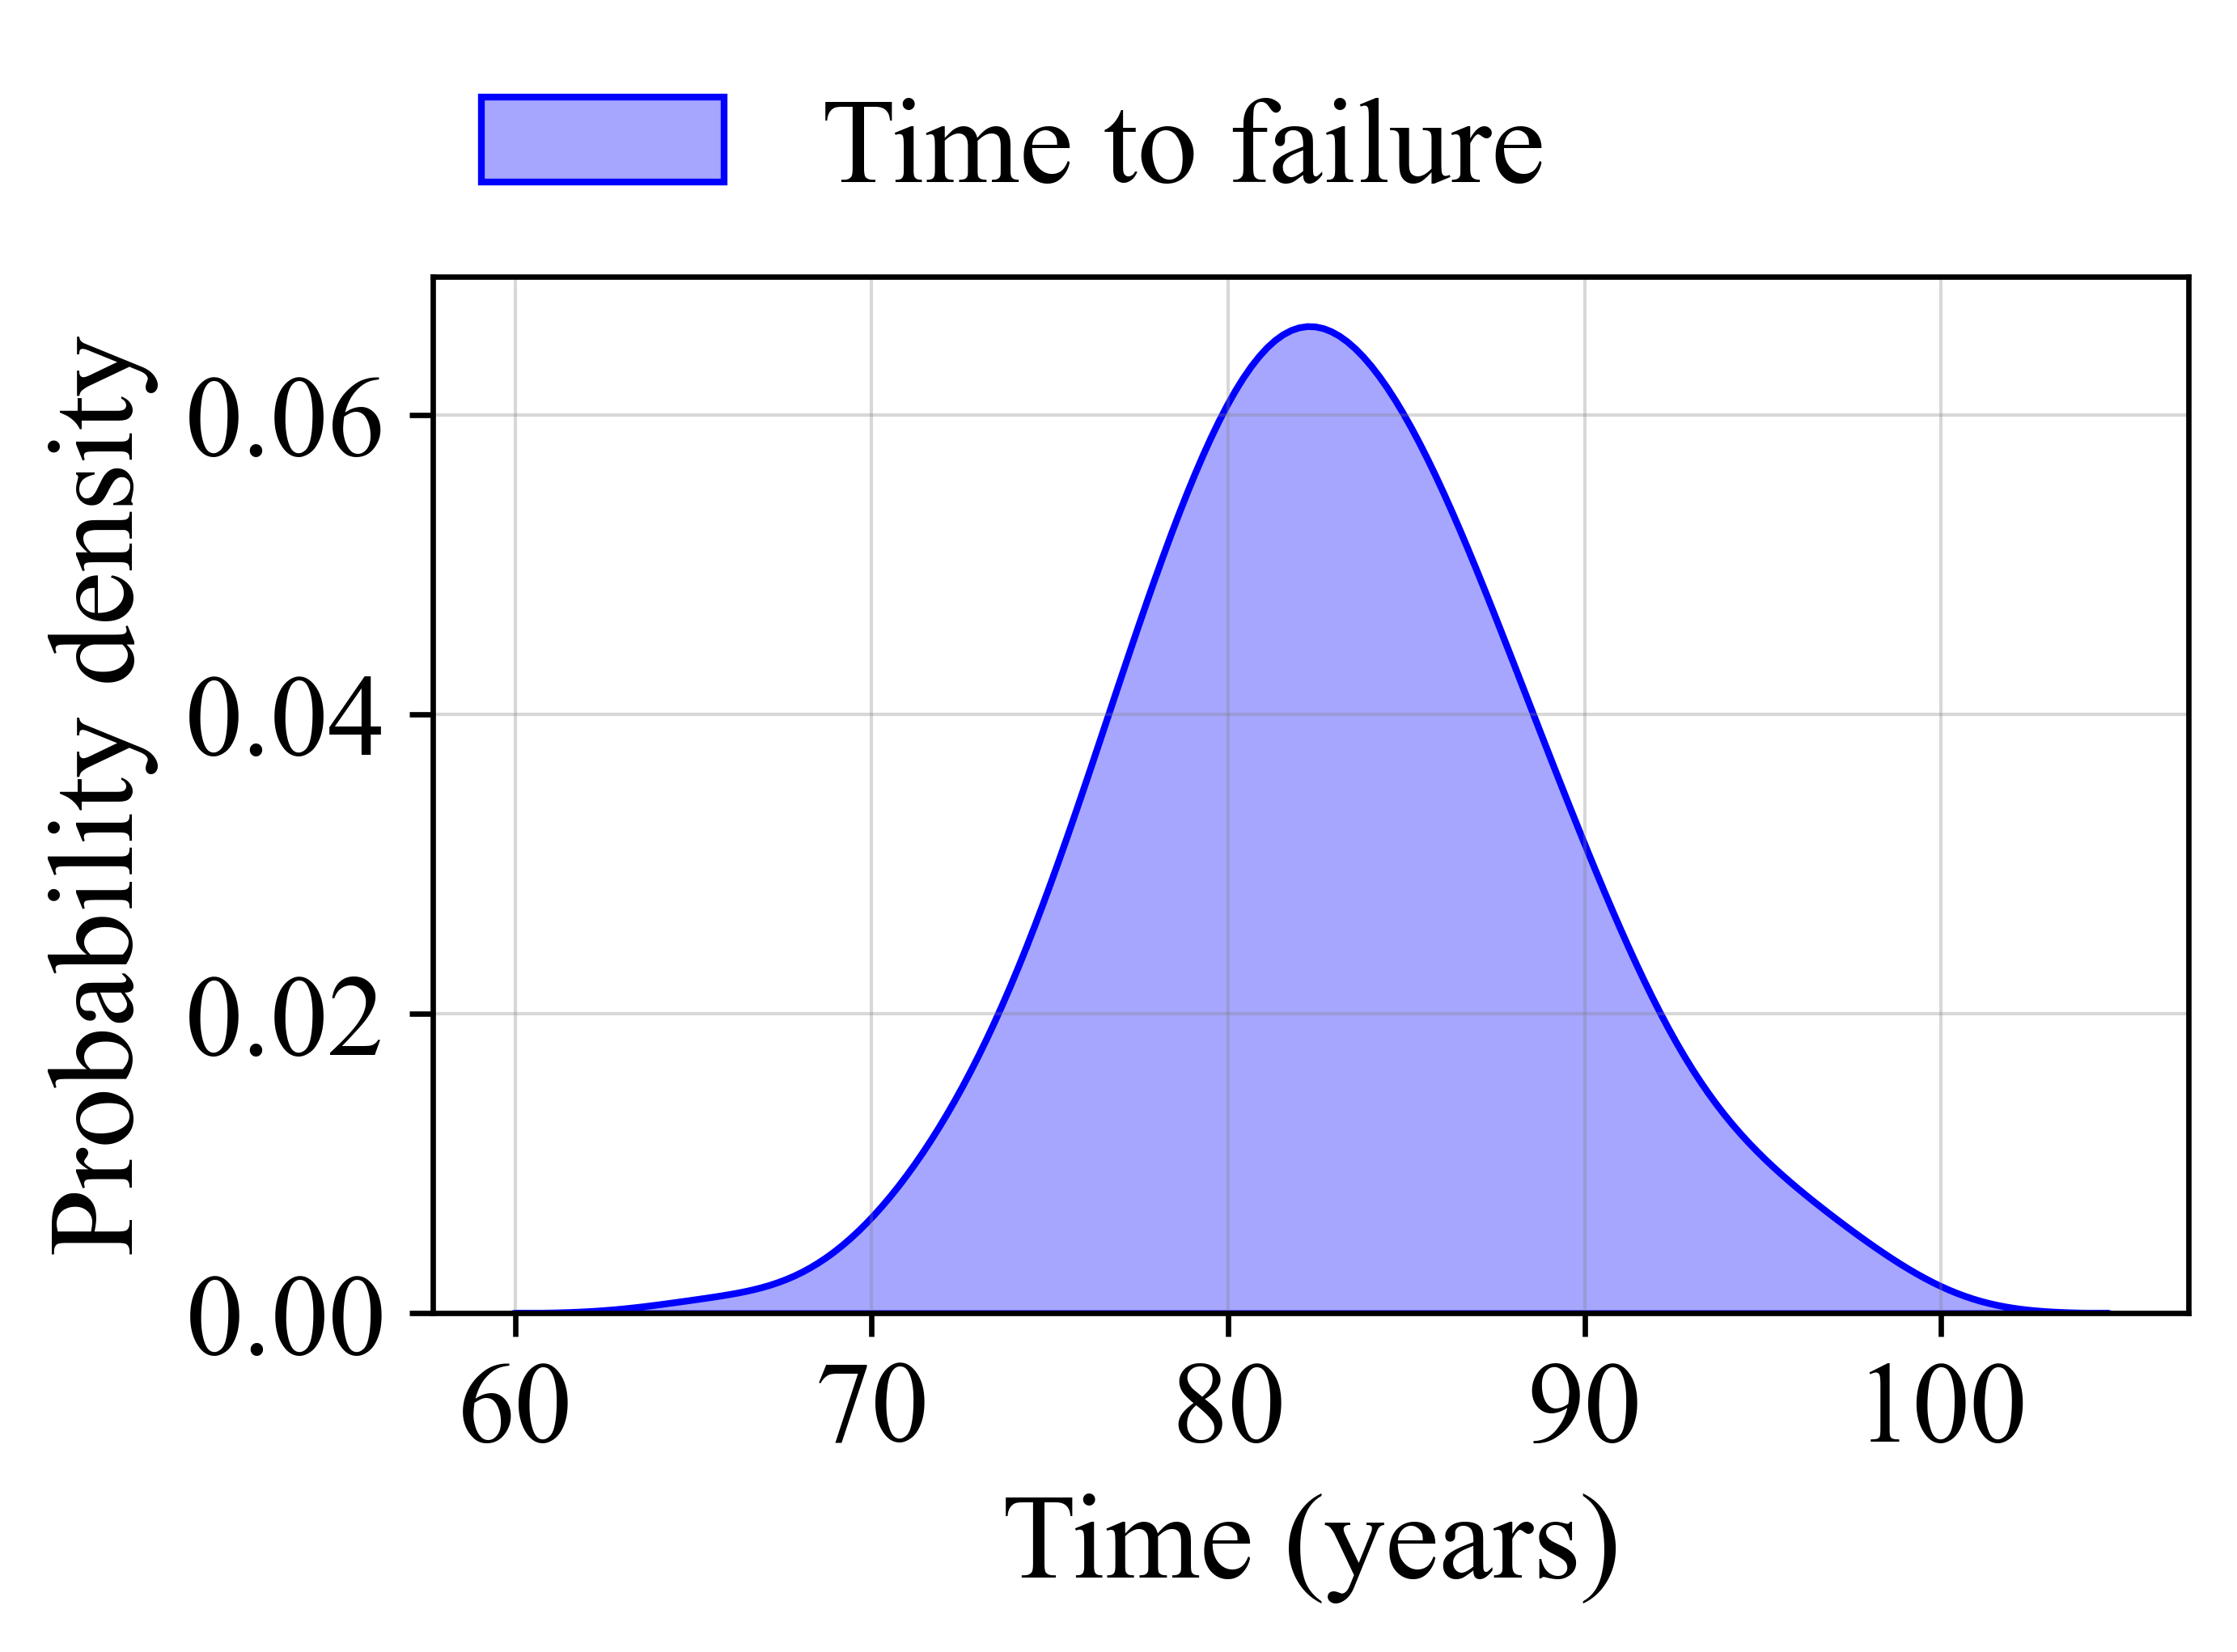
\includegraphics[
            height=4.0cm,
            keepaspectratio
        ]{z_kde_time_to_failure.png}
        \caption{Probability density of the time to failure.}
        \label{fig:kde_time_to_failure}
    \end{subfigure}
    \hfill
    \begin{subfigure}[b]{0.32\textwidth}
        \centering
        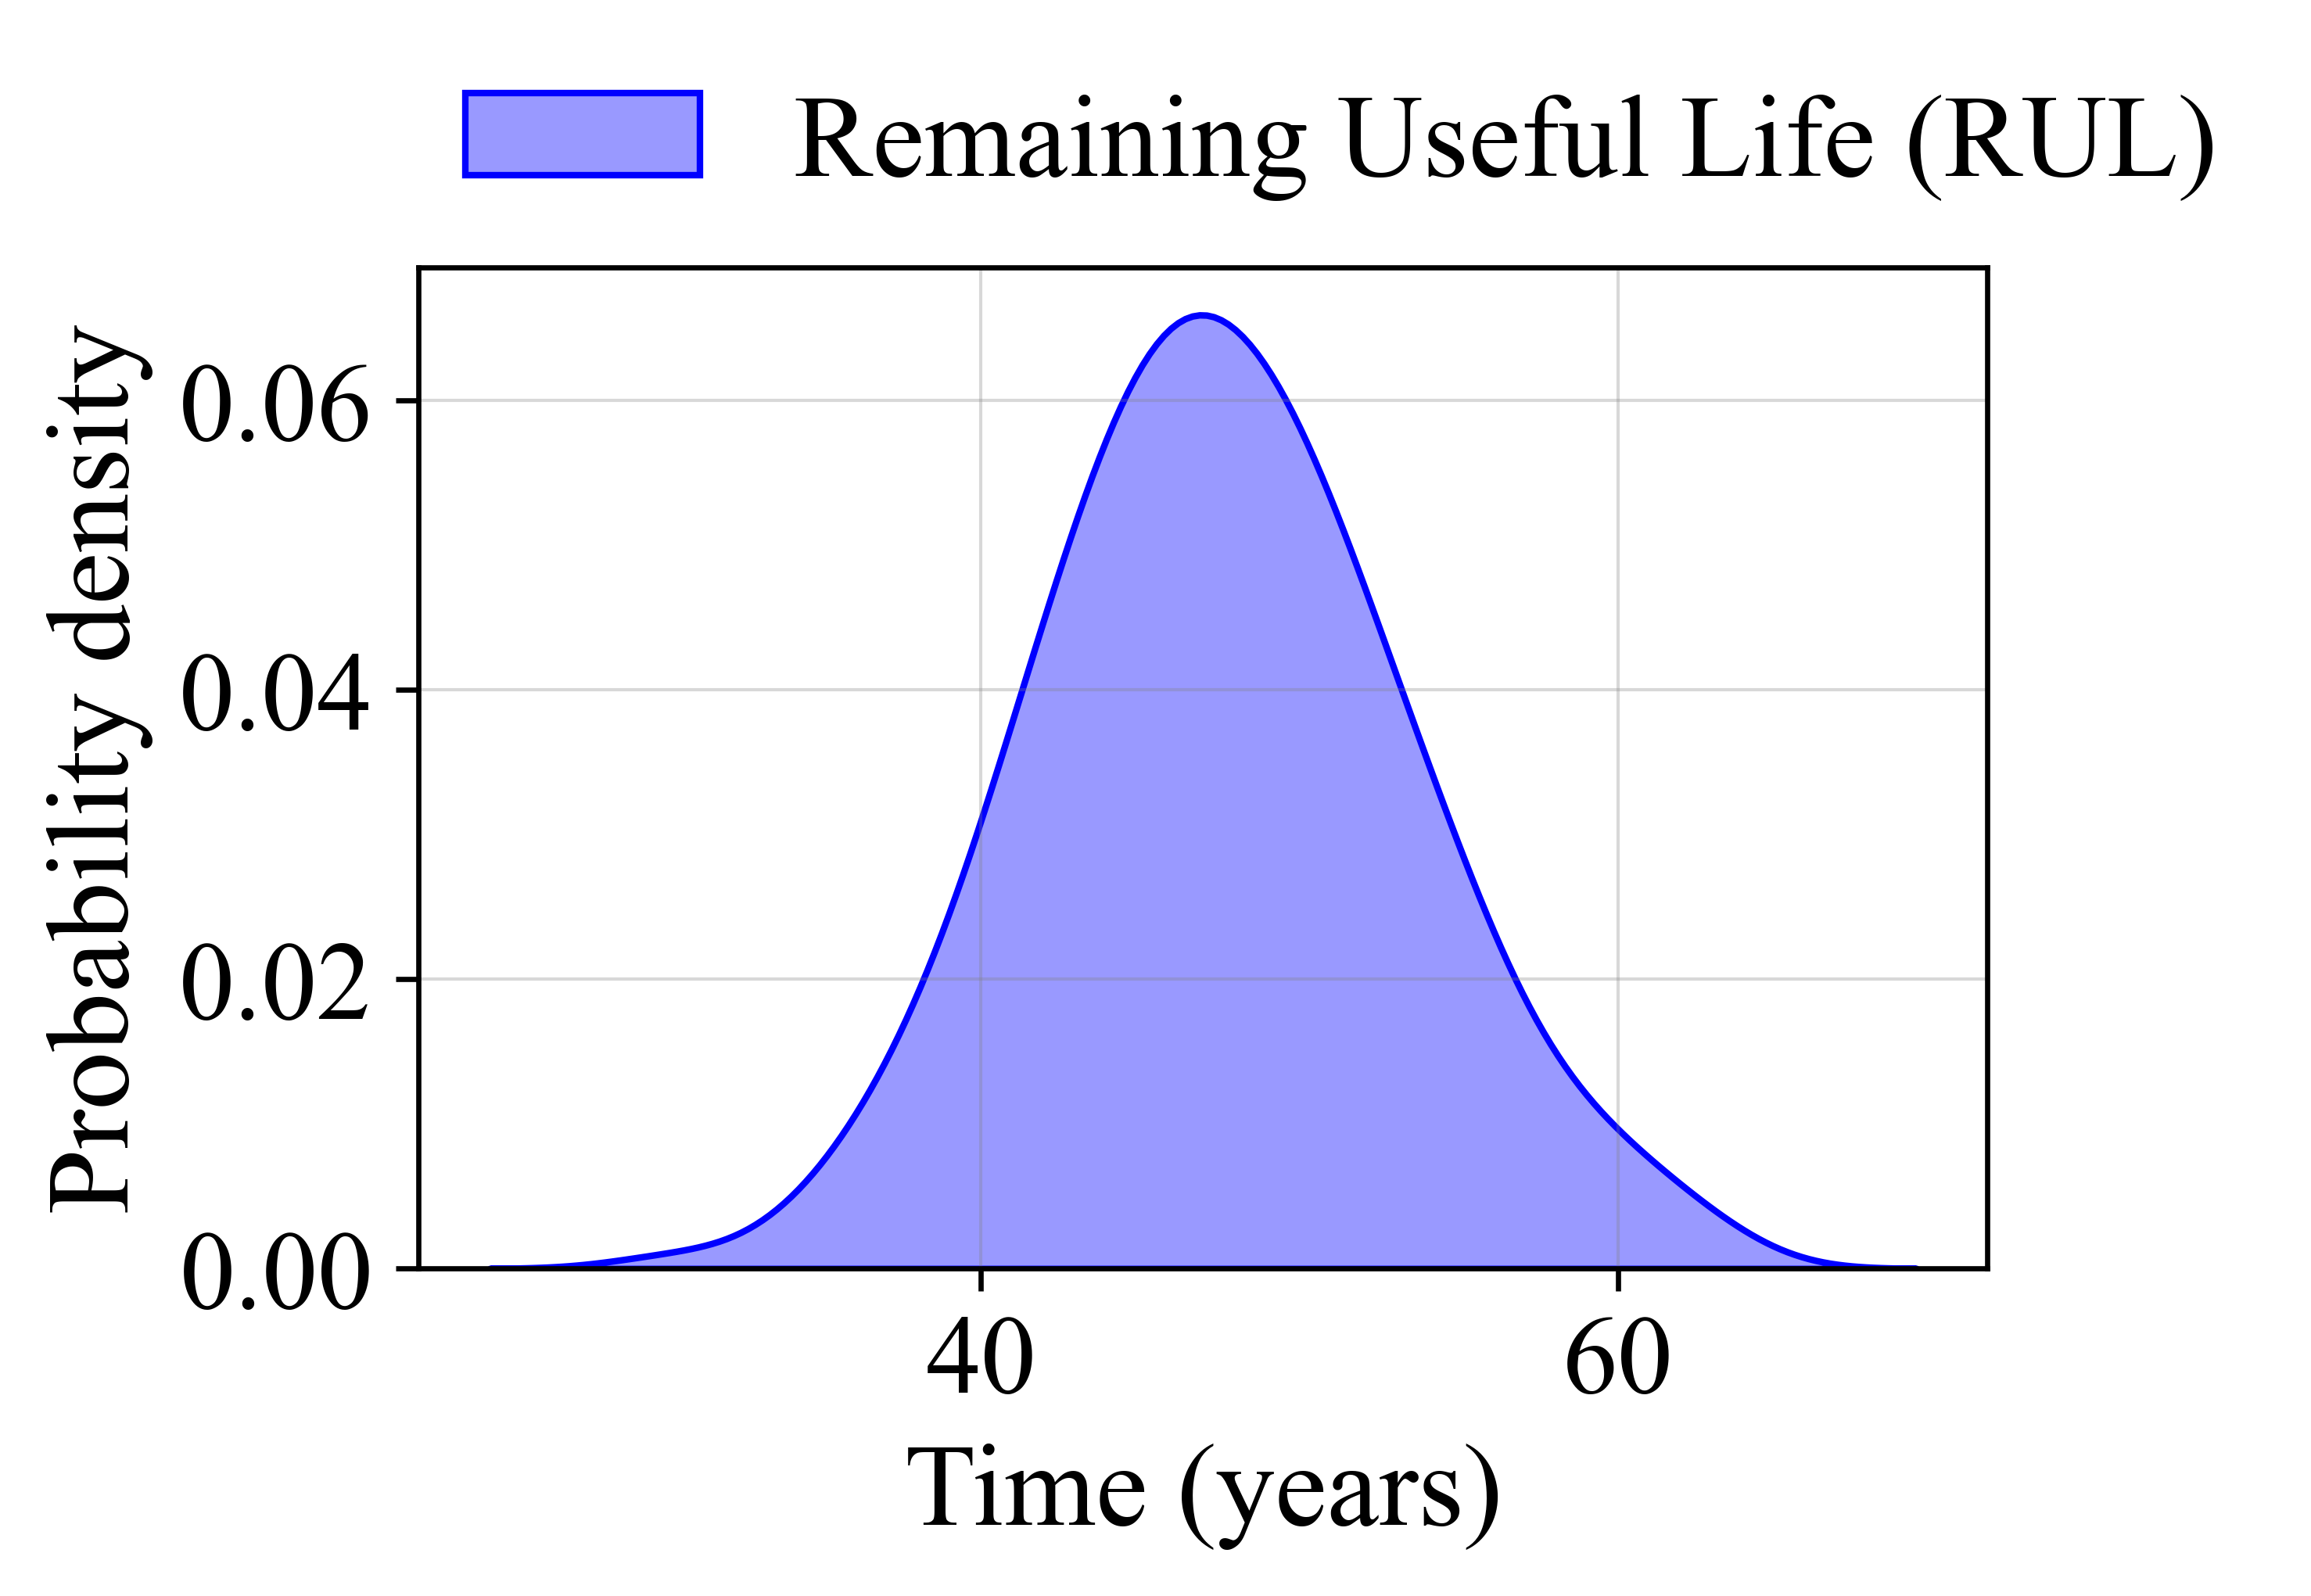
\includegraphics[
            height=4.0cm,
            keepaspectratio
        ]{z_kde_rul.png}
        \caption{KDE of the Remaining Useful Life (RUL).}
        \label{fig:kde_rul}
    \end{subfigure}

    \caption{Probabilistic results obtained from the surrogate-based framework for Remaining Useful Life (RUL) estimation: (a) distribution of the limit state function at the inspection time, (b) distribution of the time to failure, and (c) resulting RUL distribution.}
    \label{fig:rul_results}
\end{figure}

To further support decision-making under uncertainty, risk-based metrics were derived from the Remaining Useful Life (RUL) distribution, namely the Value-at-Risk (VaR) and the Conditional Value-at-Risk (CVaR). While the full probabilistic characterization of RUL provides comprehensive insight into the system behavior, these scalar metrics offer conservative indicators focused on adverse scenarios, which are particularly relevant for maintenance planning and reliability-based decision processes.

The VaR at confidence level $\alpha$ represents the lower quantile of the RUL distribution, indicating the minimum remaining life that can be expected with a confidence level of $(1-\alpha)$. In contrast, the CVaR corresponds to the expected RUL conditioned on values below the VaR threshold, explicitly accounting for tail behavior and providing a more conservative measure of risk.

In this study, both metrics were computed for $\alpha = 5\%$ using the surrogate-based RUL samples. The results are summarized in Table~\ref{tab:var_cvar_rul}. The relatively small difference between VaR and CVaR suggests limited tail severity, indicating that even under unfavorable conditions the predicted remaining life does not exhibit abrupt degradation. This behavior reinforces the robustness of the proposed surrogate framework for probabilistic RUL assessment and its suitability for reliability-informed maintenance decision-making.

\begin{table}[H]
\centering
\caption{Risk-based metrics derived from the RUL distribution for $\alpha = 5\%$.}
\label{tab:var_cvar_rul}
\begin{tabular}{lc}
\hline
\textbf{Metric} & \textbf{Value} \\
\hline
VaR$_{5\%}$ & 38.38 \\
CVaR$_{5\%}$ & 36.42 \\
\hline
\end{tabular}
\end{table}





\subsubsection{Machine Learning}

Building upon the discrete time-step analysis performed via PCE, a machine learning approach was adopted to enable the continuous prediction of the GLAM parameters $\lambda_1$ and $\lambda_2$ throughout the structural service life. While the PCE models provide accurate predictions at fixed time intervals, an Artificial Neural Network (ANN) was implemented to generalize this behavior, allowing for the estimation of the parameters at any arbitrary time $t \in [0, 100]$ years.

To train the ANN, a comprehensive synthetic dataset comprising 11,000 samples was generated using the previously validated PCE metamodels. The input space was sampled based on the probability distributions of the resistance $R$ and load $S$ defined in Table~\ref{tab:random_variables_parameters}, combined with time values uniformly distributed over the analysis horizon.

The network was trained to map the input vector $\mathbf{x} = \{R, S, t\}$ to the output vector $\mathbf{y} = \{\lambda_1, \lambda_2\}$. The dataset was randomly partitioned into training and testing subsets to evaluate the model's generalization capability and avoid overfitting.

Figure~\ref{fig:z_temporal_evolution_ann_with_points_en.pn} illustrates the temporal evolution of the GLAM parameters $\lambda_1$ and $\lambda_2$ over the 100-year service life, predicted by the trained ANN for a representative scenario ($r=5.09$, $s=1.80$). The plot demonstrates the network's ability to act as a continuous interpolator, smoothly reconstructing the degradation trajectory between the discrete time steps originally evaluated by the PCE model. The coherent behavior of the curves, free from numerical noise or discontinuities, confirms that the ANN effectively learned the underlying physics of the time-dependent degradation process.

Quantitatively, the model demonstrated excellent predictive accuracy, achieving coefficients of determination ($R^2$) of 0.9976 for $\lambda_1$ and 0.9844 for $\lambda_2$. These high correlation metrics, combined with the visual smoothness of the temporal predictions, validate the ANN as a robust and computationally efficient tool for continuous reliability assessment at any arbitrary time point within the analysis horizon.

\begin{figure}
    \centering
    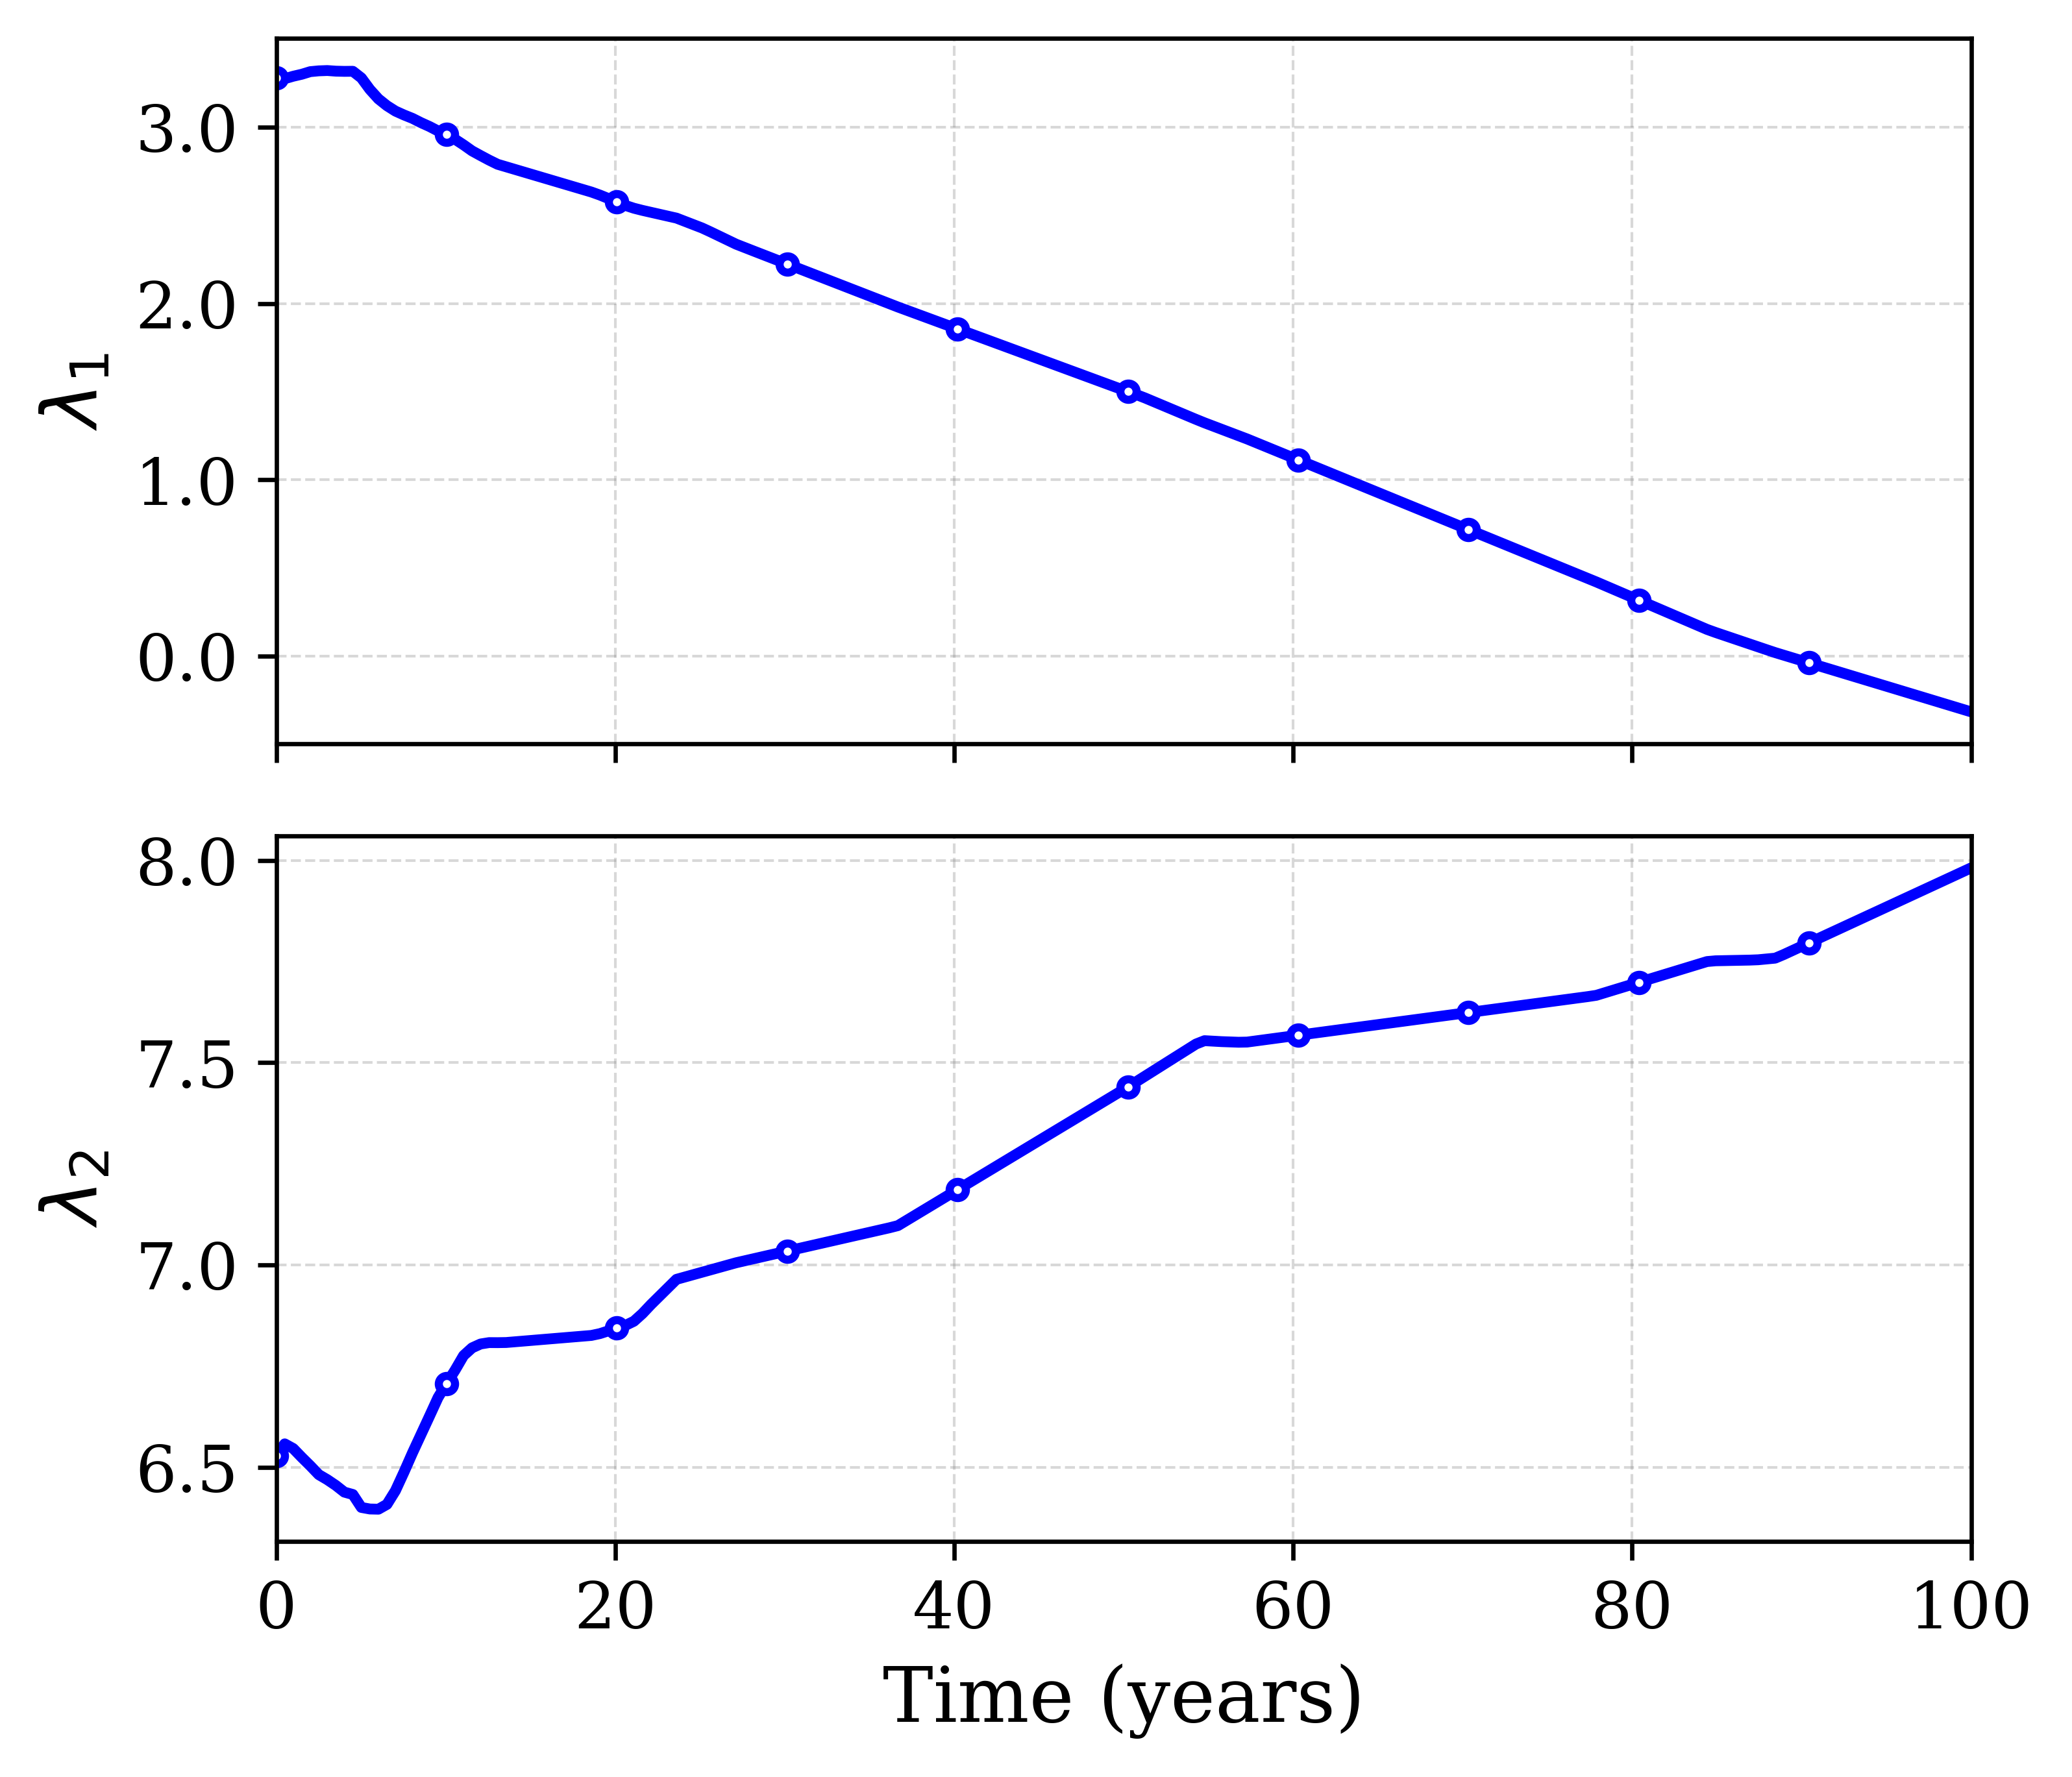
\includegraphics[width=0.75\linewidth]{z_temporal_evolution_ann_with_points_en.png}
    \caption{Temporal evolution of the GLAM parameters $\lambda_1$ and $\lambda_2$ over the service life ($t \in [0, 100]$ years) for the fixed realization $r = 5.09$ and $s = 1.80$. The continuous lines represent the ANN-based interpolation, demonstrating the model's capability to reconstruct the degradation trajectory with smoothness and consistency.}
    \label{fig:z_temporal_evolution_ann_with_points_en.pn}
\end{figure}





\section{Example}\label{sec:exem}\subsection{Modelagem Computacional da Evolução da Capacidade Resistente de Vigas de Concreto Armado sob Corrosão}

Este trabalho implementa um modelo numérico para avaliar, ao longo do tempo, a degradação da capacidade resistente à flexão de vigas de concreto armado submetidas à corrosão das armaduras. A formulação combina (i) os modelos normativos de cálculo da resistência à flexão conforme a NBR 6118:2023 e (ii) a modelagem físico-química dos efeitos da corrosão, com base em Azad e Al-Gohi (2008) e Peng e Stewart (2016). 

Apesar de o algoritmo completo realizar múltiplas simulações estocásticas em diversos passos de tempo, apresenta-se aqui apenas um passo de tempo e uma única simulação, a fim de descrever de forma clara o procedimento computacional.

\subsection{Parâmetros iniciais e propriedades mecânicas}

A viga analisada apresenta os seguintes parâmetros geométricos e mecânicos:

\begin{itemize}
    \item largura da seção: $b_w$;
    \item altura total: $h$;
    \item profundidade útil: $d = \alpha h$, com $\alpha = 0{,}90$;
    \item cobrimento nominal: $c_{\mathrm{nom}} = 25\,\text{mm}$;
    \item resistência característica do concreto: $f_{ck}$;
    \item resistência característica do aço: $f_{yk} = 500\,\text{MPa}$;
    \item módulo de elasticidade do aço: $E_s = 200\,\text{GPa}$;
    \item momento característico das ações permanentes: $M_{Gk} = 6{,}32\,\text{kN·m}$;
    \item momento característico das ações variáveis: $M_{Qk} = 1{,}381\,\text{kN·m}$.
\end{itemize}

A área inicial de armadura tracionada é

\[
A_{s,0} = 1{,}6 \times 10^{-4}\,\text{m}^2.
\]

Considerando um diâmetro nominal das barras igual a $d_b = 12{,}5\,\text{mm}$, obtém-se o número de barras:

\[
n_b = \frac{A_{s,0}}{\dfrac{\pi d_b^2}{4}}.
\]

A progressão da frente de carbonatação é modelada por:

\[
y_{\mathrm{carb}}(t) = k_c \sqrt{t}, 
\qquad
k_c = 6\,\text{mm}/\sqrt{\text{ano}}.
\]

\subsection{Modelo mecânico segundo a NBR 6118}

\subsubsection{Equilíbrio de forças na seção}

No cálculo da resistência última à flexão utiliza-se o equilíbrio entre as forças resistentes de compressão no concreto e de tração no aço:

\[
R_c(\beta) - R_s(\beta) = 0,
\]

em que $\beta = x/d$ representa a profundidade relativa da linha neutra. A força de compressão no concreto é expressa como

\[
R_c = \sigma_{cd}\, \lambda_c x b_w,
\]

onde $\sigma_{cd}$ é a tensão de cálculo do concreto comprimido. A força resistente no aço é dada por

\[
R_s = \sigma_s A_s,
\]

onde $\sigma_s$ é a tensão no aço obtida a partir do diagrama elasto-plástico definido pela norma.

A profundidade da linha neutra $x$ resulta da solução numérica da equação de equilíbrio:

\[
f(\beta) = R_c(\beta) - R_s(\beta) = 0.
\]

\subsubsection{Momento resistente sem corrosão}

Uma vez determinada a profundidade da linha neutra, o momento resistente inicial é:

\[
M_{Rd,0} = R_c \left( d - \frac{1}{2}\lambda_c x \right).
\]

\subsection{Modelagem da corrosão}

Após o início da corrosão, considerado no tempo $t_{\mathrm{ini}}$, o modelo incorpora efeitos de (i) perda de seção das barras e (ii) redução da aderência aço-concreto.

\subsubsection{Índice de corrosão ajustado pela temperatura}

Segundo Peng e Stewart (2016), o índice de corrosão ajustado à temperatura ambiente é:

\[
i_{\mathrm{corr}}(T) = i_{\mathrm{corr},20} \left[ 1 + k(T - 20) \right],
\]

com

\[
k =
\begin{cases}
0{,}073, & T > 20^\circ\text{C}, \\
0{,}025, & T < 20^\circ\text{C}, \\
0, & T = 20^\circ\text{C}.
\end{cases}
\]

\subsubsection{Perda de diâmetro da barra}

Definindo o período de corrosão como

\[
t_{\mathrm{corr}} = t - t_{\mathrm{ini}},
\]

a redução do diâmetro original $d_0$ (em mm) é dada por (Azad \& Al-Gohi, 2008):

\[
\Delta d = 0{,}0232 \, i_{\mathrm{corr}} \, t_{\mathrm{corr}}.
\]

O diâmetro residual da barra torna-se:

\[
d(t) = d_0 - \Delta d.
\]

A área efetiva da armadura é então:

\[
A_s(t) = n_b \, \frac{\pi d(t)^2}{4}.
\]

\subsubsection{Redução da aderência no aço}

O coeficiente de perda de aderência utilizado no modelo é:

\[
c_f =
\min\left[
1,\,
\dfrac{5}{\, d_0^{0{,}54} \left( i_{\mathrm{corr}}^\ast \, t_{\mathrm{corr}} \, 365 \right)^{0{,}19}}
\right],
\]

onde $i_{\mathrm{corr}}^\ast = i_{\mathrm{corr}}/1000$ é expresso em A/mm\(^2\).

\subsubsection{Momento resistente com corrosão}

A resistência à flexão degradada é calculada como:

\[
M_{Rd,\mathrm{cor}}(t) = c_f \, M_{Rd}(A_s(t)).
\]

\subsubsection{Cálculo da margem de segurança}

Uma vez obtido o momento resistente degradado $M_{Rd,\mathrm{cor}}(t)$, avalia-se o estado limite último de flexão mediante a comparação entre resistência e ações solicitantes. O momento solicitante total é definido como

\[
M_S = M_{Gk} + M_{Qk},
\]

onde $M_{Gk}$ e $M_{Qk}$ são, respectivamente, os momentos característicos das ações permanentes e variáveis.

A margem de segurança no instante $t$ é dada por

\[
G(t) = M_{Rd,\mathrm{cor}}(t) - M_S.
\]

Trata-se de uma função estado, amplamente utilizada em análises de confiabilidade estrutural. A interpretação física é direta:

\[
\begin{cases}
G(t) \ge 0, & \text{estrutura segura (estado não violado)}, \\[4pt]
G(t) < 0,  & \text{ocorrência do estado limite último}.
\end{cases}
\]

Assim, o valor de $G(t)$ indica a distância, em termos de momento fletor resistente, entre a capacidade residual da seção corroída e a demanda estrutural. A progressiva redução de $G(t)$ ao longo do tempo reflete a deterioração da barra longitudinal, tanto pela perda de seção quanto pela redução da aderência aço–concreto.

Este procedimento é repetido para todos os tempos da simulação e para todas as amostras estocásticas, permitindo a determinação de curvas de confiabilidade e da probabilidade de falha em cada ano de vida útil.

\subsection{Exemplo numérico para um único passo de tempo}

Considere o passo de tempo $t = 40$ anos, com temperatura ambiente $T = 23{,}56^\circ$C, índice de corrosão a 20°C igual a $i_{\mathrm{corr},20} = 0{,}431\,\mu\text{A/cm}^2$, diâmetro original $d_0 = 12{,}5\,\text{mm}$ e início da corrosão em $t_{\mathrm{ini}} = 25$ anos.

\subsubsection{Verificação da carbonatação}

\[
y_{\mathrm{carb}}(40) = 6\sqrt{40} = 37{,}95\,\text{mm}.
\]

Como $y_{\mathrm{carb}}(40) > c_{\mathrm{nom}} = 25\,\text{mm}$, considera-se que já ocorreu o início da corrosão.

\subsubsection{Índice de corrosão ajustado}

\[
i_{\mathrm{corr}}(23{,}56)
= 0{,}431 \, \left[ 1 + 0{,}073 (23{,}56 - 20) \right]
= 0{,}542\,\mu\text{A/cm}^2.
\]

\subsubsection{Perda de diâmetro}

\[
t_{\mathrm{corr}} = 40 - 25 = 15\,\text{anos},
\]

\[
\Delta d = 0{,}0232 \times 0{,}542 \times 15 = 0{,}1886\,\text{mm},
\]

\[
d(40) = 12{,}5 - 0{,}1886 = 12{,}3114\,\text{mm}.
\]

\subsubsection{Cálculo da área efetiva de aço}

A área da barra corroída é:

\[
A_s(40)
= \frac{\pi}{4}\,d(40)^2
= \frac{\pi}{4}(12{,}3114^2)
= 119{,}06\,\text{mm}^2.
\]

A barra original ($d_0 = 12{,}5$ mm) possuía:

\[
A_{s,0} = 122{,}72\,\text{mm}^2.
\]

Logo, há uma redução de:

\[
\Delta A_s = A_{s,0} - A_s(40) = 3{,}66\,\text{mm}^2.
\]

\subsubsection{Cálculo do momento resistente}

Com a perda de área, o momento resistente reduzido é obtido pelo equilíbrio seccional:

\[
M_{Rd}(40)
= 0{,}85\, f_{cd} \, b_w \, x \left( d - \frac{x}{2} \right),
\]

com reposicionamento neutro recalculado usando $A_s(40)$.

Considerando os parâmetros usados no código (que retornam o valor numérico):

\[
M_{Rd}(40) = 34{,}82\,\text{kN·m}.
\]

\subsubsection{Coeficiente de aderência}

O coeficiente redutor é:

\[
c_f = 
\dfrac{5}
{ d_0^{0{,}54}
\left[
(i_{\mathrm{corr}}/1000)\, t_{\mathrm{corr}}\, 365
\right]^{0{,}19}}
=
\dfrac{5}
{ 12{,}5^{0{,}54}
\left[
(0{,}542/1000)\cdot 15 \cdot 365
\right]^{0{,}19}}
= 0{,}873.
\]

Assim:

\[
M_{Rd,\mathrm{cor}}(40)
= c_f \, M_{Rd}(40)
= 0{,}873 \times 34{,}82
= 30{,}39\,\text{kN·m}.
\]

\subsection{Margem de segurança}

Os momentos solicitantes adotados no exemplo (conforme o código) são:

\[
M_{Gk} = 12{,}0\,\text{kN·m}, \qquad
M_{Qk} = 8{,}0\,\text{kN·m}.
\]

Logo:

\[
M_{Gk} + M_{Qk} = 20{,}0\,\text{kN·m}.
\]

A margem de segurança é então:

\[
G(40)
= M_{Rd,\mathrm{cor}}(40) - \bigl( M_{Gk} + M_{Qk} \bigr)
= 30{,}39 - 20{,}0
= 10{,}39\,\text{kN·m}.
\]

\[
\boxed{G(40) = 10{,}39\,\text{kN·m}}
\]

Esse resultado indica que, aos 40 anos, mesmo considerando corrosão, a seção ainda possui capacidade resistente superior às solicitações atuantes.

%%%%%%%%%%%%%%
%The high computational cost of high-fidelity codes often precludes direct Monte Carlo simulations, necessitating the use of surrogate models, also known as emulators. While Gaussian Processes~(GP) and Polynomial Chaos Expansions~(PCE) are standard for deterministic systems, they cannot be directly applied to stochastic simulators where a single evaluation is insufficient to characterize the output distribution.

Mathematically, a stochastic simulator $\mathcal{M}_S$ can be viewed as a mapping that incorporates deterministic variables and inherent randomness. For a given vector of input parameters $\mathbf{x}$ within the domain $\mathcal{D}_X$, the output is not a single deterministic value, but a random variable $Y_{\mathbf{x}}$. This relationship is formally expressed as:

\begin{equation}\mathcal{M}_S : \mathcal{D}_X \times \Omega \rightarrow \mathbb{R}, \qquad(\mathbf{x}, \omega) \mapsto \mathcal{M}_S(\mathbf{x}, \omega),\end{equation}

In this formulation, $\mathbf{x}$ represents the set of controlled input parameters (e.g., geometry, material properties), while $\omega$ denotes a random event from the probability space $\Omega$. This latent variable $\omega$ introduces the stochasticity into the system. Consequently, for a fixed input $\mathbf{x}$, the simulator produces a distribution of possible outcomes rather than a unique solution.

In the context of durability assessment of reinforced concrete, the carbonation process is influenced by several sources of uncertainty, ranging from material heterogeneity to environmental fluctuations. To effectively capture these complex probabilistic behaviors without the computational cost of exhaustive simulations, this study employs the Generalized Lambda Distribution (GLD) as a stochastic emulator. The GLD is a highly flexible four-parameter distribution family designed to approximate a wide range of parametric distributions \cite{KarianDudewicz2000, ZhuSudret2020-GLAMoriginal}.

The Generalized Lambda Distribution (GLD) is defined by its \textit{quantile function} $Q(u)$, which is the inverse of the Cumulative Distribution Function (CDF), i.e., $Q(u) = F^{-1}(u)$. This approach is particularly advantageous for stochastic emulation as it facilitates the inverse transform sampling method. In this study, we consider the Freimer-Kollia-Mudholkar-Lin (FKML) family \cite{Freimer1988}, which is defined as:

\begin{equation}
Q(u) = \lambda_1 + \frac{1}{\lambda_2} \left( \frac{u^{\lambda_3} - 1}{\lambda_3} - \frac{(1 - u)^{\lambda_4} - 1}{\lambda_4} \right)
\label{eq:GLD_quantile}
\end{equation}

where $u \in [0, 1]$ represents the cumulative probability. The distribution is governed by four parameters: $\lambda_1$ is the \textit{location} parameter, $\lambda_2$ is the \textit{scaling} parameter (with the requirement $\lambda_2 > 0$), and $\lambda_3, \lambda_4$ are the \textit{shape} parameters.

\subsection{Parameter Estimation via Method of Moments}

To calibrate the GLD emulator, the four parameters $\boldsymbol{\lambda} = \{\lambda_1, \dots, \lambda_4\}$ must be estimated from a set of model evaluations \cite{chalabi2011gld,karian2010handbook,corlu2016estimating} . In this study, we employ the \textit{Method of Moments} (MoM) \cite{lakhany2000estimating}, which consists of matching the theoretical moments of the GLD to the empirical moments computed from the sample set $\mathcal{Y} = \{y^{(1)}, \dots, y^{(N)}\}$. The first four central moments, namely the mean $\mu$, variance $\sigma^2$, skewness $\delta$, and kurtosis $\kappa$, are analytically related to the $\lambda$-parameters as follows:

\begin{align}
\mu &= \lambda_1 - \frac{1}{\lambda_2} \left( \frac{1}{\lambda_3 + 1} - \frac{1}{\lambda_4 + 1} \right) \label{eq:mean} \\
\sigma^2 &= \frac{v_2 - v_1^2}{\lambda_2^2} \label{eq:var} \\
\delta &= \frac{v_3 - 3v_1v_2 + 2v_1^3}{(v_2 - v_1^2)^{3/2}} \label{eq:skew} \\
\kappa &= \frac{v_4 - 4v_1v_3 + 6v_1^2v_2 - 3v_1^4}{(v_2 - v_1^2)^2} \label{eq:kurt}
\end{align}

In these expressions, $v_k$ denotes a non-linear function that depends solely on $\lambda_3$ and $\lambda_4$. In Eq.~\eqref{eq:vk}, $B(\cdot, \cdot)$ represents the Beta function, defined as:

\begin{equation}
v_k = \sum_{j=0}^{k} \frac{(-1)^j}{\lambda_3^{k-j} \lambda_4^j} \binom{k}{j} B(\lambda_3(k-j) + 1, \lambda_4j + 1) \label{eq:vk}
\end{equation}

The calibration of the GLD parameters is formulated as an inverse problem, where the objective is to minimize the discrepancy between the analytical moments (Eqs. \ref{eq:mean}--\ref{eq:kurt}) and the empirical moments derived from the stochastic simulator. To solve this non-linear system, the Broyden-Fletcher-Goldfarb-Shanno (BFGS) optimization algorithm was employed \cite{nocedal2006}. BFGS is a quasi-Newton method particularly suited for this type of parameter estimation due to its efficient handling of gradients and convergence properties in multi-dimensional spaces\cite{broyden1965}. The numerical procedure was implemented using PyGLAM, an in-house Python library specifically developed for the emulation of stochastic simulators using Generalized Lambda Distributions.

Using PyGLAM, Figure~\ref{fig:pyglam_fits} shows examples of fitting the GLD to traditional distributions such as the Normal, Gumbel, and Uniform.

\begin{figure}[htbp]
     \centering
     % --- Primeira Subfigura (Normal) ---
     \begin{subfigure}[b]{0.32\textwidth}
         \centering
         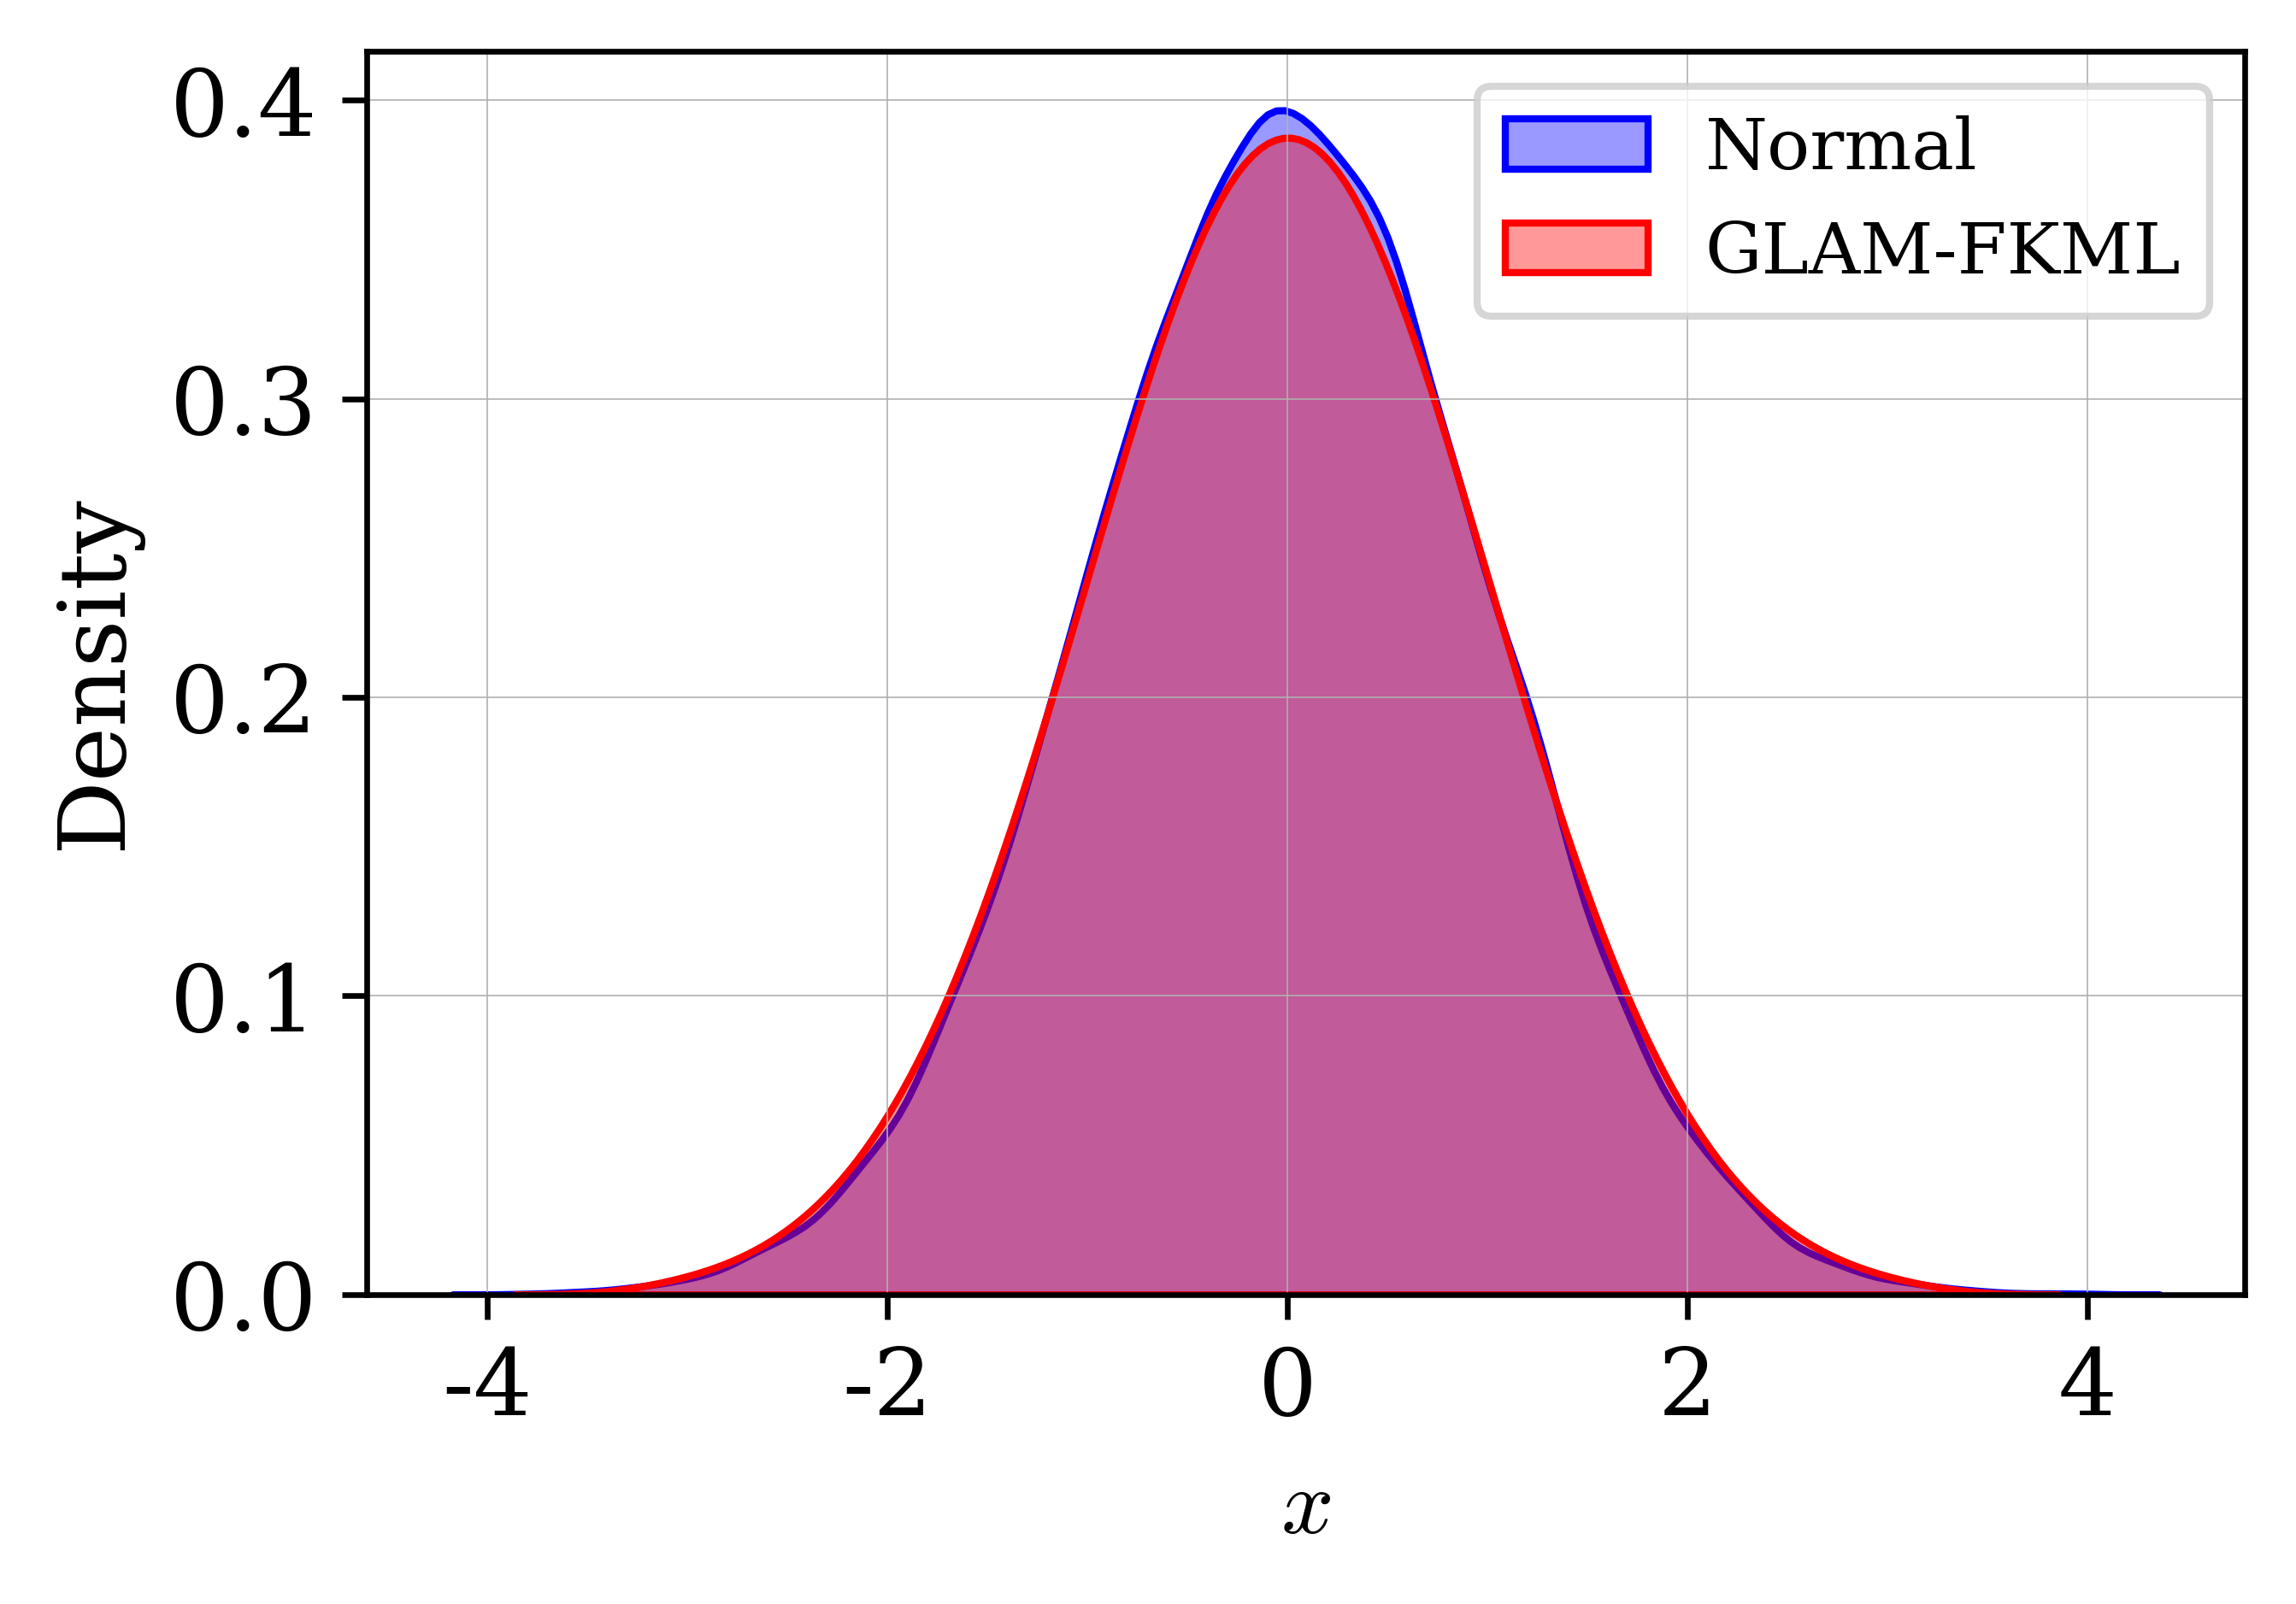
\includegraphics[width=\textwidth]{z_kde_histogram_compare.png}
         \caption{Normal distribution}
         \label{fig:fit_normal}
     \end{subfigure}
     \hfill
     % --- Segunda Subfigura (Gumbel) ---
     \begin{subfigure}[b]{0.32\textwidth}
         \centering
         \includegraphics[width=\textwidth]{fig_gumbel.pdf}
         \caption{Gumbel distribution}
         \label{fig:fit_gumbel}
     \end{subfigure}
     \hfill
     % --- Terceira Subfigura (Uniforme) ---
     \begin{subfigure}[b]{0.32\textwidth}
         \centering
         \includegraphics[width=\textwidth]{fig_uniform.pdf}
         \caption{Uniform distribution}
         \label{fig:fit_uniform}
     \end{subfigure}
     
     \caption{Validation of PyGLAM fitting capabilities for different target distributions using GLD emulators.}
     \label{fig:pyglam_fits}
\end{figure}

\subsection{Generate a emulator with Polynomial Chaos Expansion}

Following the methodology proposed by \citet{ZhuSudret2020-GLAMoriginal} and further developments in stochastic surrogate modeling, the Generalized Lambda Distribution (GLD) is coupled with Polynomial Chaos Expansion (PCE) to construct a global emulator. In this framework, the stochastic response of the simulator for any input $\mathbf{X}$ is modeled by a GLD whose parameters $\boldsymbol{\lambda}$ are themselves functions of the input variables.

Given a set of input parameters $\mathbf{X}$ governed by a joint probability density function $f_{\mathbf{X}}(\mathbf{x})$, each component of the GLD parameter vector $\lambda_i$ is approximated by a truncated PCE:

\begin{equation}
\lambda_i(\mathbf{X}) \approx \sum_{\boldsymbol{\alpha} \in \mathcal{A}} a_{i, \boldsymbol{\alpha}} \Psi_{\boldsymbol{\alpha}}(\mathbf{X}), \quad i = \{1, 2, 3, 4\}
\label{eq:pce_lambda}
\end{equation}

where $\Psi_{\boldsymbol{\alpha}}(\mathbf{X})$ are multivariate orthonormal polynomials specific to the input distributions, $a_{i, \boldsymbol{\alpha}}$ are the polynomial coefficients to be determined, and $\mathcal{A}$ is the set of multi-indices defining the truncation scheme (e.g., total degree basis).

The training procedure for the PCE-GLD emulator follows these steps:

\begin{enumerate}
    \item \textbf{Experimental Design:} A set of $M$ sample points $\{\mathbf{x}^{(1)}, \dots, \mathbf{x}^{(M)}\}$ is generated using Latin Hypercube Sampling (LHS).
    \item \textbf{Stochastic Evaluations:} For each sample point $\mathbf{x}^{(j)}$, the original stochastic simulator is executed $N$ times to obtain a local sample set of the response $\mathcal{Y}^{(j)}$.
    \item \textbf{Local GLD Fitting:} The Method of Moments, implemented via PyGLAM with the BFGS optimizer, is used to estimate the optimal local parameters $\hat{\boldsymbol{\lambda}}^{(j)}$ for each $\mathcal{Y}^{(j)}$.
    \item \textbf{PCE Coefficients Estimation:} Using the pairs $\{\mathbf{x}^{(j)}, \hat{\boldsymbol{\lambda}}^{(j)}\}_{j=1}^M$, the PCE coefficients $a_{i, \boldsymbol{\alpha}}$ are computed for each $\lambda_i$.
\end{enumerate}

Once trained, the emulator can instantly provide the complete probability distribution (via the $\lambda$ parameters) for any new input $\mathbf{X}^*$ without requiring new runs of the original stochastic simulator.

\subsection{Time-Dependent Stochastic Emulation}

The carbonation process is inherently time-dependent, requiring the evolution of the depth distribution to be captured throughout the structure's service life. To account for this, the PCE-GLD framework is extended to include time $t$ as a continuous input variable. In this temporal emulation scheme, the GLD parameters $\boldsymbol{\lambda}$ are evaluated at discrete time steps, and a machine learning (ML) surrogate is subsequently trained to map the joint input space of physical variables $\mathbf{X}$ and time $t$ to the distribution parameters.

The dataset for training the temporal emulator is constructed by evaluating the stochastic simulator at $N_t$ discrete time steps $\{t_1, t_2, \dots, t_{N_t}\}$ (e.g., 0, 10, 20, 50, and 80 years). For each time step $t_m$, a set of $M$ samples of the input vector $\mathbf{X}^{(j)}$ is evaluated, yielding the corresponding local GLD parameters $\hat{\boldsymbol{\lambda}}^{(j, m)}$ via the PyGLAM software. The resulting dataset $\mathcal{D}$ is defined as:

\begin{equation}
\mathcal{D} = \left\{ \left( \mathbf{x}^{(j)}, t_m \right), \hat{\boldsymbol{\lambda}}^{(j, m)} \right\} \quad \text{for } j=1,\dots,M \text{ and } m=1,\dots,N_t
\end{equation}

To predict the GLD parameters at any arbitrary time step $t^*$, a multi-output machine learning model is employed. The model learns the non-linear mapping $f: (\mathbf{X}, t) \to \mathbb{R}^4$:

\begin{equation}
\hat{\boldsymbol{\lambda}}(\mathbf{X}, t) \approx \mathcal{M}_{ML}(\mathbf{X}, t; \mathbf{w})
\end{equation}

where $\mathcal{M}_{ML}$ represents the chosen regressor (e.g., Random Forests, Support Vector Regression, or Neural Networks) and $\mathbf{w}$ denotes the optimized hyperparameters. By including the time step as an explicit input, the emulator can interpolate the values of $\{\lambda_1, \dots, \lambda_4\}$ between the simulated years, providing a continuous evolution of the carbonation depth PDF over the entire analysis period.

% Parametrizing the quantile function is equivalent to modeling the inverse probability integral transform. More precisely, a random variable $Y$ with $Q$ as its quantile function and a random variable $Q(U)$ with $U \sim \mathcal{U}(0,1)$ follow the same distribution. Consequently, the PDF $f_Y(y)$ of a random variable $Y$ following a GLD can be calculated through a change of variables as follows:

% \begin{equation}
% f_Y(y) = \frac{f_U(u)}{Q'(u)} = \frac{\lambda_2}{u^{\lambda_3-1} + (1 - u)^{\lambda_4-1}} \mathbb{1}_{[0,1]}(u), \quad \text{with } u = Q^{-1}(y)
% \end{equation}

% where $\mathbb{1}_{[0,1]}(u)$ is the indicator function and $Q'(u)$ denotes the derivative of the quantile function, also known as the quantile density function.




% Na prática, esta última decorre de variáveis aleatórias latentes \( \mathbf{Z}(\omega) \) (definidas sobre o mesmo espaço de probabilidade, com suporte \( \mathcal{D}_Z \subset \mathbb{R}^{M_Z} \)), que são parâmetros internos do simulador não explicitamente considerados como variáveis de entrada.  

% Em outras palavras, um simulador estocástico é construído a partir de um modelo determinístico \( \mathcal{M} \) da seguinte forma:
% \begin{equation}
% \mathcal{M}_S(\mathbf{x}, \omega) = \mathcal{M}(\mathbf{x}, \mathbf{Z}(\omega)).
% \label{eq3}
% \end{equation}

% Para um dado vetor de entrada \( \mathbf{x}_0 \), cada execução do simulador corresponde a uma realização diferente das variáveis latentes \( \mathbf{Z} \), digamos \( \mathbf{z}_0 \equiv \mathbf{Z}(\omega_0) \), e fornece uma realização particular da variável aleatória de saída \( Y_{\mathbf{x}_0} \equiv \mathcal{M}_S(\mathbf{x}_0, \cdot) \).  
% Para caracterizar a distribuição desta variável de saída, devem ser geradas repetições, isto é, múltiplas execuções de \( \mathcal{M}_S \) com o mesmo vetor de entrada \( \mathbf{x}_0 \) e diferentes realizações \(\{\mathbf{z}_1, \ldots, \mathbf{z}_R\}\) das variáveis latentes.  Referir-nos-emos à função densidade de probabilidade de \( Y_{\mathbf{x}_0} \) como a \textit{distribuição condicional da resposta} dado \( \mathbf{x}_0 \).

% Em contraste, ao fixar a realização \(z_0\) e executar o modelo para diferentes entradas, obtém-se uma
% trajetória do simulador, ou seja, uma função (padrão)  \(\mathcal{M}_S(\cdot, \omega_0) : D_X \to \mathbb{R}\). 
% Essa função pode ser obtida na prática redefinindo a semente do gerador de números aleatórios que
% gera as realizações de \(Z\) para cada \(x\). Resumos estatísticos da saída de um simulador 
% estocástico, como valor médio, variância ou quantis, também são funções padrão dos parâmetros de entrada.

 

 
\section{Time-dependent Emulator based on Generalized Lambda Distribution}The high computational cost of high-fidelity codes often precludes direct Monte Carlo simulations, necessitating the use of surrogate models, also known as emulators. While Gaussian Processes~(GP) and Polynomial Chaos Expansions~(PCE) are standard for deterministic systems, they cannot be directly applied to stochastic simulators where a single evaluation is insufficient to characterize the output distribution.

Mathematically, a stochastic simulator $\mathcal{M}_S$ can be viewed as a mapping that incorporates deterministic variables and inherent randomness. For a given vector of input parameters $\mathbf{x}$ within the domain $\mathcal{D}_X$, the output is not a single deterministic value, but a random variable $Y_{\mathbf{x}}$. This relationship is formally expressed as:

\begin{equation}\mathcal{M}_S : \mathcal{D}_X \times \Omega \rightarrow \mathbb{R}, \qquad(\mathbf{x}, \omega) \mapsto \mathcal{M}_S(\mathbf{x}, \omega),\end{equation}

In this formulation, $\mathbf{x}$ represents the set of controlled input parameters (e.g., geometry, material properties), while $\omega$ denotes a random event from the probability space $\Omega$. This latent variable $\omega$ introduces the stochasticity into the system. Consequently, for a fixed input $\mathbf{x}$, the simulator produces a distribution of possible outcomes rather than a unique solution.

In the context of durability assessment of reinforced concrete, the carbonation process is influenced by several sources of uncertainty, ranging from material heterogeneity to environmental fluctuations. To effectively capture these complex probabilistic behaviors without the computational cost of exhaustive simulations, this study employs the Generalized Lambda Distribution (GLD) as a stochastic emulator. The GLD is a highly flexible four-parameter distribution family designed to approximate a wide range of parametric distributions \cite{KarianDudewicz2000, ZhuSudret2020-GLAMoriginal}.

The Generalized Lambda Distribution (GLD) is defined by its \textit{quantile function} $Q(u)$, which is the inverse of the Cumulative Distribution Function (CDF), i.e., $Q(u) = F^{-1}(u)$. This approach is particularly advantageous for stochastic emulation as it facilitates the inverse transform sampling method. In this study, we consider the Freimer-Kollia-Mudholkar-Lin (FKML) family \cite{Freimer1988}, which is defined as:

\begin{equation}
Q(u) = \lambda_1 + \frac{1}{\lambda_2} \left( \frac{u^{\lambda_3} - 1}{\lambda_3} - \frac{(1 - u)^{\lambda_4} - 1}{\lambda_4} \right)
\label{eq:GLD_quantile}
\end{equation}

where $u \in [0, 1]$ represents the cumulative probability. The distribution is governed by four parameters: $\lambda_1$ is the \textit{location} parameter, $\lambda_2$ is the \textit{scaling} parameter (with the requirement $\lambda_2 > 0$), and $\lambda_3, \lambda_4$ are the \textit{shape} parameters.

\subsection{Parameter Estimation via Method of Moments}

To calibrate the GLD emulator, the four parameters $\boldsymbol{\lambda} = \{\lambda_1, \dots, \lambda_4\}$ must be estimated from a set of model evaluations \cite{chalabi2011gld,karian2010handbook,corlu2016estimating} . In this study, we employ the \textit{Method of Moments} (MoM) \cite{lakhany2000estimating}, which consists of matching the theoretical moments of the GLD to the empirical moments computed from the sample set $\mathcal{Y} = \{y^{(1)}, \dots, y^{(N)}\}$. The first four central moments, namely the mean $\mu$, variance $\sigma^2$, skewness $\delta$, and kurtosis $\kappa$, are analytically related to the $\lambda$-parameters as follows:

\begin{align}
\mu &= \lambda_1 - \frac{1}{\lambda_2} \left( \frac{1}{\lambda_3 + 1} - \frac{1}{\lambda_4 + 1} \right) \label{eq:mean} \\
\sigma^2 &= \frac{v_2 - v_1^2}{\lambda_2^2} \label{eq:var} \\
\delta &= \frac{v_3 - 3v_1v_2 + 2v_1^3}{(v_2 - v_1^2)^{3/2}} \label{eq:skew} \\
\kappa &= \frac{v_4 - 4v_1v_3 + 6v_1^2v_2 - 3v_1^4}{(v_2 - v_1^2)^2} \label{eq:kurt}
\end{align}

In these expressions, $v_k$ denotes a non-linear function that depends solely on $\lambda_3$ and $\lambda_4$. In Eq.~\eqref{eq:vk}, $B(\cdot, \cdot)$ represents the Beta function, defined as:

\begin{equation}
v_k = \sum_{j=0}^{k} \frac{(-1)^j}{\lambda_3^{k-j} \lambda_4^j} \binom{k}{j} B(\lambda_3(k-j) + 1, \lambda_4j + 1) \label{eq:vk}
\end{equation}

The calibration of the GLD parameters is formulated as an inverse problem, where the objective is to minimize the discrepancy between the analytical moments (Eqs. \ref{eq:mean}--\ref{eq:kurt}) and the empirical moments derived from the stochastic simulator. To solve this non-linear system, the Broyden-Fletcher-Goldfarb-Shanno (BFGS) optimization algorithm was employed \cite{nocedal2006}. BFGS is a quasi-Newton method particularly suited for this type of parameter estimation due to its efficient handling of gradients and convergence properties in multi-dimensional spaces\cite{broyden1965}. The numerical procedure was implemented using PyGLAM, an in-house Python library specifically developed for the emulation of stochastic simulators using Generalized Lambda Distributions.

Using PyGLAM, Figure~\ref{fig:pyglam_fits} shows examples of fitting the GLD to traditional distributions such as the Normal, Gumbel, and Uniform.

\begin{figure}[htbp]
     \centering
     % --- Primeira Subfigura (Normal) ---
     \begin{subfigure}[b]{0.32\textwidth}
         \centering
         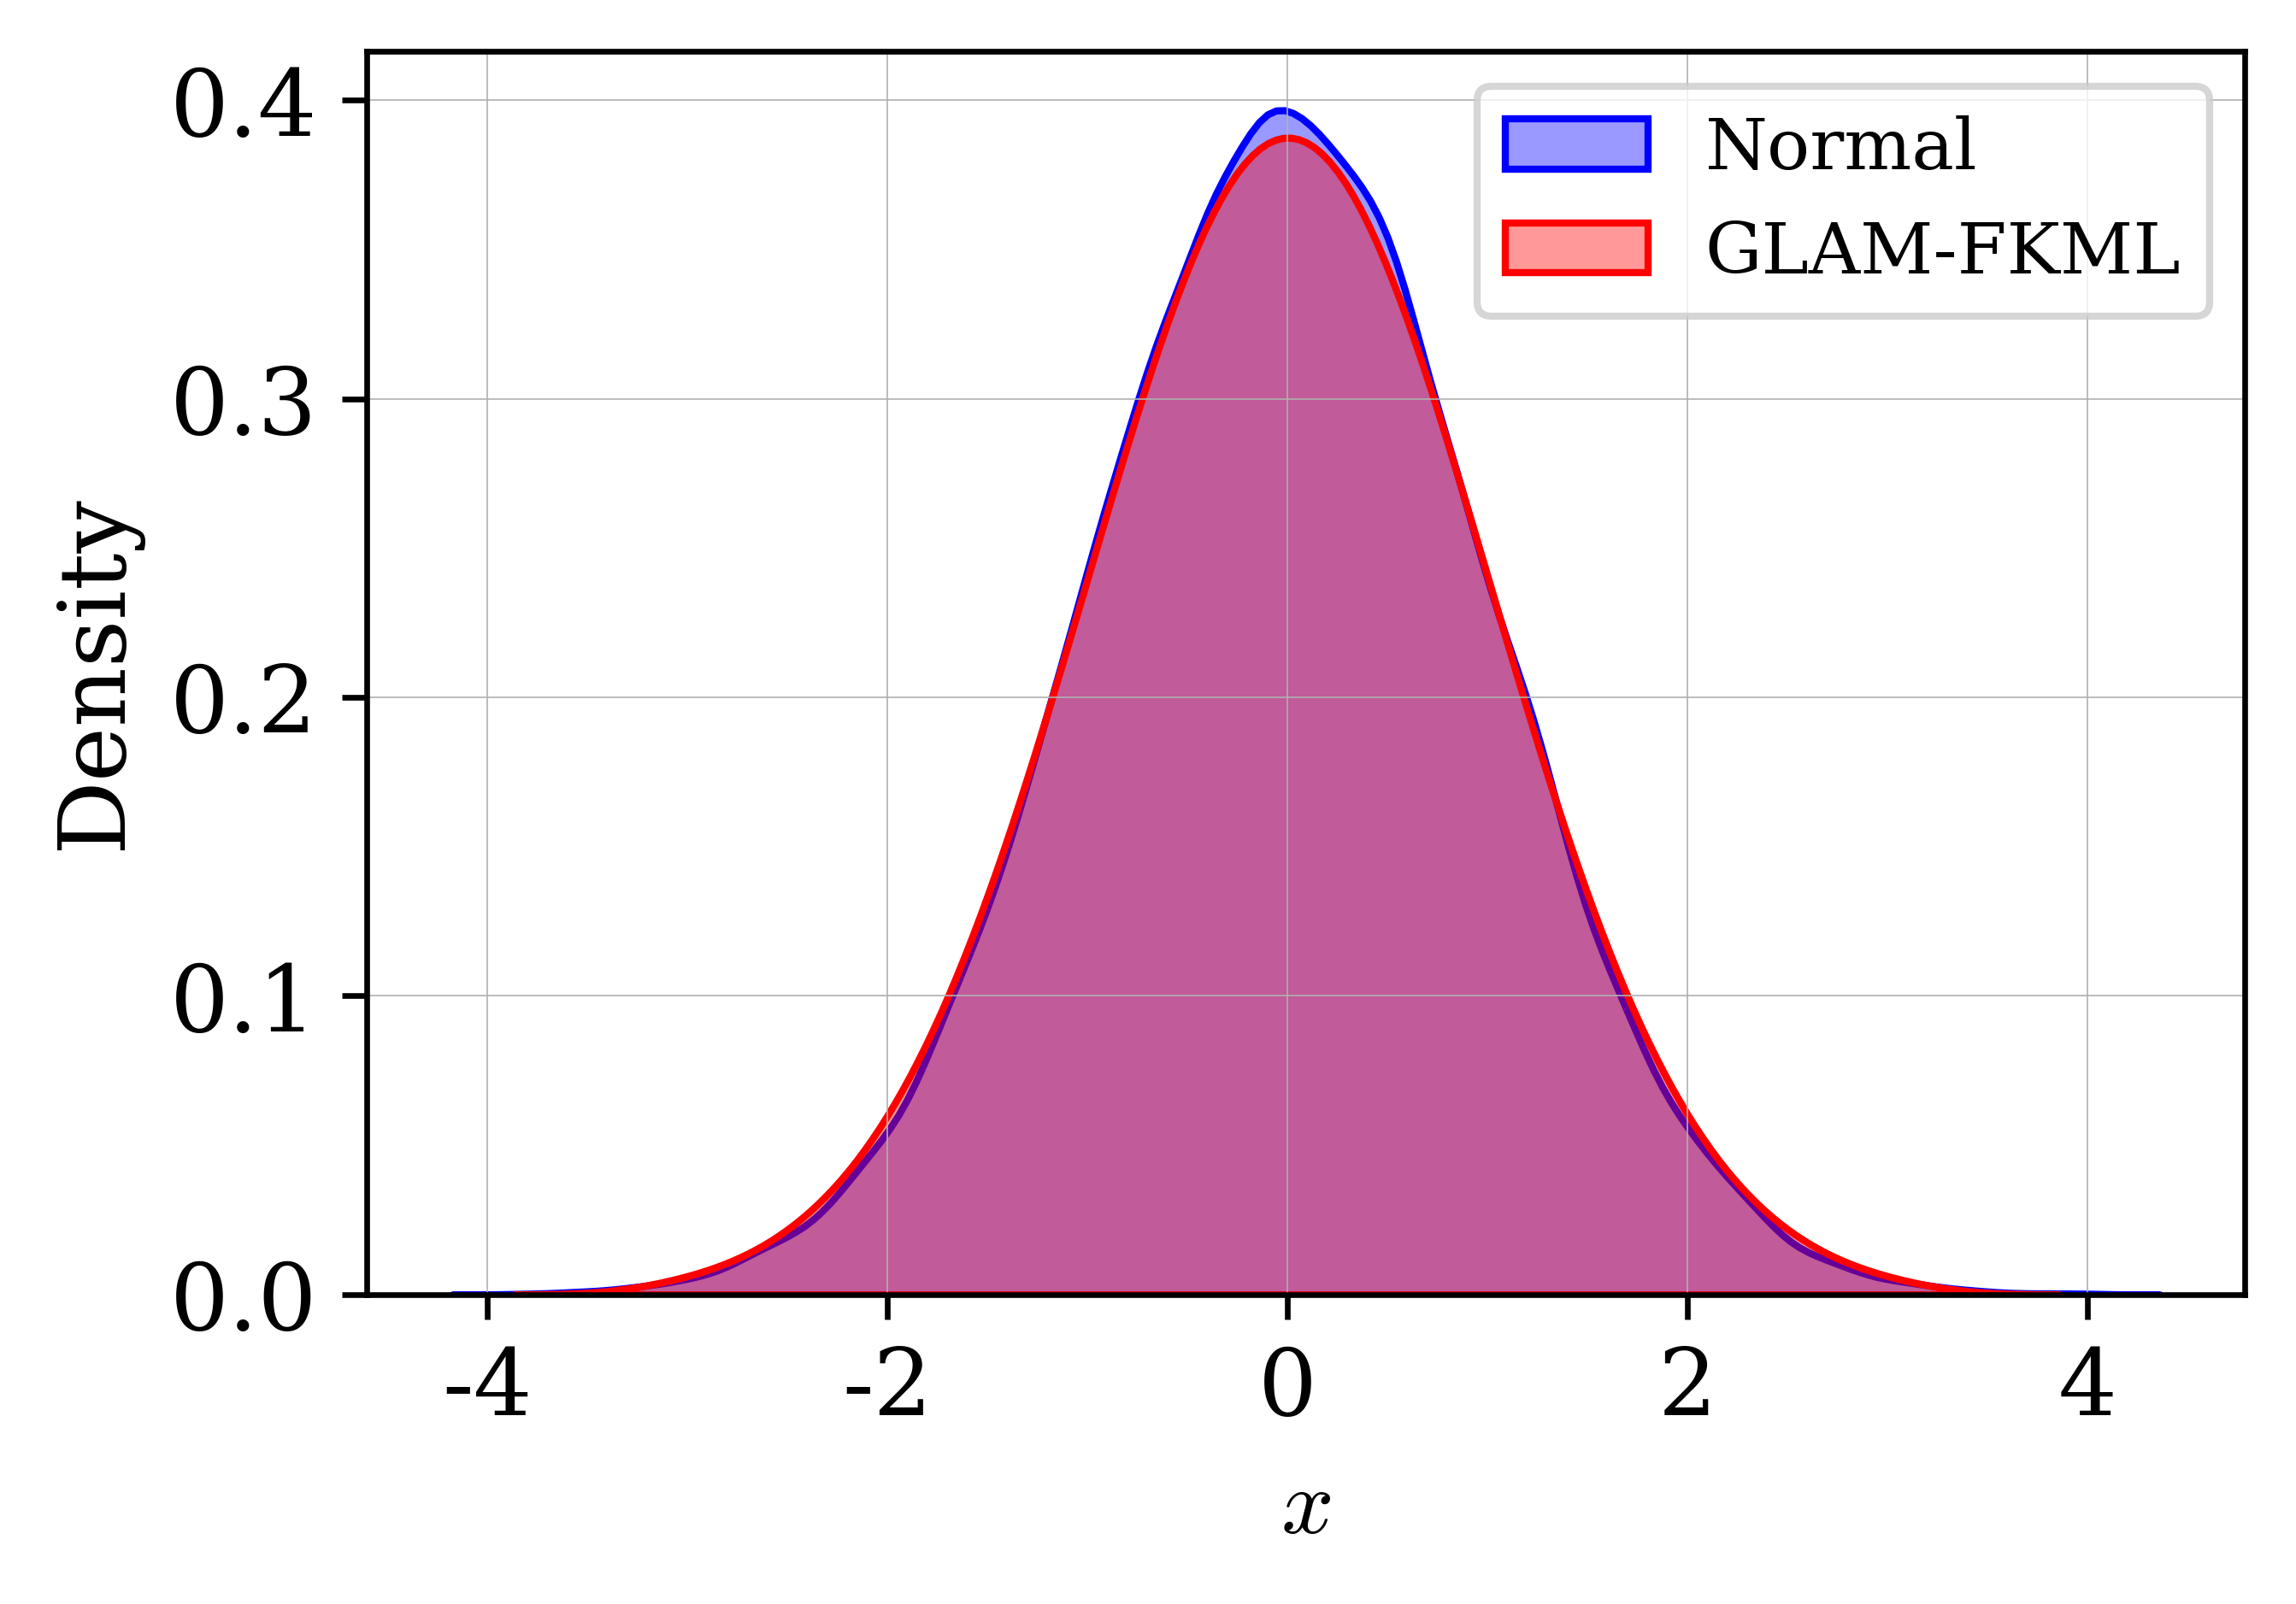
\includegraphics[width=\textwidth]{z_kde_histogram_compare.png}
         \caption{Normal distribution}
         \label{fig:fit_normal}
     \end{subfigure}
     \hfill
     % --- Segunda Subfigura (Gumbel) ---
     \begin{subfigure}[b]{0.32\textwidth}
         \centering
         \includegraphics[width=\textwidth]{fig_gumbel.pdf}
         \caption{Gumbel distribution}
         \label{fig:fit_gumbel}
     \end{subfigure}
     \hfill
     % --- Terceira Subfigura (Uniforme) ---
     \begin{subfigure}[b]{0.32\textwidth}
         \centering
         \includegraphics[width=\textwidth]{fig_uniform.pdf}
         \caption{Uniform distribution}
         \label{fig:fit_uniform}
     \end{subfigure}
     
     \caption{Validation of PyGLAM fitting capabilities for different target distributions using GLD emulators.}
     \label{fig:pyglam_fits}
\end{figure}

\subsection{Generate a emulator with Polynomial Chaos Expansion}

Following the methodology proposed by \citet{ZhuSudret2020-GLAMoriginal} and further developments in stochastic surrogate modeling, the Generalized Lambda Distribution (GLD) is coupled with Polynomial Chaos Expansion (PCE) to construct a global emulator. In this framework, the stochastic response of the simulator for any input $\mathbf{X}$ is modeled by a GLD whose parameters $\boldsymbol{\lambda}$ are themselves functions of the input variables.

Given a set of input parameters $\mathbf{X}$ governed by a joint probability density function $f_{\mathbf{X}}(\mathbf{x})$, each component of the GLD parameter vector $\lambda_i$ is approximated by a truncated PCE:

\begin{equation}
\lambda_i(\mathbf{X}) \approx \sum_{\boldsymbol{\alpha} \in \mathcal{A}} a_{i, \boldsymbol{\alpha}} \Psi_{\boldsymbol{\alpha}}(\mathbf{X}), \quad i = \{1, 2, 3, 4\}
\label{eq:pce_lambda}
\end{equation}

where $\Psi_{\boldsymbol{\alpha}}(\mathbf{X})$ are multivariate orthonormal polynomials specific to the input distributions, $a_{i, \boldsymbol{\alpha}}$ are the polynomial coefficients to be determined, and $\mathcal{A}$ is the set of multi-indices defining the truncation scheme (e.g., total degree basis).

The training procedure for the PCE-GLD emulator follows these steps:

\begin{enumerate}
    \item \textbf{Experimental Design:} A set of $M$ sample points $\{\mathbf{x}^{(1)}, \dots, \mathbf{x}^{(M)}\}$ is generated using Latin Hypercube Sampling (LHS).
    \item \textbf{Stochastic Evaluations:} For each sample point $\mathbf{x}^{(j)}$, the original stochastic simulator is executed $N$ times to obtain a local sample set of the response $\mathcal{Y}^{(j)}$.
    \item \textbf{Local GLD Fitting:} The Method of Moments, implemented via PyGLAM with the BFGS optimizer, is used to estimate the optimal local parameters $\hat{\boldsymbol{\lambda}}^{(j)}$ for each $\mathcal{Y}^{(j)}$.
    \item \textbf{PCE Coefficients Estimation:} Using the pairs $\{\mathbf{x}^{(j)}, \hat{\boldsymbol{\lambda}}^{(j)}\}_{j=1}^M$, the PCE coefficients $a_{i, \boldsymbol{\alpha}}$ are computed for each $\lambda_i$.
\end{enumerate}

Once trained, the emulator can instantly provide the complete probability distribution (via the $\lambda$ parameters) for any new input $\mathbf{X}^*$ without requiring new runs of the original stochastic simulator.

\subsection{Time-Dependent Stochastic Emulation}

The carbonation process is inherently time-dependent, requiring the evolution of the depth distribution to be captured throughout the structure's service life. To account for this, the PCE-GLD framework is extended to include time $t$ as a continuous input variable. In this temporal emulation scheme, the GLD parameters $\boldsymbol{\lambda}$ are evaluated at discrete time steps, and a machine learning (ML) surrogate is subsequently trained to map the joint input space of physical variables $\mathbf{X}$ and time $t$ to the distribution parameters.

The dataset for training the temporal emulator is constructed by evaluating the stochastic simulator at $N_t$ discrete time steps $\{t_1, t_2, \dots, t_{N_t}\}$ (e.g., 0, 10, 20, 50, and 80 years). For each time step $t_m$, a set of $M$ samples of the input vector $\mathbf{X}^{(j)}$ is evaluated, yielding the corresponding local GLD parameters $\hat{\boldsymbol{\lambda}}^{(j, m)}$ via the PyGLAM software. The resulting dataset $\mathcal{D}$ is defined as:

\begin{equation}
\mathcal{D} = \left\{ \left( \mathbf{x}^{(j)}, t_m \right), \hat{\boldsymbol{\lambda}}^{(j, m)} \right\} \quad \text{for } j=1,\dots,M \text{ and } m=1,\dots,N_t
\end{equation}

To predict the GLD parameters at any arbitrary time step $t^*$, a multi-output machine learning model is employed. The model learns the non-linear mapping $f: (\mathbf{X}, t) \to \mathbb{R}^4$:

\begin{equation}
\hat{\boldsymbol{\lambda}}(\mathbf{X}, t) \approx \mathcal{M}_{ML}(\mathbf{X}, t; \mathbf{w})
\end{equation}

where $\mathcal{M}_{ML}$ represents the chosen regressor (e.g., Random Forests, Support Vector Regression, or Neural Networks) and $\mathbf{w}$ denotes the optimized hyperparameters. By including the time step as an explicit input, the emulator can interpolate the values of $\{\lambda_1, \dots, \lambda_4\}$ between the simulated years, providing a continuous evolution of the carbonation depth PDF over the entire analysis period.

% Parametrizing the quantile function is equivalent to modeling the inverse probability integral transform. More precisely, a random variable $Y$ with $Q$ as its quantile function and a random variable $Q(U)$ with $U \sim \mathcal{U}(0,1)$ follow the same distribution. Consequently, the PDF $f_Y(y)$ of a random variable $Y$ following a GLD can be calculated through a change of variables as follows:

% \begin{equation}
% f_Y(y) = \frac{f_U(u)}{Q'(u)} = \frac{\lambda_2}{u^{\lambda_3-1} + (1 - u)^{\lambda_4-1}} \mathbb{1}_{[0,1]}(u), \quad \text{with } u = Q^{-1}(y)
% \end{equation}

% where $\mathbb{1}_{[0,1]}(u)$ is the indicator function and $Q'(u)$ denotes the derivative of the quantile function, also known as the quantile density function.




% Na prática, esta última decorre de variáveis aleatórias latentes \( \mathbf{Z}(\omega) \) (definidas sobre o mesmo espaço de probabilidade, com suporte \( \mathcal{D}_Z \subset \mathbb{R}^{M_Z} \)), que são parâmetros internos do simulador não explicitamente considerados como variáveis de entrada.  

% Em outras palavras, um simulador estocástico é construído a partir de um modelo determinístico \( \mathcal{M} \) da seguinte forma:
% \begin{equation}
% \mathcal{M}_S(\mathbf{x}, \omega) = \mathcal{M}(\mathbf{x}, \mathbf{Z}(\omega)).
% \label{eq3}
% \end{equation}

% Para um dado vetor de entrada \( \mathbf{x}_0 \), cada execução do simulador corresponde a uma realização diferente das variáveis latentes \( \mathbf{Z} \), digamos \( \mathbf{z}_0 \equiv \mathbf{Z}(\omega_0) \), e fornece uma realização particular da variável aleatória de saída \( Y_{\mathbf{x}_0} \equiv \mathcal{M}_S(\mathbf{x}_0, \cdot) \).  
% Para caracterizar a distribuição desta variável de saída, devem ser geradas repetições, isto é, múltiplas execuções de \( \mathcal{M}_S \) com o mesmo vetor de entrada \( \mathbf{x}_0 \) e diferentes realizações \(\{\mathbf{z}_1, \ldots, \mathbf{z}_R\}\) das variáveis latentes.  Referir-nos-emos à função densidade de probabilidade de \( Y_{\mathbf{x}_0} \) como a \textit{distribuição condicional da resposta} dado \( \mathbf{x}_0 \).

% Em contraste, ao fixar a realização \(z_0\) e executar o modelo para diferentes entradas, obtém-se uma
% trajetória do simulador, ou seja, uma função (padrão)  \(\mathcal{M}_S(\cdot, \omega_0) : D_X \to \mathbb{R}\). 
% Essa função pode ser obtida na prática redefinindo a semente do gerador de números aleatórios que
% gera as realizações de \(Z\) para cada \(x\). Resumos estatísticos da saída de um simulador 
% estocástico, como valor médio, variância ou quantis, também são funções padrão dos parâmetros de entrada.

 

 
%%%%%%%%%%%%%
\bibliographystyle{model1-num-names}
\bibliography{mybibfile.bib}

\end{document}
